%%%%%%%%%%%%%%%%%%%%%%%%%%%%%%%%%%%%%%%%
% datoteka diploma-vzorec.tex
%
% vzorčna datoteka za pisanje diplomskega dela v formatu LaTeX
% na UL Fakulteti za računalništvo in informatiko
%
% vkup spravil Gašper Fijavž, december 2010
% množica popravkov v januarju, februarju marcu 2011
% verzija 29. marec 2011

\documentclass[a4paper, 12pt]{book}

\usepackage[utf8x]{inputenc}   % omogoča uporabo slovenskih črk kodiranih v formatu UTF-8 
\usepackage[slovene,english]{babel}    % naloži, med drugim, slovenske delilne vzorce
\usepackage[pdftex]{graphicx}  % omogoča vlaganje slik različnih formatov 
\usepackage{fancyhdr}          % poskrbi, na primer, za glave strani

\usepackage{graphicx}
\usepackage{wrapfig}
\usepackage{latexsym}
\usepackage{amssymb}           % dodatni simboli
\usepackage{amsmath}           % eqref, npr.
\usepackage{amsthm}
\usepackage{ifthen}
\usepackage{clrscode3e}
\usepackage{fancybox}
\usepackage{filecontents}
\usepackage{varwidth}
\usepackage{afterpage}
\usepackage{placeins}

\usepackage{float}
\usepackage{algorithm}
\usepackage[noend]{algpseudocode}
\usepackage{listings}
\usepackage{framed}

\usepackage{caption}
\captionsetup[lstlisting]{font={small,tt}}
\usepackage{color}
\usepackage{textcomp}


\usepackage[mathlines]{lineno}
\usepackage{titlesec}



%\newtheorem{theorem}{Theorem}
%\newtheorem{corollary}[theorem]{Corollary}
%\newtheorem{lemma}[theorem]{Lemma}
%\newtheorem{problem}[theorem]{Problem}
%\newtheorem{proposition}[theorem]{Proposition}
%\newtheorem{conjecture}[theorem]{Conjecture}

\renewcommand{\baselinestretch}{1.3} % ustrezen razmik med vrsticami

%oznake strani
\renewcommand{\chaptermark}[1]%
{\markboth{\MakeUppercase{\thechapter.\ #1}}{}} \renewcommand{\sectionmark}[1]%
{\markright{\MakeUppercase{\thesection.\ #1}}} \renewcommand{\headrulewidth}{0.5pt} \renewcommand{\footrulewidth}{0pt} 
\fancyhf{}
\fancyhead[LE,RO]{\sl \thepage} \fancyhead[LO]{\sl \rightmark} \fancyhead[RE]{\sl \leftmark}

\newcommand{\BibTeX}{{\sc Bib}\TeX}

\newcommand{\autfont}{\Large}
\newcommand{\titfont}{\LARGE\bf}
\newcommand{\D}{\ensuremath{\mathcal{D}}} 
\newcommand{\LL}{\ensuremath{\mathbb L}}
\newcommand{\RR}{\ensuremath{\mathbb R}}  % real numbers 
\newcommand{\NN}{\ensuremath{\mathbb N}}  % natural numbers 
\newcommand{\GG}{\ensuremath{G_{\le 1}}}
\newcommand{\T}{\ensuremath{\mathcal{T}}} 
\newcommand{\OO}{\ensuremath{\mathcal{O}}} % big O notation
\newcommand{\U}{\texttt{\_}}
\newcommand{\clearemptydoublepage}{\newpage{\pagestyle{empty}\cleardoublepage}}
\setcounter{tocdepth}{1}	      % globina kazala
\setcounter{secnumdepth}{4}
\def\length{\mathrm{len}}

% konstrukti
\newtheorem{izrek}{Izrek}[chapter]
%\newtheorem{trditev}{Trditev}[izrek]
\newtheorem{lema}[izrek]{Lema}
\newenvironment{dokaz}{\emph{Dokaz.}\ }{\hspace{\fill}{$\Box$}}

\def\best{\mathit{best}}
\def\dist{\mathit{dist}}
\newcommand{\cycle}{\mathit{cycle}}
\newcommand{\walk}{\mathit{walk}}
\newcommand\CR{\mbox{\tt cr}_2}		  % crossing number

\definecolor{listinggray}{gray}{0.9}
\definecolor{lbcolor}{rgb}{0.9,0.9,0.9}
\definecolor{darkgreen}{rgb}{0.0, 0.2, 0.13}
%\lstdefinestyle{customc}{
%  belowcaptionskip=1\baselineskip,
%  breaklines=true,
%  frame=L,
%  xleftmargin=\parindent,
%  language=C,
%  showstringspaces=false,
%  basicstyle=\footnotesize\ttfamily,
%  keywordstyle=\bfseries\color{red},
%  commentstyle=\itshape\color{green},
%  identifierstyle=\color{blue},
%  stringstyle=\color{orange},
%}

%\lstset{escapechar=@,style=customc}
%\lstset{
%%backgroundcolor=\color{lbcolor},
%    tabsize=4,    
%%   rulecolor=,
%    language=C++,
%        basicstyle=\scriptsize,
%        upquote=true,
%        aboveskip={1.5\baselineskip},
%        columns=fixed,
%        showstringspaces=false,
%        extendedchars=false,
%        breaklines=true,
%        prebreak = \raisebox{0ex}[0ex][0ex]{\ensuremath{\hookleftarrow}},
%        frame=single,
%        numbers=left,
%        showtabs=false,
%        showspaces=false,
%        showstringspaces=false
%%        \lstdefinestyle{C++}{language=C++,style=numbers}’.
%}
\lstset{
    %backgroundcolor=\color{lbcolor},
    tabsize=4,
  language=C++,
  captionpos=b,
  tabsize=3,
  frame=lines,
  numbers=left,
  numberstyle=\tiny,
  numbersep=5pt,
  breaklines=true,
  showstringspaces=false
}

\titleformat{\paragraph}
{\normalfont\normalsize\bfseries}{\theparagraph}{1em}{}
\titlespacing*{\paragraph}
{0pt}{3.25ex plus 1ex minus .2ex}{1.5ex plus .2ex}

% Alter some LaTeX defaults for better treatment of figures:
    % See p.105 of "TeX Unbound" for suggested values.
    % See pp. 199-200 of Lamport's "LaTeX" book for details.
    %   General parameters, for ALL pages:
    \renewcommand{\topfraction}{0.9}	% max fraction of floats at top
    \renewcommand{\bottomfraction}{0.8}	% max fraction of floats at bottom
    %   Parameters for TEXT pages (not float pages):
    \setcounter{topnumber}{2}
    \setcounter{bottomnumber}{2}
    \setcounter{totalnumber}{4}     % 2 may work better
    \setcounter{dbltopnumber}{2}    % for 2-column pages
    \renewcommand{\dbltopfraction}{0.9}	% fit big float above 2-col. text
    \renewcommand{\textfraction}{0.07}	% allow minimal text w. figs
    %   Parameters for FLOAT pages (not text pages):
    \renewcommand{\floatpagefraction}{0.7}	% require fuller float pages
	% N.B.: floatpagefraction MUST be less than topfraction !!
    \renewcommand{\dblfloatpagefraction}{0.7}	% require fuller float pages

\begin{document}
\selectlanguage{slovene}
\frontmatter
\setcounter{tocdepth}{2}
\setcounter{page}{1} %
\renewcommand{\thepage}{}       % preprecimo težave s številkami strani v kazalu 

%%%%%%%%%%%%%%%%%%%%%%%%%%%%%%%%%%%%%%%%
%naslovnica
 \thispagestyle{empty}%
   \begin{center}
    {\large\sc Univerza v Ljubljani\\%
      Fakulteta za matematiko in fiziko\\
      Fakulteta za računalništvo in informatiko}%
    \vskip 10em%
    {\autfont Lazar Milinković\par}%
    {\titfont Implementacija algoritmov za probleme najkrajših poti v geometrijskih grafih \par}%
    {\vskip 2em \textsc{MAGISTRSKO DELO\\[2mm] 
    UNIVERZITETNI ŠTUDIJSKI PROGRAM DRUGE STOPNJE RAČUNALNIŠTVO IN MATEMATIKA}\par}%
    \vfill\null%
    {\large \textsc{Mentor}: dr. Sergio Cabello \par}%
    {\vskip 2em \large Ljubljana 2017 \par}%
\end{center}
% prazna stran
\clearemptydoublepage

%%%%%%%%%%%%%%%%%%%%%%%%%%%%%%%%%%%%%%%%
%copyright stran
\thispagestyle{empty}
\vspace*{8cm}
{\small \noindent
Rezultati diplomskega dela so intelektualna lastnina avtorja in Fakultete za ma\-te\-ma\-ti\-ko in fiziko Univerze v Ljubljani. 
Za objavljanje ali izkoriščanje rezultatov di\-plom\-ske\-ga dela je potrebno pisno soglasje avtorja, Fakultete za ma\-te\-ma\-ti\-ko in 
fiziko ter mentorja.}


\begin{center} 
\mbox{}\vfill
\emph{Besedilo je oblikovano z urejevalnikom besedil \LaTeX.} 
\end{center}
% prazna stran
\clearemptydoublepage

%%%%%%%%%%%%%%%%%%%%%%%%%%%%%%%%%%%%%%%%
% stran 3 med uvodnimi listi
\noindent
Namesto te strani {\bf vstavite} original izdane teme diplomskega 
dela s podpisom mentorja in dekana ter žigom fakultete, ki ga diplomant
dvigne v študent\-skem referatu,  preden odda izdelek v vezavo!

% prazna stran
\clearemptydoublepage

%%%%%%%%%%%%%%%%%%%%%%%%%%%%%%%%%%%%%%%%
% izjava o avtorstvu
\vspace*{1cm}
\begin{center} 
{\Large \textbf{\sc Izjava o avtorstvu magistrskega dela}}
\end{center}

\vspace{1cm}
\noindent Spodaj podpisani Lazar Milinković,
z vpisno številko \textbf{27122037}, sem avtor magistrskega dela z naslovom:
   
\vspace{0.5cm}
\emph{Implementacija algoritmov za probleme najkrajših poti v geometrijskih grafih}

\vspace{1.5cm}
\noindent S svojim podpisom zagotavljam, da:
\begin{itemize}
	\item sem magistrsko delo izdelal samostojno pod mentorstvom 
		dr.\ Sergia Cabella,

	\item	so elektronska oblika magistrskega dela, naslov (slov., angl.), povzetek (slov., angl.) ter ključne besede (slov., angl.) identični s tiskano obliko magistrskega dela
\end{itemize}

\vspace{1cm}
\noindent V Ljubljani, dne 20. marca 2017 \hfill Podpis avtorja:

% prazna stran
\clearemptydoublepage

%%%%%%%%%%%%%%%%%%%%%%%%%%%%%%%%%%%%%%%%
% zahvala
\thispagestyle{empty}\mbox{}\vfill\null\it%
 
\rm\normalfont

% prazna stran
\clearemptydoublepage


%%%%%%%%%%%%%%%%%%%%%%%%%%%%%%%%%%%%%%%%
% kazalo
\def\thepage{}% preprecimo tezave s stevilkami strani v kazalu 
\tableofcontents{}


% prazna stran
\clearemptydoublepage

%%%%%%%%%%%%%%%%%%%%%%%%%%%%%%%%%%%%%%%%
% povzetek 
\addcontentsline{toc}{chapter}{Povzetek}
\chapter*{Povzetek}
V magistrskem delu sta predstavljena dva algoritma, ki obravnavata problem najkrajših poti v grafu enotskih krogov, in njuni implementaciji. Pri prvem računamo drevo najkrajših poti v grafu nad množico skladnih enotskih krogov, ki so predstavljeni z njihovimi središči. Njegova časovna zahtevnost je $\OO(n\log n)$. Drugi algoritem rešuje problem minimalne ločitve. Pri le-tem imamo danih $n$ enotskih krogov ter točki $s$ in $t$, ki nista vsebovani v nobenem krogu, izračunati pa želimo minimalno moč množice krogov, za katero velja, da katerakoli pot od točke $s$ do točke $t$ seka enega izmed krogov v množici. Časovna zahtevnost algoritma je $\OO(n^2\log^3n)$. Oba algoritma sta bila implementirana v programskem jeziku C\texttt{+}\texttt{+} s pomočjo knjižnice za računsko geometrijo CGAL. Pri nekaterih uporabljenih podatkovnih strukturah knjižnice smo morali vnesti nekaj sprememb. Hitrost algoritma za najkrajše poti smo primerjali z dvema obstoječima alternativnima algoritmoma, hitrost algoritma za minimalno ločitev pa s splošnim naivnim algoritmom za ta problem. Oba algoritma se izkažeta bolje od alternativ predvsem pri manjših domenah, kjer so točke gosto poseljene in zato graf enotskih krogov vsebuje več povezav.
\bigbreak

\begin{flushleft}
\textbf{Math. Subj. Class. (2010): } 65D18

\textbf{\textit{Ključne besede: }}enotski krog, drevo najkrajših poti, minimalna ločitev, dualnost, CGAL, iskanje najbližjega soseda
\end{flushleft}

%%%%%%%%%%%%%%%%%%%%%%%%%%%%%%%%%%%%%%%%
% abstract
\selectlanguage{english}
\addcontentsline{toc}{chapter}{Abstract}
\chapter*{Abstract}
The master thesis presents two algorithms dealing with the shortest path problem in unit disk graphs and their implementation. The first algorithm computes shortest path trees in unit disk graphs in $\OO(n\log n)$ worst-case time, where $n$ is the number of disks. The second algorithm solves in $\OO(n^2\log^3n)$ worst-case time the minimum-separation problem where we are given $n$ unit disks and two points $s$ and $t$, not contained in any of the disks, and we want to compute the minimum number of disks one needs to retain so that any curve connecting $s$ to $t$ intersects some of the retained disks. Both algorithms were implemented in the C\texttt{+}\texttt{+} programming language with the help of the CGAL library. Where necessary, we introduced some changes or additions to the CGAL structures to fit our implementation needs. We compared the running times of the first algorithm with two alternative algorithms for solving the shortest path problem and the times of the second algorithm with the generic algorithm for solving minimum-separation problem. Both algorithms perform better than their counterparts mainly in smaller domains with densely populated points, where consequently unit disk graphs have a lot of edges.
\bigbreak

\begin{flushleft}
\textbf{\textit{Keywords: }}unit disk, shortest-path tree, minimal separation, duality, CGAL, nearest neighbour search
\end{flushleft}


\selectlanguage{slovene}
% prazna stran
\clearemptydoublepage

%%%%%%%%%%%%%%%%%%%%%%%%%%%%%%%%%%%%%%%%
\mainmatter
\setcounter{page}{1}
\pagestyle{fancy}

\chapter{Uvod}
V magistrski nalogi smo obravnavali dva geometrijska optimizacijska problema na ravnini, pri katerih osrednjo vlogo predstavljajo enotski krogi. Predstavili bomo učinkovita algoritma, ki rešita omenjena problema, opisali njuno implementacijo ter predložili rezultate eksperimentov.

Pri prvem problemu bi radi izračunali drevo najkrajših poti v neuteženem presečnem grafu enotskih krogov. Kot vhod je dana množica $n$ enotskih krogov $\D$, kjer je vsak krog opisan z njegovim središčem. Vozlišča presečnega grafa so krogi, pri čemer med dvema vozliščema $D$ in $D'$ obstaja povezava natanko takrat, ko se sekata. Graf presekov lahko predstavimo tudi na drug, bolj priročen način, kjer vozlišča predstavlja množica središč krogov $P$, povezava med dvema točkama $p$ in $q$ pa obstaja, če je njuna evklidska razdalja $\|pq\|$ manjša ali enaka premeru enotskega kroga. Za podan koren $r \in P$ lahko v takem grafu izračunamo drevo najkrajših poti brez eksplicitne izgradnje grafa, s čimer je časovna zahtevnost algoritma enaka $\OO(n\log n)$.

Drugi problem, ki ga obravnavamo, je problem minimalne ločitve. Kot vhod je dana množica $n$ enotskih krogov $\D$ na ravnini ter dve točki $s$ in $t$, ki nista vsebovani v nobenem od krogov iz $\D$. Pravimo, da $\D$ ločuje $s$ in $t$, če vsaka pot v ravnini od $s$ do $t$ seka nek krog v $\D$. Cilj je najti tako podmnožico množice $\D$, ki ima najmanjšo moč ter ločuje $s$ in $t$, kar formalno zapišemo kot 

\begin{align*}
	\min ~~		& |\D'|\\
	 \mbox{p.p.}~~ & \D'\subset \D\\
				&	\D'\text{ ločuje $s$ in $t$}. 
\end{align*}

Polinomsko časovno zahtevnost algoritma $\OO(n^2\log^3n)$ dosežemo tako, da za del rešitve uporabimo algoritem prvega problema za izgradnjo drevesa najkrajših poti. Oba problema sta tako povezana in ju je smiselno obravnavati skupaj.

Enotski krogi so najbolj standarden geometrijski model za brezžična senzorska omrežja. Zanj se pogosto uporablja kratica UDG (ang. \textit{unit disk graph}). Tak model predstavlja ustrezen kompromis med enostavnostjo in natačnostjo, saj je za bolj natančne modele dosti težje najti učinkovite algoritme. To pomeni, da je izkoriščanje geometrijskih lastnosti modela UDG bolj zahtevno, algoritmi, ki se zanašajo na tak model, pa zaradi nerealističnih predpostavk pogosto odpovejo v praksi (kjer komunikacijski doseg ni idealen krog)~\cite{WGM06}. Drevesa najkrajših poti v grafu enotskih krogov igrajo pomembno vlogo pri usmerjanju in se pogosto uporabljajo pri bolj zahtevnih nalogah. Primer take uporabe v senzorskih omrežjih je pri algoritmu za prepoznavanje meja, ki tvorijo luknje s premalo senzorskimi vozlišči. Zaradi takih lukenj veliko požrešnih algoritmov za posredovanje paketov po omrežju odpove, ker predpostavljajo, da je omrežje dovolj gosto~\cite{FGG06}.

Trenutno poznamo tri algoritme, ki problem najkrajših poti v grafu enotskih krogov rešijo v času $\OO(n\log n)$. Prvega, čigar avtorja sta Cabello in Jejčič~\cite{CJ15}, smo se odločili opisati v magistrskem delu in njegovo implementacijo uporabiti tudi pri problemu minimalne ločitve.
Drugi algoritem so razvili Efrat, Itai in Katz~\cite{eik-01} in ga je bistveno težje implementirati, poleg tega pa ima hujše konstante skrite v \OO -notaciji.
Tretji algoritem, ki sta ga pred kratkim odkrila Chan in Skrepetos~\cite{ChanS16}, je prav tako možno implementirati in bi se v praksi najbrž obnesel zelo dobro. Ravno zaradi dejstva, da je bil odkrit zelo nedavno, ga nismo vključili v magistrsko nalogo.

Problem minimalne ločitve je obravnavan že v~\cite{CG16}, kjer je podan tudi algoritem s časovno zahtevnostjo $\OO(n^3)$ v najslabšem primeru, ki deluje za poljubne like. Z omejitvijo likov na enotne kroge in uporabo več različnih orodij iz računske geometrije lahko zmanjšamo časovno zahtevnost algoritma.

V poglavju 2 je na kratko opisana programska knjižnica CGAL, ki smo jo uporabili pri implementaciji obeh algoritmov. Zanjo smo se odločili, ker omogoča dostop do že implementiranih različnih geometrijskih podatkovnih struktur. Pri opisu smo se osredotočili na osrednje ideje jedra knjižnice, na katerem temeljijo vsi ostali deli paketa, ter tiste strukture, ki so bile uporabljene pri implementaciji algoritmov. V poglavju 3 je predstavljen teoretični del algoritmov. Podrobno so opisane vse podatkovne strukture, celotna poteka algoritmov ter njuna časovna in prostorska zahtevnost. V poglavju 4 je predstavljena implementacija algoritmov. Ponovno so opisane vse uporabljene podatkovne strukture - tokrat z implementacijskega vidika - ter vse razširitve in spremembe, ki smo jih dodali h knjižnici CGAL. Podrobno so opisani tudi deli algoritmov, kjer se pojavijo razlike med teoretičnim opisom in implementacijo. V poglavju 5 so predstavljeni rezultati; prikazani so časi izvajanja in prostorska poraba celotnega algoritma za različno število vhodnih točk.

\clearemptydoublepage


\chapter{CGAL in uporabljene podatkovne strukture}
\label{ch1}

V tem poglavju so na kratko opisani programska knjižnica CGAL in podatkovne strukture v dvodimenzionalnem prostoru, uporabljene v naših algoritmih. Opis knjižnice CGAL je povzetek iz~\cite{cgal:bfghhkps-lgk23-16b}.

\section{CGAL}
CGAL (Computational Geometry Algorithms Library) je programski paket, ki omogoča enostaven dostop do učinkovitih in zanesljivih geometrijskih algoritmov v obliki C\texttt{+}\texttt{+} knjižnice. Uporablja se na različnih področjih, ki potrebujejo geometrijsko računanje, kot so geografski informacijski sistemi, računalniško podprto načrtovanje, molekularna biologija, medicina, računalniška grafika in robotika. Knjižnica vsebuje:

\begin{itemize}
\item jedro z geometrijskimi osnovami, kot so točke, vektorji, črte, predikati (na primer za relativne položaje točk) in opravila, kot so izračunavanje presekov ter razdalj,
\item osnovno knjižnico, ki je zbirka standardnih podatkovnih struktur in geometrijskih algoritmov, kot so konveksna ovojnica v 2D/3D, Delaunayova triangulacija v 2D/3D, ravninski zemljevid, polieder, Voronoijev diagram, območna drevesa (ang. \textit{range trees}) itd., ter
\item podporna knjižnica, ki ponuja vmesnike do drugih paketov, na primer za V/I in vizualizacijo.
\end{itemize}

Ker cilj magistrske naloge ni bila implementacija osnovnih geometrijskih struktur, ki sicer predstavljajo pomembno osnovo obeh algoritmov, smo se odločili uporabiti omenjeno knjižnico. Posledično je implementacija napisana v jeziku C\texttt{+}\texttt{+}. Knjižnica ni vedno ustrezala vsem potrebam implementacije algoritmov, zato smo pri nekaterih njenih strukturah morali spremeniti ali dodati kakšno novo funkcionalnost. 

\subsection{Jedro knjižnice}
Jedro sestavljajo nespremenljivi geometrijski primitivni objekti konstantne velikosti (točke, vektorji, daljice, trikotniki...) ter funkcije in predikati, ki jih lahko kličemo nad njimi. Poleg tega ponuja osnovne operacije, kot so računanje razdalje, afina transformacija in zaznava presečišč. 

Eden od osnovnih problemov, s katerimi se soočimo pri implementaciji geometrijskih algoritmov, je eksaktno računanje z realnimi števili. Zaokroževanje pri uporabi aritmetike nad števili, predstavljenimi s plavajočo vejico, lahko privede do nekonsistentnih odločitev in nepričakovanih napakah že pri nekaterih osnovnih geometrijskih algoritmih. CGAL ponuja izbiro številskih tipov in aritmetike. Pri uporabi eksaktne aritmetike dobimo točne rezultate, a po drugi strani se čas izvajanja in prostorska poraba algoritma povečata.

\subsubsection{Predstavitev objektov jedra}
Vsi objekti jedra so predloge s parametrom, ki omogoča uporabniku izbiro predstavitve objektov. Dve družini modelov predstavitve temeljita na kartezični predstavitvi točk, dve pa na homogenični predstavitvi. Pri kartezični predstavitvi je vsaka točka predstavljena s kartezičnimi koordinatami, ki privzamejo $d$-dimenzionalni afini evklidski prostor s koordinatnim izhodiščem in $d$ pravokotnimi osmi. Točke (in vektorji) so potem predstavljeni z $d$-terko $(c_o, c_1,..., c_{d-1})$. Pri homogeni predstavitvi so točke predstavljene z $(d+1)$-terko $(h_o, h_1,...,h_d)$. V kartezično predstavitev jih lahko pretvorimo s formulo $c_i = h_i/h_d$, ena od možnih homogenih predstavitev točke s kartezičnimi koordinatami pa je $(c_0, c_1,..., c_{d-1}, 1)$ (ker homogene koordinate niso enolične). Prednost uporabe homogenih koordinat v CGAL-u je, da se z njimi izognemo uporabi deljenja. Vmesnik objektov v jedru je napisan tako, da hkrati omogoča uporabo kartezične in homogene predstavitve. 

\paragraph*{Številski tipi}
Obe družini predstavitve objektov sta nadalje parametrizirani s številskim tipom za koordinate. CGAL ponuja dva tipa predloge za številske tipe~\cite{cgal:hhkps-nt-16b}. Eden se nanaša na algebrsko strukturo kolobar, kjer je možno seštevati, odštevati in množiti, drugi pa na polje, kjer je poleg omenjenih operacij možno tudi deliti. Vgrajeni tip \textit{int} tako spada v prvo skupino, ker operacija deljenja s tipom \textit{int} ni inverz množenja, $double$ pa v drugo. Če želimo nad katerokoli algebrsko strukturo uporabiti številski tip s poljubno natančnostjo, lahko uporabimo tip $MP\U Float$, ki ga ponuja sam CGAL, ali tipe, za  katere v CGAL-u obstajajo ovojni razredi ali vmesniki. Primer so tipi iz GMP (\textit{GNU Multiple Precision Arithmetic Library}) in LEDA (\textit{Library of Efficient Data types and Algorithms}).

\bigbreak
Če se pri računanju zanašamo samo na vhodne podatke in ne računamo novih točk, lahko uporabimo kartezično predstavitev točk, celo tako s kolobarskim številskim tipom. To velja med drugim za taka računanja, ki vrednotijo predikate, pri katerih ne gre za nič drugega kot računanje determinante. Primeri so računanje triangulacije in konveksne ovojnice. Če pa algoritmi obsegajo tudi računanja novih točk, prihaja do uporabe deljenja, zato moramo uporabiti kartezično predstavitev s številskim tipom za polja - recimo $double$ - ali homogeno predstavitev. Tip $double$ sicer ni popolnoma natančen, a ga ponavadi uporabljajo tisti, ki jim je pomembna hitrost in se zadovoljijo tudi s približnimi rezultati.

Algoritmi in podatkovne strukture v osnovni knjižnici CGAL so med drugim parametrizirani z razredom geometrijskih značilnosti, ki zajema objekte, nad katerimi algoritmi in strukture
delujejo. Za večino slednjih je dovolj za to uporabiti jedro.

\subsubsection{Geometrija in predikati jedra}
CGAL razlikuje med točkami, vektorji in smermi. Točka je točka v ekvklidskem prostoru $E^d$, vektor je razlika dveh točk $p_1, p_2$ ter označuje smer in razdaljo od $p_1$ do $p_2$ v vektorskem prostoru $\RR^d$, smer pa je vektor, pri katerem pozabimo na njegovo dolžino. Gre za različne matematične koncepte, ki se pri afinih transformacijah ne obnašajo enako.
Poleg tega so v CGAL-u na voljo premice, poltraki, daljice, ravnine, trikotniki, tetraedri,  krožnice, sfere, pravokotniki in kvadri.

Dve poljubni točki na premici definirata njeno orientacijo ter razdelitev ravnine na pozitivno in negativno stran. Poltrak je orientiran iz smeri njegovega izhodišča, krajišča daljic pa so urejena in definirajo isto orientacijo kot premica, na kateri daljice ležijo. Vsi geometrijski objekti imajo metodo za testiranje relativne lokacije dane točke glede na objekt. Ker so objekti in njihove meje predstavljene z istim tipom (na primer sfera in krogla ali krožnica in krog), svojo okolico razdelijo na omejen in neomejen del (krožnica) ali dva neomejena dela (hiperravnina). Vsi objekti so privzeto orientirani, kar pomeni, da je eden od delov označen kot pozitivna, drugi pa kot negativna stran. Prej omenjena metoda torej določa, ali se dana točka nahaja na pozitivni strani, negativni strani ali na meji objekta. 

\bigbreak
Predikati so osrčje jedra, saj predstavljajo osnovno enoto  pri izgradnji algoritmov, zato je njihova pravilnost ključnega pomena pri pravilni implementaciji. Predikati v CGAL-u ne vračajo nujno logičnih vrednosti, ampak tudi vrednosti tipa $enum$. Na voljo so predikati za orientacijo množice točk, primerjavo točk glede na dano zaporedje, primerjavo razdalj in testi za vsebovanost točke v krogu. Vse ostale metode, ki ne vračajo logičnih ali $enum$ vrednosti, se imenujejo konstrukcije, ker vsebujejo računanja novih numeričnih vrednosti, ki so lahko nenatančna, če ni uporabljeno jedro z eksaktnim številskim tipom. Primer take metode, ki je na voljo za večino geometrijskih objektov, je afina transformacija. Druga dva tipična primera sta računanje presečišč med objekti in kvadrata razdalje~\cite{cgal:bfghhkps-lgk23-16b}.

\section{Drevesa najkrajših poti z izvorno točko (SSSP)}
\subsection*{Iskanje  v širino}
Iskanje v širino je algoritem za iskanje ali sprehod v grafu, ki začne pri danem izhodišču in najprej obišče sosedna vozlišča, nato vozlišča sosedov itd. Množico neobiskanih sosedov hrani v podatkovni strukturi \textit{vrsta} in sosede obišče v enakem vrstnem redu, kot so bili vanjo vstavljeni (angl. \textit{first in first out}). Časovna zahtevnost algoritma za iskanje v grafu je $\OO(|V| + |E|)$, kjer $|V|$ predstavlja število vozlišč v grafu, $|E|$ pa število povezav. Slednje se lahko giblje med $\OO(1)$ in $\OO(|V|^2)$.

\bigbreak
Naj bo $G$ graf in naj bo $v$ neko vozlišče v $G$.
Drevo najkrajših poti z izvornim vozliščem $v$ je vpeto drevo $T$ grafa $G$ s korenom $v$, za katerega velja, da je za vsako vozlišče $u\in V(G)$ razdalja poti od $v$ do $u$ v $T$ enaka razdalji najkrajše poti od $v$ do $u$. Tako drevo lahko zgradimo s pomočjo algoritma za iskanje najkrajše poti med dvema danima točkama. Tipična primera sta Dijkstrov in Bellman-Fordov algoritem. Izvorno točko $v$ fiksiramo in se sprehodimo čez vse pare $(v, u), v,u \in G.$ Časovna zahtevnost Dijkstrovega algoritma, ki uporablja Fibonaccijevo kopico, je $\OO(|E|+|V|\log |V|)$. Če predpostavimo, da za vhodni graf $G$ veljajo določene omejitve (v primeru našega algoritma povezava med vozliščema v grafu obstaja samo, če je njuna razdalja največ 1), ki se jih da izkoristiti pri izgradnji hitrejšega algoritma, se časovna zahtevnost lahko izboljša.

\section{Kd drevesa}

\begin{figure}		
\centerline{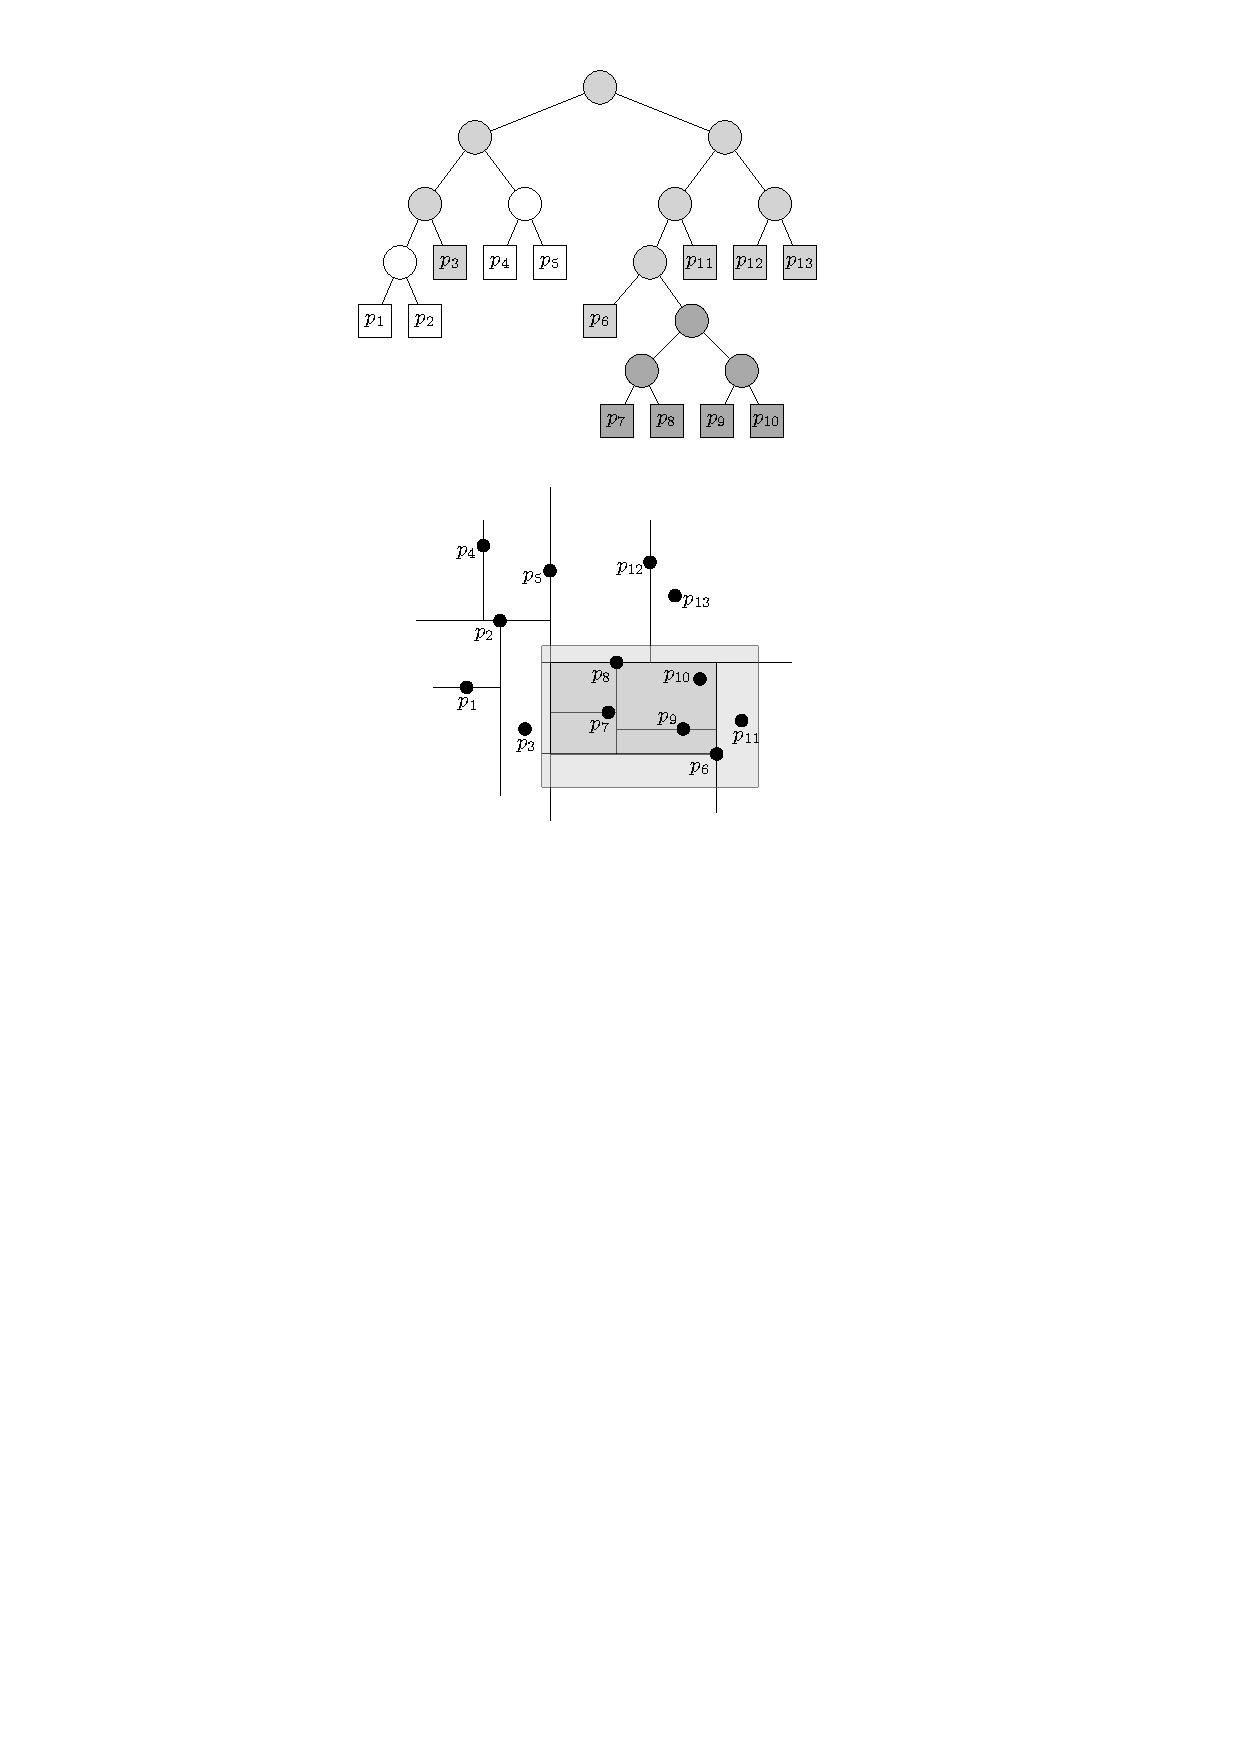
\includegraphics[scale=1.2]{pics/kdTree4.pdf}}		
\caption{Dvodimenzionalno kd drevo.}		
\label{kd-primer}		
\end{figure}
Kd drevo je podatkovna struktura za organizacijo $k$-dimenzionalnih točk z razbitjem prostora. Najpogosteje se uporablja za območna iskanja in iskanja najbližjih sosedov.
Kd drevo je v osnovi $k$-dimenzionalno binarno drevo, kjer vsako notranje vozlišče razdeli prostor na dva polprostora, ki ju ločuje hiperravnina. Pri $k=2$ gre za polravnini, ki ju ločuje premica. Točke levo od hiperravnine so vsebovane v levem poddrevesu vozlišča, točke desno od hiperravnine pa v desnem poddrevesu. Smer hiperravnine je odvisna od tega, po kateri dimenziji vozlišče razdeli prostor.
Za i-ti nivo drevesa velja, da je hiperravnina, ki razdeli prostor, pravokotna na koordinatno os, ki predstavlja $j = ((i-1)\mod k + 1)$-to dimenzijo prostora. Vozlišče na drugem nivoju dvodimenzionalnega kd drevesa tako razdeli
ravnino s premico, ki je vzporedna abscisni osi. Točke v spodnji polravnini se nahajajo v levem poddrevesu vozlišča, točke v zgornji polravnini pa v desnem poddrevesu. Hiperravnina, ki jo predstavlja neko vozlišče $v$ v $i$-tem nivoju,
gre skozi tisto točko, čigar $j$-ta koordinata predstavlja mediano v množici vseh točk, ki se nahajajo v drevesu s korenom. Točke so shranjene v listih drevesa.

Časovna zahtevnost izgradnje drevesa je $\OO(n\log n)$ (na vsakem nivoju drevesa je potrebno izračunati mediano, kar vzame $\OO(n)$ časa), prostorska zahtevnost drevesa pa je $\OO(n)$~\cite[poglavje~5.2]{bkos-08-all}.
\subsection{Območne poizvedbe}
Časovna zahtevnost območne poizvedbe je $\OO(n^{1-\frac{1}{d}} + k)$, kjer je $k$ število poročanih točk, $d$ pa dimenzija drevesa. V splošnem za dvodimenzionalno kd drevo velja, da je območje $\operatorname{reg}(v)$, ki ga predstavlja vozlišče $v$, pravokotnik, ki je lahko neomejen z več strani. Omejen je s hiperravninami (premicami), shranjenih v starših vozlišča $v$. Točka je vsebovana v poddrevesu s korenom $v$, če je vsebovana v $\operatorname{reg}(v)$. Poddrevo s korenom $v$ med poizvedbo obiščemo le, če poizvedbeno območje (pravokotnik) seka $\operatorname{reg}(v)$. Če
je $\operatorname{reg}(v)$ v celoti vsebovana v poizvedbenem območju, v rezultat dodamo vse točke v poddrevesu $v$. Če pridemo do lista, preverimo, ali je vozlišče shranjeno v njem vsebovano v območju. Primer poizvedbe je prikazan na sliki ~\ref{kd-primer} (pri čemer je treba opozoriti, da pri drevesu na sliki za razdelitev prostora ni bila vedno izbrana mediana).

\subsection{Kd drevesa v CGAL-u}
Implementacija podatkovne strukture dosledno sledi njenemu teoretičnemu opisu. Za območne poizvedbe je uporabljen standarden algoritem, ki rekurzivno preišče drevo. Implementiran je v funkciji \textit{search}, ki se nahaja v razredu \textit{Kd\U tree}. Poleg območnih so na voljo tudi poizvedbe za $k$ najbližjih ali $k$ najbolj oddaljenih točk, ki so implementirane v razredu \textit{Ortho\-go\-nal\U k\U neigh\-bor\U search}. 

\section{Območna drevesa}
Območna drevesa so še ena podatkovna struktura za območne poizvedbe. V nadaljevanju opisa se bomo omejili samo na dvodimenzionalna drevesa. V primerjavi s kd drevesi imajo boljši čas poizvedbe ($\OO(\log^2 n + k)$), ampak slabšo prostorsko zahtevnost ($\OO(n\log n)$). Namesto, da razdelimo prostor izmenično po abscisni in ordinatni osi, imamo tukaj kot glavno drevo uravnoteženo dvojiško iskalno drevo $\T$, zgrajeno nad prvimi koordinatami točk (koordinatami $x$). Vsako vozlišče $v$ drevesa ima potem kazalec na uravnoteženo dvojiško iskalno poddrevo $\T_{assoc}(v)$, zgrajeno nad drugimi ($y$) koordinatami točk, ki so shranjene v listih poddrevesa v $\T$ s korenom $v$. Primer drevesa je prikazan na sliki~\ref{range-primer}. 
Dejanske točke so shranjene v drevesih $\T_{assoc}(\cdot)$. Na danem nivoju drevesa $\T$ je neka točka $p \in P$ shranjena v natanko enem drevesu $\T_{assoc}(\cdot)$. Iz tega sledi, da vsa drevesa $\T_{assoc}(\cdot)$ na poljubnem nivoju drevesa $T$ porabijo skupaj $\OO(n)$ prostora. Ker je globina drevesa $\T$ reda $\OO(\log n)$, je prostorska zahtevnost območnih dreves $\OO(n\log n)$.

\begin{figure}
\centerline{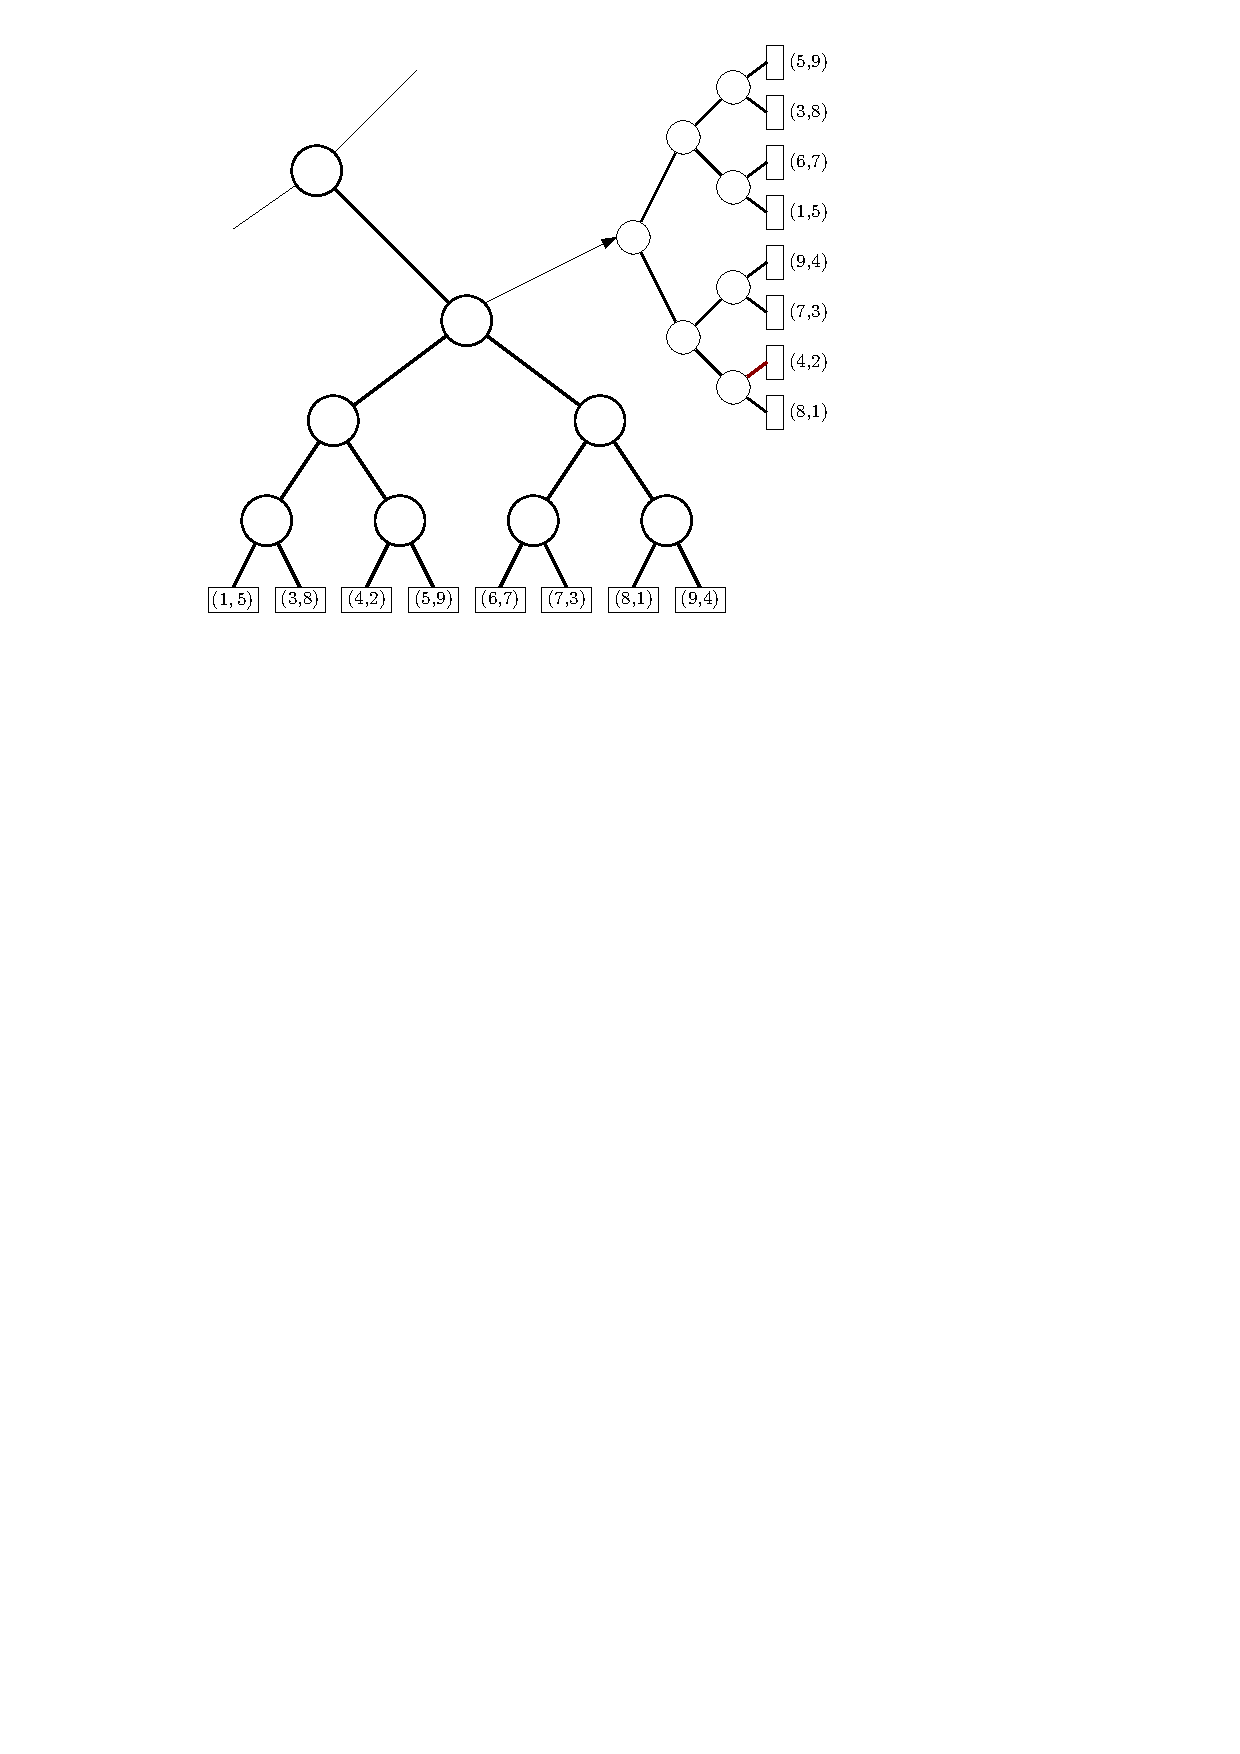
\includegraphics[scale=1]{pics/rangeTree2.pdf}}
\caption{Dvodimenzionalno območno drevo.}
\label{range-primer}
\end{figure}

\subsection{Poizvedbe}
Naj bo $P(u)$ poddrevo območnega drevesa, ki ima za koren vozlišče $u$. Poizvedba $[x,x'] \times [y,y']$ poteka na sledeč način. V glavnem drevesu iščemo z intervalom $[x,x']$, dokler ne pridemo do vozlišča $v_{split}$, kjer se iskanje razcepi na dva dela. Iskanje nadaljujemo v smeri njegovega levega otroka in pri vsakem obiskanem vozlišču $v$, kjer se pot iskanja nadaljuje levo, označimo njegovega desnega otroka. Podobno nadaljujemo v smeri desnega otroka vozlišča $v_{split}$ in označimo levega otroka obiskanega vozlišča $v$, pri katerem se iskanje nadaljuje v desno. 
V tem trenutku imamo označenih $\OO(\log n)$ poddreves. Za vsako poddrevo $P(v)$ naredimo poizvedbo $[y,y']$ na sekundarnem drevesu $\T_{assoc}(v)$, ki hrani vse točke iz $P(v)$. 

Časovna zahtevnost enodimenzionalne poizvedbe v poddrevesu $\T_{assoc}(v)$ je $\OO(\log n + k_v)$, kjer je $k_v$ število vrnjenih točk. Celotni čas poizvedbe je $\sum_v\OO(\log n + k_v)$, torej vsota vseh obiskanih vozlišč v $T$. Ker je dolžina obeh iskalnih poti (ki se razcepita pri vozlišču $v_{split}$) enaka $\OO(\log n)$, in je vsota $\sum_v k_v$ enaka številu vseh vrnjenih točk poizvedbe $k$, je časovna zahtevnost celotne poizvedbe $\OO(\log^2n + k)$~\cite[poglavje 5.3]{bkos-08-all}.

\subsection{Območna drevesa v CGAL-u}
Vhodni podatkovni tip za $d$-dimenzionalno območno drevo je zbirka, ki vsebuje podatkovni tip za $d$-dimenzionalno točko in po želji tip vrednosti, s katerim lahko shranimo poljubni podatek. Primer uporabe slednjega bi lahko bila množica točk, ki sestavljajo več večkotnikov. Vsako vozlišče drevesa bi potem kot ključ shranilo neko točko, kot vrednost pa poligon, kateremu ta točka pripada. 

Razred za območno drevo je popolnoma generičen, kar pomeni, da z njim lahko definiramo večnivojska drevesa. $d$-dimenzionalno večnivojsko drevo  (z $d$ nivoji) je na $d$-tem nivoju preprosto drevo, na $k$-tem nivoju, $1 \leq k \leq d-1$, pa drevo, kjer vsako notranje vozlišče vsebuje večnivojsko drevo dimenzije $d-k+1$. $k-1$-dimenzionalno drevo, ki je vgnezdeno drevo v $k$-dimenzionalnem drevesu \T, imenujemo podnivojsko drevo drevesa \T. 


Razred je neodvisen tako od vrste podatkov kot od njihove konkretne predstavitve. Za tako splošnost moramo definirati, kako je predstavljeno drevo na vsakem nivoju in kako so vhodni podatki organizirani. Drevesa z dimenzijo $k$, $ 1 < k < 4$, so zato v CGAL-u definirana v lastnih razredih, pripravljenih za takojšnjo uporabo. Ko je drevo enkrat zgrajeno, dodajanje ali brisanje podatkov iz njega ni več mogoče.

\bigbreak
Drevo je parametrizirano s tremi predlogami: podatki, oknom in geometrijskimi značilnostmi. Prvi definira vrsto podatkov, drugi poizvedbeno območje, tretji pa podajajo implementacijo metod, ki jih drevo uporablja za dostop do podatkov. Da bi se izognili uporabi vgnezdenih predlog za argumente (do česar pride, če bi drevo na vsakem nivoju imelo predlogo za tip poddrevesa), so drevesa definirana s pomočjo objektnega programiranja. CGAL je definiral virtualni bazni razred \textit{Tree\U base}, iz katerega je izpeljan razred \textit{Range\U tree\U d}. Konstrukturju slednjega moramo kot argument podati prototip poddrevesa tipa \textit{Tree\U base}, ki je lahko zopet objekt razreda \textit{Range\U tree\U d}. Za zaustavitev rekurzije je iz \textit{Tree\U base} izpeljan še razred \textit{Tree\U anchor}, čigar konstruktor ne pričakuje nobenega argumenta. Tako opisana konstrukcija sledi modelu prototipa in v njej je poddrevo sicer definirano s pomočjo objektnega programiranja v času izvajanja programa, kar pa predstavlja zanemarljiv časovni strošek.

\section{Delaunayeva triangulacija}
Delaunayeva triangulacija (DT) nad točkami $P$ je triangulacija $DT(P)$, ki izpolnjuje Delaunayev pogoj. Ta pogoj pravi, da se nobena točka iz $P$ ne nahaja znotraj poljubnemu trikotniku očrtanega kroga triangulacije. Taka triangulacija
maksimizira minimalni kot med vsemi koti trikotnikov triangulacije. Množica $P$ s kolinearnimi točkami predstavlja izrojen primer, za katerega ne obstaja nobena Delaunayeva triangulacija. Če štiri točke v $P$ ležijo na isti krožnici, rešitev ni enolična.

Med točko $p$ in njenim najbližjim sosedom $q$, kjer $p,q\in P$, vedno obstaja povezava $pq\in E(DT(P))$, ker je graf najbližjih sosedov nad množico $P$ podgraf Delaunayeve triangulacije. Za dolžino najkrajše poti $d_{DT(P)}(\pi (p,q))$ med dvema 
vozliščema $p,q$ v Delaunayevi triangulaciji velja:

\begin{equation*}
d_{DT(P)}(\pi (p,q)) \le 1.998\times d_{DT(P)}(p,q)~\cite{DT1998}
\end{equation*}

Za izgradnjo Delaunayeve triangulacije poznamo več algoritmov. Najpogosteje uporabljeni so: 

\begin{description}
\item[Algoritem z obračanjem.] Pomembna lastnost dveh trikotnikov ABD in BCD s skupno stranico BD v Delaunayevi triangulaciji je, da je vsota kotov $\alpha$ in $\gamma$ manjša od 180\textdegree (glej sliko~\ref{dt-triangle}). Če ta lastnost ne velja, jo lahko dosežemo z obračanjem trikotnikov, tako da dobimo trikotnika ABC in ACD s skupno stranico AC. Algoritem z obračanjem zgradi navadno triangulacijo, nato pa izvaja operacijo obračanja, dokler vsi trikotniki ne izpolnjujejo Delaunayevega pogoja. Časovna zahtevnost v najslabšem primeru je $\OO(n^2)$.
\item[Inkrementalni algoritem z vstavljanjem.] Dodaja točke zaporedoma v obstoječo triangulacijo. Ko je nova točka dodana, se tiste dele Delaunayevega grafa, na katere nova točka vpliva, popravi z obračanjem trikotnikov. V najslabšem primeru je časovna zahtevnost algoritma $\OO(n^2)$, ker moramo za vsako dodano točko najti trikotnik, ki jo vsebuje ($\OO(n)$), in popraviti vse trikotnike ($\OO(n)$). Z nekoliko izboljšanim algoritmom za iskanje lokacije nove točke je pričakovana časovna zahtevnost $\OO(n\log n)$, ker je v povprečju v vsakem koraku obrnjenih $\OO(1)$ trikotnikov, iskanje lokacije nove točke pa vzame v povprečju $\OO(\log n)$ časa.
\item[Deli in vladaj.] Točke so rekurzivno razdeljene s premico v dve množici podobne moči. Delaunayeva triangulacija je izračunana za vsako množico točk posebej, nato pa sta obe triangulaciji združeni vzdolž premice. Združevanje vzame $\OO(n)$ časa, tako da je časovna zahtevnost algoritma $\OO(n\log n)$. V praksi je deli in vladaj najhitrejši algoritem za izgradnjo Delaunayeve triangulacije.
\end{description}

\begin{figure}
\centerline{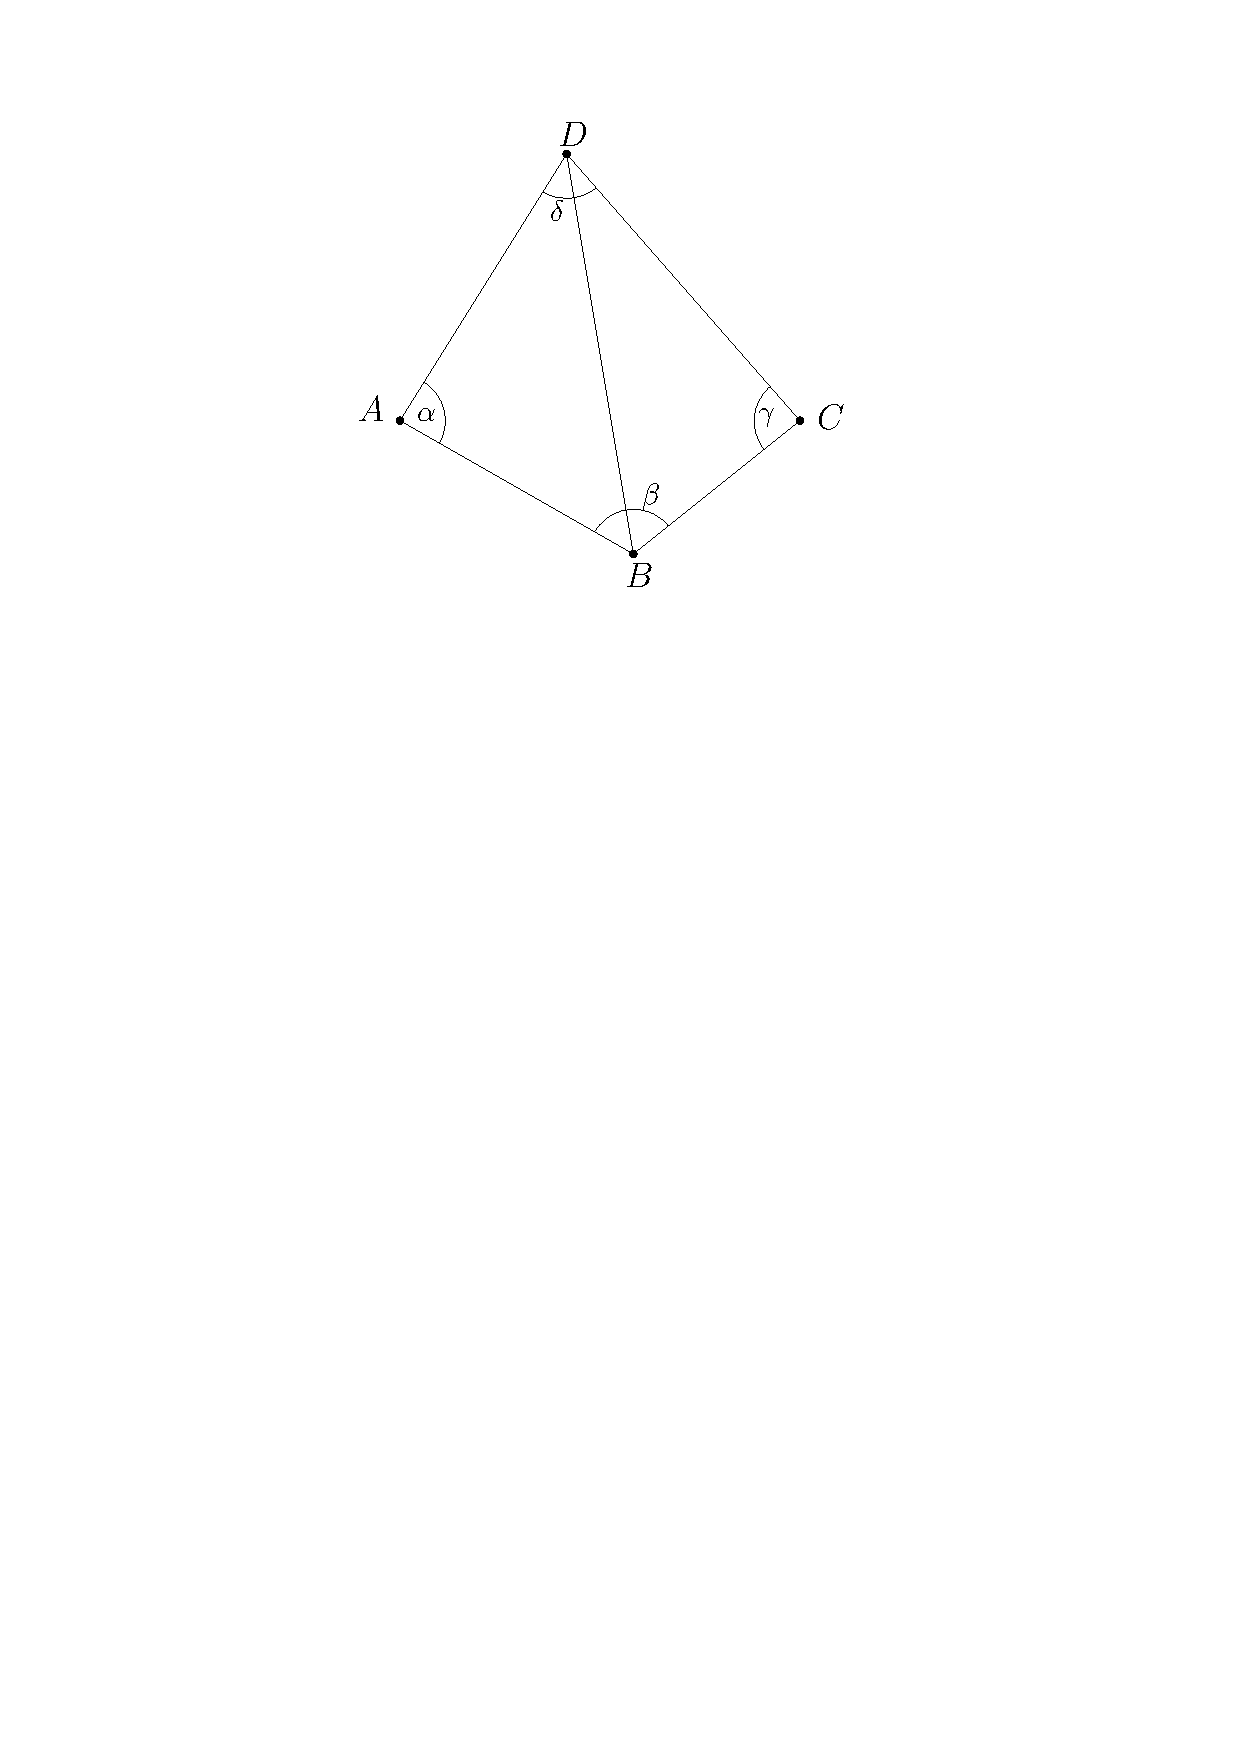
\includegraphics[scale=0.8]{pics/dt-triangle.pdf}}
\caption{Primer trikotnikov, ki ne izpolnjujeta Delaunayevega pogoja. Z metodo obračanja lahko povezavo BD zamenjamo s povezavo AC, s čimer je pogoj izpolnjen.}
\label{dt-triangle}
\end{figure}

\subsection{Delaunayeva triangulacija v CGAL-u}
Razred Delaunay\U triangulation\U 2 implementira DT in deduje iz razreda Triangulation\U 2. Iz slednjega uporablja nekatere metode, kot so vstavljanje ali določanje položaja točke, nekatere pa tudi povozi, kot je recimo obračanje trikotnikov, ker trikotnikom v navadni triangulaciji ni potrebno izpolnjevati Delaunayevega pogoja. Poleg tega vsebuje dodatne metode za iskanje najbližjega soseda in izgradnjo elementov Voronoijevega diagrama, dualnega DT-ju.

Razred je parametriziran z dvema predlogama. Prvi je razred geometrijskih značilnosti, drugi pa razred podatkovne strukture za triangulacijo. Za slednjega CGAL ponuja privzeti razred \textit{ Triangulation\U data\U structure\U 2}, ki vsebuje zbirki vozlišč in lic. Razred geometrijskih značilnosti mora biti model koncepta \textit{DelaunayTriangulationTraits\U 2}, ki je dodelana verzija koncepta \textit{TriangulationTraits\U 2}. Ta vsebuje predikata za primerjavo koordinat dveh točk in test orientacije treh točk. \textit{DelaunayTriangulationTraits\U 2} dodatno vsebuje še predikat \textit{side\U of\U oriented\U circle}, ki za štiri dane točke $p, q, r, s$ določi položaj točke $s$ glede na krožnico, ki gre skozi točke $p, q$ in $r$.

Implementacija izgradnje triangulacije uporablja inkrementalni algoritem z obračanjem~\cite{cgal:y-t2-16b}.

\subsubsection{Operacije nad strukturo}
\begin{description}
\item[Določanje položaja točke.] Je implementirano s sprehodom po povezavah. Sprehod se začne pri vozlišču podanega lica, ali pri naključnem vozlišču, če lice ni podano. Za naključno vozlišče je povprečna časovna zahtevnost $\OO(\sqrt{n})$.
\item[Vstavljanje nove točke.] Najprej je uporabljena metoda \textit{locate} za določanje položaja lica, ki vsebuje novo točko, nato pa se lice razbije na tri dele. Novo triangulacijo se nato popravi z $\OO(d)$ obračanji (v povprečju $\OO(1)$), kjer je $d$ stopnja novega vozlišča triangulacije
\item[Iskanje najbližjega soseda.] Uporabljena je metoda \textit{locate}, ki potrebuje $\OO(1)$ časa pri enakomerno porazdeljenih vozliščih, v najslabšem primeru pa $\OO(n)$ časa.
\end{description}

\subsubsection{Hierarhija triangulacij}
Za učinkovito določanje položaja točk lahko uporabimo razred \textit{Trian\-gu\-la\-tion\U hier\-archy\U 2}, ki hrani hierarhijo triangulacij. Na najnižjem nivoju se nahaja izvirna triangulacija, nad katero se izvajajo operacije in lociranje točk. Na vsakem višjem nivoju je nato zgrajena triangulacija nad manjšo množico naključno izbranih vozlišč iz triangulacije na predhodnem nivoju (recimo 3\% vozlišč). Določanje položaja točke se izvede od zgoraj navzdol po strukturi: na najvišjem nivoju se naivno izvede poizvedba najbližjega soseda, nato pa se na vsakem naslednjem nivoju najbližjega soseda poišče s sprehodom po povezavah z začetkom pri najbližjem sosedu v triangulaciji na višjem nivoju. Taka struktura je najbolj primerna ravno za DT. Poleg hitrega delovanja na realnih podatkih ima dobro časovno zahtevnost v najslabšem primeru in nizko prostorsko zahtevnost~\cite{Olivier}.

\section{Voronoijev diagram}
\begin{figure}
\centerline{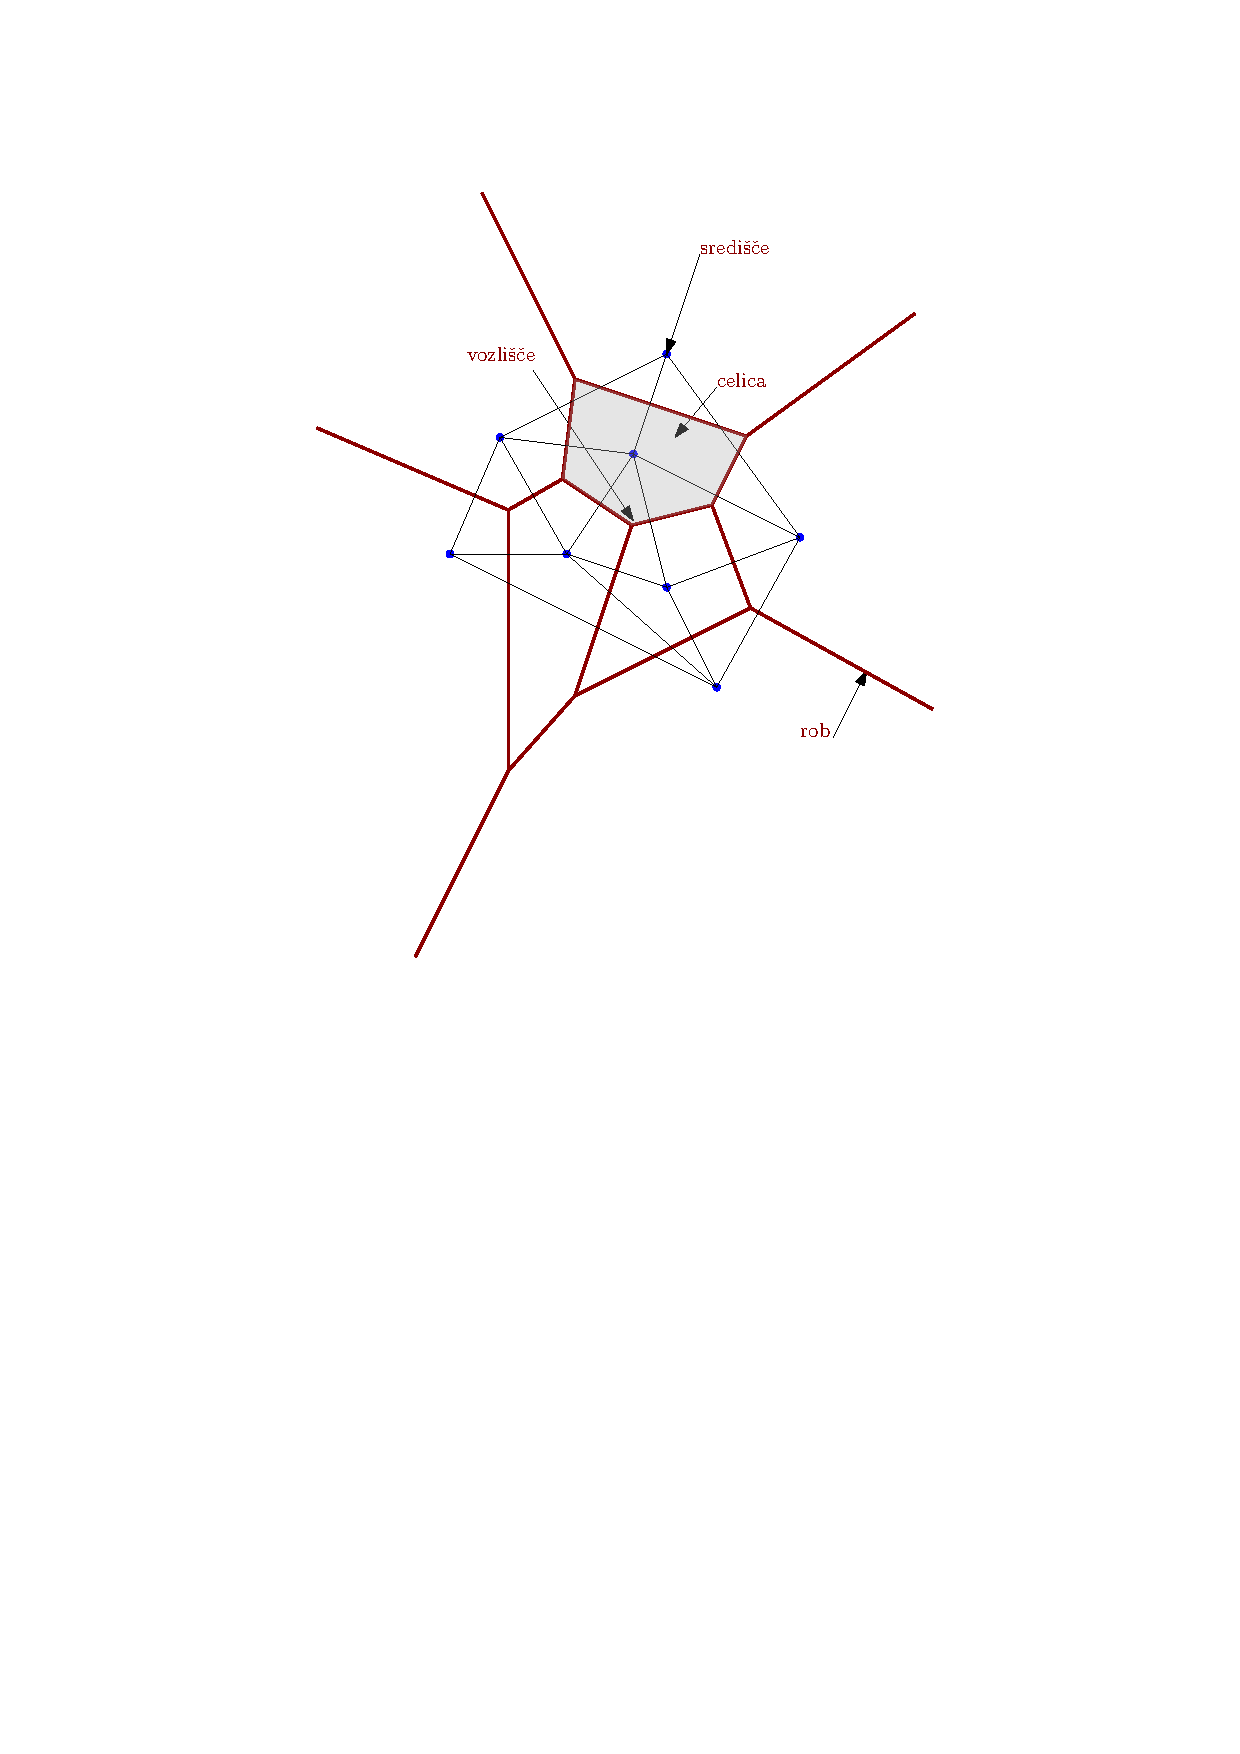
\includegraphics[scale=0.8]{pics/voronoi-dt3.pdf}}
\caption{Evklidski Voronoijev diagram, označen z rdečimi odebeljenimi povezavami. Voronoijeva središča, obarvana z modro barvo, predstavljajo hkrati tudi vozlišča v Delaunayevi triangulaciji (dualni VD-ju), ki je označena s tanjšimi črnimi povezavami.}
\label{vd}
\end{figure}

Voronoijev diagram (VD) je definiran na množici točk, imenovanih Voronoijeva središča (angl. $sites$), in z metriko oziroma funkcijo razdalje med točkami.

Naj bo $S = \{S_1,S_2,...,S_n\}$ množica Voronoijevih središč in naj bo $\delta(x,S_i)$ funkcija razdalje med središčem $S_i$ in neko točko $x \in \mathbb{R}^2$. Množica točk $V_{ij}$, ki so bližje središču $S_i$ kot središču $S_j$ na podlagi funkcije $\delta(x,\cdot)$, je množica:

\begin{equation*}
V_{ij} = \{x \in \mathbb{R}^2: \delta(x,S_i) < \delta(x,S_j)\}. 
\end{equation*}

Množico $V_i$ točk, ki so bližje središču $S_i$ kot kateremu koli drugemu središču, lahko potem definiramo kot množico:

\begin{equation*}
V_i = \bigcap_{j \neq i} V_{ij} .
\end{equation*}

Množico $V_i$ imenujemo tudi Voronoijeva celica ali Voronijevo lice središča $S_i$. Množica točk, ki so enako oddaljene od dveh najbližjih središč, predstavlja Voronijev bisektor. Povezani podmnožici slednjega pravimo Voronoijev rob. Točki, ki je enako oddaljena od treh ali več najbližjih središč, pravimo Voronoijevo oglišče. Voronoijev diagram na množici $S$ in z metriko $\delta(x,\cdot)$ je zbirka Voronoijevih celic, robov in vozlišč ter je podoben ravninskemu grafu.

Celice si ponavadi predstavljamo kot 2-dimenzionalne, robove kot 1-dimen\- zionalne in vozlišča kot 0-dimenzionalne objekte. Za določene kombinacije središč in metrik to ne drži. Voronoijev diagram z metriko $L_1$ ali $L_{\infty}$ lahko na primer vsebuje dvodimenzionalne robove. Takim Voronoijevim diagramom, za katere zgornja omejitev drži in imajo lastnost, da so njihove celice preprosto povezano območje v ravnini, pravimo preprosti Voronoijevi diagrami. Najbolj tipičen primer slednjih je evklidski Voronoijev diagram (slika ~\ref{vd}), ki ga uporabljamo v našem algoritmu.

\subsection{Voronoijev diagram v CGAL-u}
Knjižnica CGAL vsebuje razred \textit{Voronoi\U diagram\U 2}, ki deluje kot prilagoditveni paket. Slednji na podlagi podanih kriterijev prilagodi DT pripadajočemu VD-ju, ki je predstavljen kot struktura DCEL (angl. \textit{doubly connected edge list}). Paket je torej zasnovan tako, da na zunaj deluje kot struktura DCEL, znotraj pa v resnici hrani strukturo grafa, ki predstavlja graf Delaunayeve triangulacije.

Razred je parametriziran s tremi predlogami. Prvi, $DG$, mora biti model koncepta razreda \textit{DelaunayGraph\U 2}. Primeri takih struktur so DT, navadna triangulacija, Apollonov graf in hierarhija triangulacij. Druga predloga, $AT$, predstavlja lastnosti pretvorbe DT v VD ter definira tipe struktur in funktorje, ki jih razred potrebuje za dostop do geometrijskih lastnosti DT-ja. Funktor mora biti recimo definiran za izgradnjo Voronoijevih vozlišč iz njihovih dualnih lic v DT. Pomemben je tudi funktor za poizvedbe najbližjih središč, ki kot rezultat vrne informacijo o tem, koliko in katera središča so enako oddaljena od točke poizvedbe. Bolj konkretno, rezultat je Delaunayevo vozlišče, lice ali rob, na katerem točka poizvedbe leži oziroma z njim sovpada. Če je na primer točka poizvedbe $q$, enako oddaljena od treh središč, potem sovpada z nekim Voronoijevim vozliščem, zato funktor vrne Delaunayevo lice, ki je dualno temu vozlišču. Razred, ki predstavlja Delaunayevo lice, omogoča iteracijo po Delaunayevih vozliščih, ki definirajo lice, ta pa so dualna trem Voronoijevim središčem.

Tretja predloga predstavlja režim prilagoditve DT-ja VD-ju. 
Če množica središč, ki določa graf DT-ja, vsebuje podmmnožice središč, ki so v izrojenem položaju, ima dualni graf - VD - lahko robove z dolžino nič in po možnosti tudi celice s ploščino nič. Režim prilagoditve določa, kaj storiti v takih primerih. V našem projektu smo uporabili režim \textit{Delaunay\U triangulation\U ca\-ching\U de\-ge\-ne\-ra\-cy\U re\-mo\-val\U po\-licy\U 2}. Kot pove že ime, ta tip poskrbi, da so vse zgoraj opisane celice in robovi odstranjeni iz VD. Poleg tega uporablja predpomnilnik pri ugotavljanju, ali ima določena celica oziroma rob degenerirane lastnosti. Ker je slednje precej zahtevna operacija, se ta tip izplača pri vhodnih podatkih (središčih) z veliko izrojenimi primeri ~\cite{cgal:k-vda2-15a}.






\chapter{Teoretični opis algoritmov}
Naj bo $P$ množica točk, ki predstavljajo središča krogov $\D$. Množica $P$ predstavlja vhod našega algoritma in vse operacije ter uporabljene podatkovne strukture se vrtijo okrog te množice. Kardinalnost množice je enaka $n$.

\begin{figure}
\centerline{\includegraphics[scale=0.6,page=4]{pics/unitdisks.pdf}}
\caption{Slikovna predstavitev problema. Točki $s$ in $t$ ločuje množica krogov, definiranih z njihovimi središči.}
\label{separation}
\end{figure}

\begin{figure}
\centerline{\includegraphics[scale=0.6,page=5]{pics/unitdisks.pdf}}
\caption{Graf $G(P)$, zgrajen nad množico $P$ v sliki ~\ref{separation}.}
\label{gdisks}
\end{figure}

Naj bo $G(P)$ graf z množico vozlišč $P$ in s povezavo med točkama $p,q \in P$, če velja $|pq|\le 1$, kjer je uporabljena evklidska metrika (glej sliko~\ref{gdisks}). Vse povezave so neutežene. V nadaljevanju bomo namesto $G(P)$ pisali preprosto $G$.
\section{Drevo najkrajših poti v grafu enotskih krogov}
\subsection{Eksplicitna uporaba preiskovanja v širino (BFS)}
\label{bfs-theory}

Najenostavnejši način izgradnje drevesa najkrajših poti nad množico točk $P$ je uporabiti preiskovanje v širino nad grafom $G$. V vrsti hranimo še ne obiskane točke, ki so sosedne že obiskanim (na začetku je to izbrani koren). Vsaki točki, ki jo obiščemo, nastavimo za starša sosedno točko, prek katere smo do nje prišli, in ji nastavimo razdaljo, ki je za 1 večja od razdalje njenega starša. Prav tako jo označimo kot obiskano točko in s tem preprečimo, da bi neko točko dodali v vrsto več kot enkrat. Psevdokoda algoritma je prikazana na sliki~\ref{fig:genericBfs}. 
\begin{figure}[htp]
\begin{center}
\ovalbox{~~~~
\begin{varwidth}{\linewidth}
\begin{codebox}
    \Procname{$\proc{BFS}(G,s)$}
    \li // za vsako povezavo $e\in E(G)$ velja $dist(e) \leq 1$ 
    \li \For $u\in V(G) - \{s\}$ \Do
    	\li $u.visited \gets$ false
    	\li $u.dist \gets \infty$
    	\li $u.\pi \gets \const{nil}$
    \End
    \li $s.visited =$ true
    \li $u.dist = 0$
    \li $u.\pi = \const{nil}$
    \li $Q$ je prazna vrsta
    \li enqueue($Q, s$)
    \li \While $Q \neq \emptyset$ \Do
    	\li $u =$ dequeue($Q$)
    	\li \For $(u,v) \in G.E$ \Do
    		\li \If $v.visited =$ false \Do
    			\li $v.visited =$ true
    			\li $v.dist = u.dist + 1$
    			\li $v.\pi = u$
    			\li enqueue($Q, v$)
    		\End
    	\End
	\End
    \\[-2mm]
\end{codebox}
\end{varwidth}
~~~~}\end{center}
\caption{Psevdokoda eksplicitnega (splošnega) algoritma za izgradnjo drevesa najkrajših poti s preiskovanjem v širino.}
\label{fig:genericBfs}
\end{figure}
Očitna slabost algoritma je nujnost izgradnje grafa $G$, ki ima časovno zahtevnost $\OO(n^2)$ v najslabšem primeru. Časovna zahtevnost izgradnje drevesa najkrajših poti je $\OO(n + |E|)$, kjer $|E|$ predstavlja število povezav v grafu. To pomeni, da je izgradnja drevesa časovno odvisna od gostote grafa (ker povezave v grafu $G$ obstajajo samo med točkami z razdaljo največ 1), in v najslabšem primeru je čas izgradnje kvadratičen. Prednost uporabe algoritma s preiskovanjem v širino je enostavnost rešitve (in implementacije). V situacijah, kjer ima graf $G$ malo povezav in je vnaprej znan ali ga je treba izračunati v vsakem primeru, ima tak algoritem tudi očitno prednost pred ostalimi rešitvami. 

%\afterpage{\FloatBarrier}

\subsection{Preiskovanje v širino z uporabo kvadratne mreže (grid)}
%\afterpage{\FloatBarrier}
Graf enotske kvadratne mreže je lahko za preiskovanje v širino uporabljen kot alternativa klasičnemu algoritmu BFS nad grafom enotskih razdalj. Vsaki točki iz dane množice $P$ lahko izračunamo njen ključ tako, da poiščemo spodnje levo vozlišče celice grafa kvadratne mreže, v kateri se točka nahaja (glej sliko ~\ref{grid-fig}). Graf $G(P)$ lahko tako predstavimo s slovarjem, kjer ključi predstavljajo vozlišča grafa kvadratne mreže, kot vrednosti pa hranijo seznam vseh točk v celici, ki se nahaja zgoraj desno od ključa. Preiskovanje v širino nad takim grafom poteka tako, da za dano točko preverimo samo tiste kandidate, ki se nahajajo v isti ali eni izmed sosednjih celic grafa kvadratne mreže, točki pa povežemo, če je njuna razdalja največ 1.

\begin{figure}[htp]
\centerline{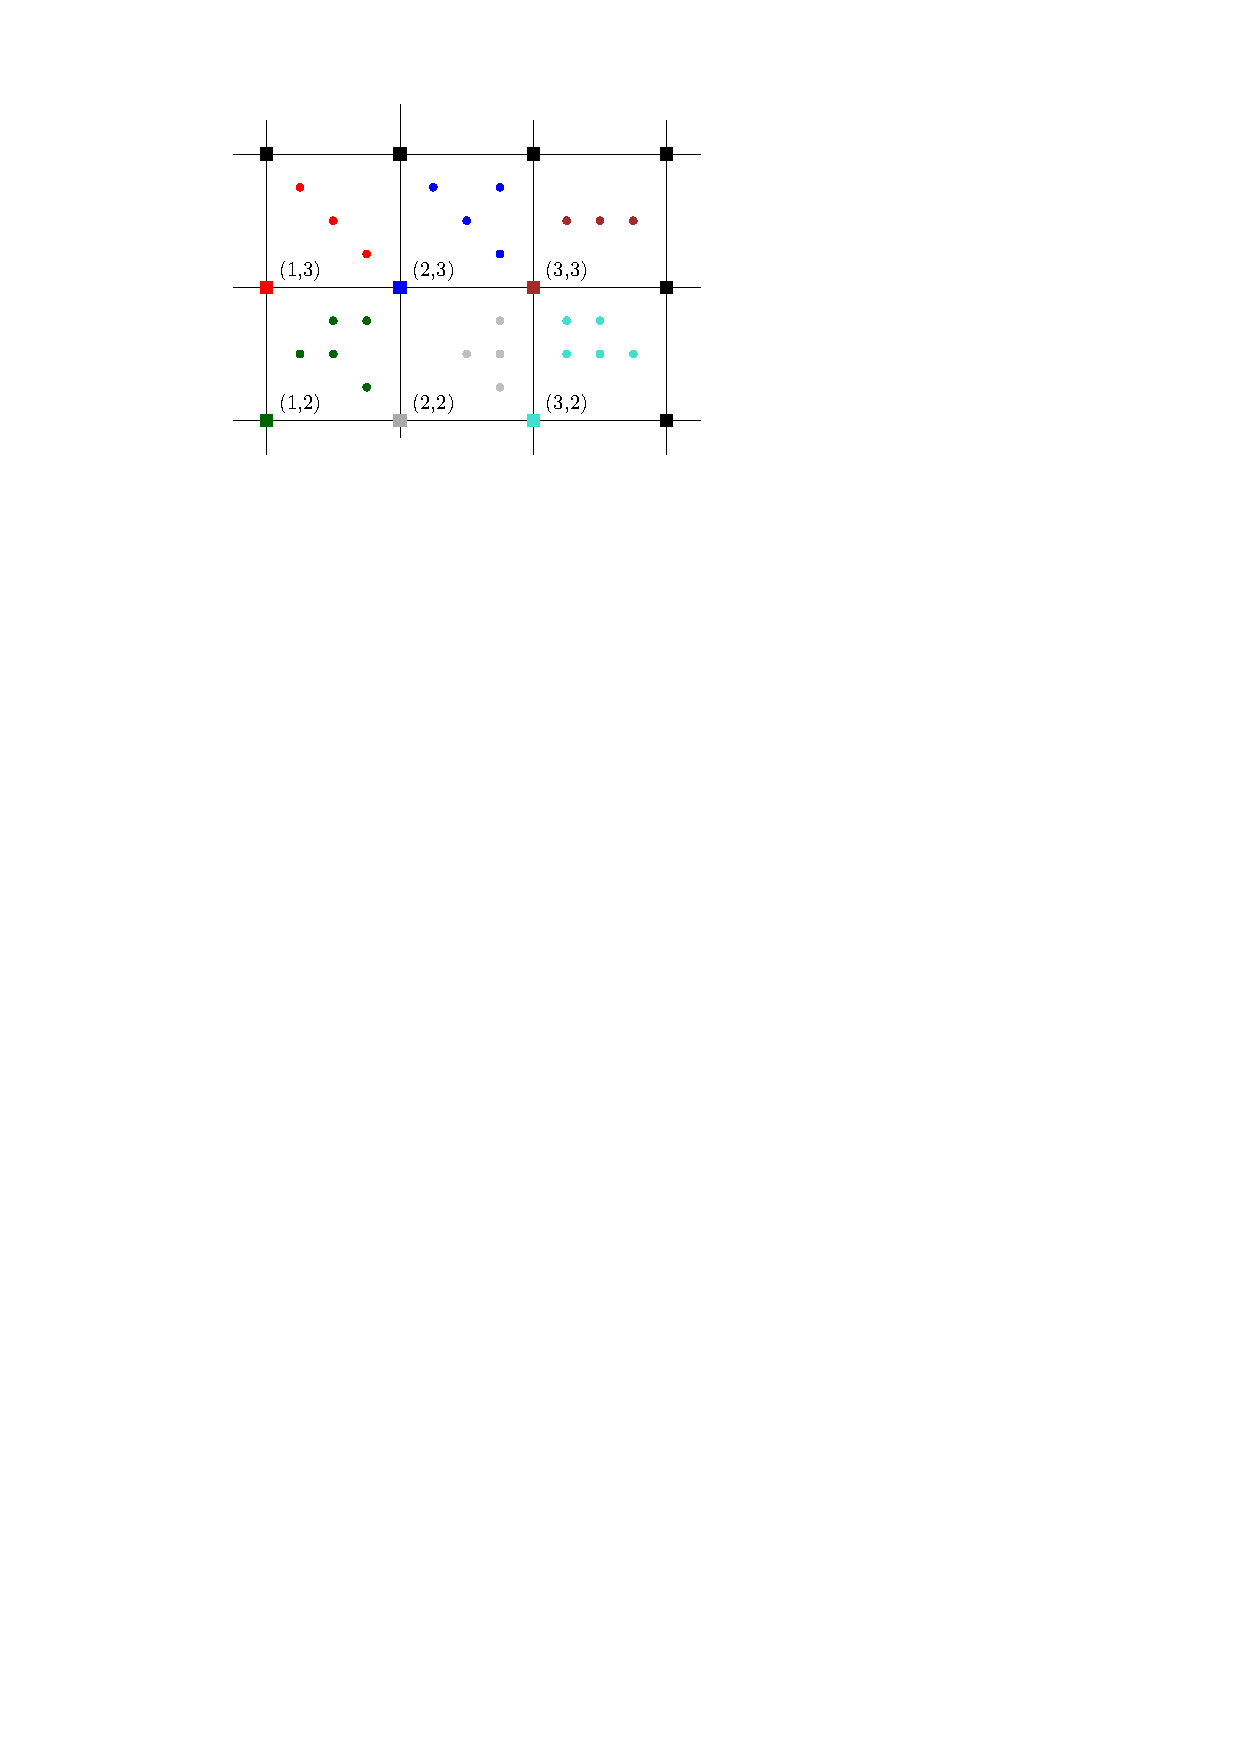
\includegraphics[scale=1.2]{pics/grid.pdf}}
\caption{Primer mrežnega grafa, v katerem do točk posamezne celice dostopamo prek vozlišča grafa (ključa), ki sovpada s spodnjim levim vozliščem celice. Točke so predstavljene z isto barvo kot njihov ključ.}
\label{grid-fig}
\end{figure}

Graf v taki obliki lahko zgradimo v linearnem času. Za vsako točko porabimo $\OO(1)$ časa, da izračunamo njen ključ in $\OO(1)$ časa, da jo vstavimo v seznam ključa. Ker graf med gradnjo drevesa najkrajših poti spreminjamo, ga moramo za vsako drevo zgraditi na novo. V tem smislu je od navadnega algoritma BFS bistveno hitrejši. Po drugi strani je tako kot pri BFS časovna zahtevnost izgradnje drevesa odvisna od porazdelitve točk. Večja kot je gostota točk, manj celic vsebuje točke oziroma je povprečje točk, ki jih posamezna celica vsebuje, višje.

\subsection{Prilagojen algoritem za enotske kroge (SSSP)}
\label{sssp-tree}

\begin{figure}[htp]
\centerline{\includegraphics[scale=0.6,page=6]{pics/unitdisks.pdf}}
\caption{Primer drevesa najkrajših poti z določenim korenom $r$ nad množico $P$ v sliki~\ref{separation}.}
\label{sssp-tree-ex}
\end{figure}

V tem poglavju je opisan algoritem za izgradnjo drevesa SSSP (ang. single source shortest path) iz~\cite{CJ15}. Gre za preiskovanje v širino nad grafom $G(P)$ brez dejanske izgradnje grafa. Vhod algoritma je torej $P$, pri izgradnji drevesa pa se uporablja abstrakten graf $G$. Primer drevesa je prikazan na sliki~\ref{sssp-tree-ex}.



Algoritem dobi kot vhod poleg množice $P$ izvorno točko $s\in P$ in nato inkrementalno v vsaki iteraciji dodaja točke h grafu. Množico točk, dodanih k drevesu v $i$-ti iteraciji, označimo kot
\[	W_i = \{ p\in P \mid d_{G}(s,p) = i\}.
	\]

Velja torej $W_0 = \{s\}$. Za izgradnjo $W_i$ ne potrebujemo celotnega grafa, zgrajenega do $i-1$-te iteracije, temveč samo množico $W_{i-1}$.  Za vsak $q\in W_i$ velja, da je povezan z natanko eno točko $p$ v množici $W_{i-1}$,  ki je izmed točk v $W_i$ najbližje $q$.

Pri izgradnji $W_i$ ne pregledujemo vseh še ne dodanih točk. Že v samem začetku najprej zgradimo $DT(P)$, ki nam je v pomoč pri iskanju primernih kandidatov za $W_i$. To so:

\begin{itemize}
\item točke, ki so sosedne $W_{i-1}$ v $DT(P)$, in
\item točke, ki so sosedne (do tega trenutka zgrajeni) $W_i$ v $DT(P)$.
\end{itemize} 

\begin{lema}
\label{lema1}
Naj bo $p$ točka v $P\backslash \{s\}$, za katero velja $d_G(s,p) < \infty$. Obstajata točka $w\in P$ in pot $\pi$ v $DT(P)$ od $w$ do $p$, za kateri velja $d_G(s,w)+1 = d_G(s,p)$ in $d_G(s,p_j) = d_G(s,p)$ za vsako notranje vozlišče $p_j$ v $\pi$.
\end{lema}

\begin{figure}[htp]
\centerline{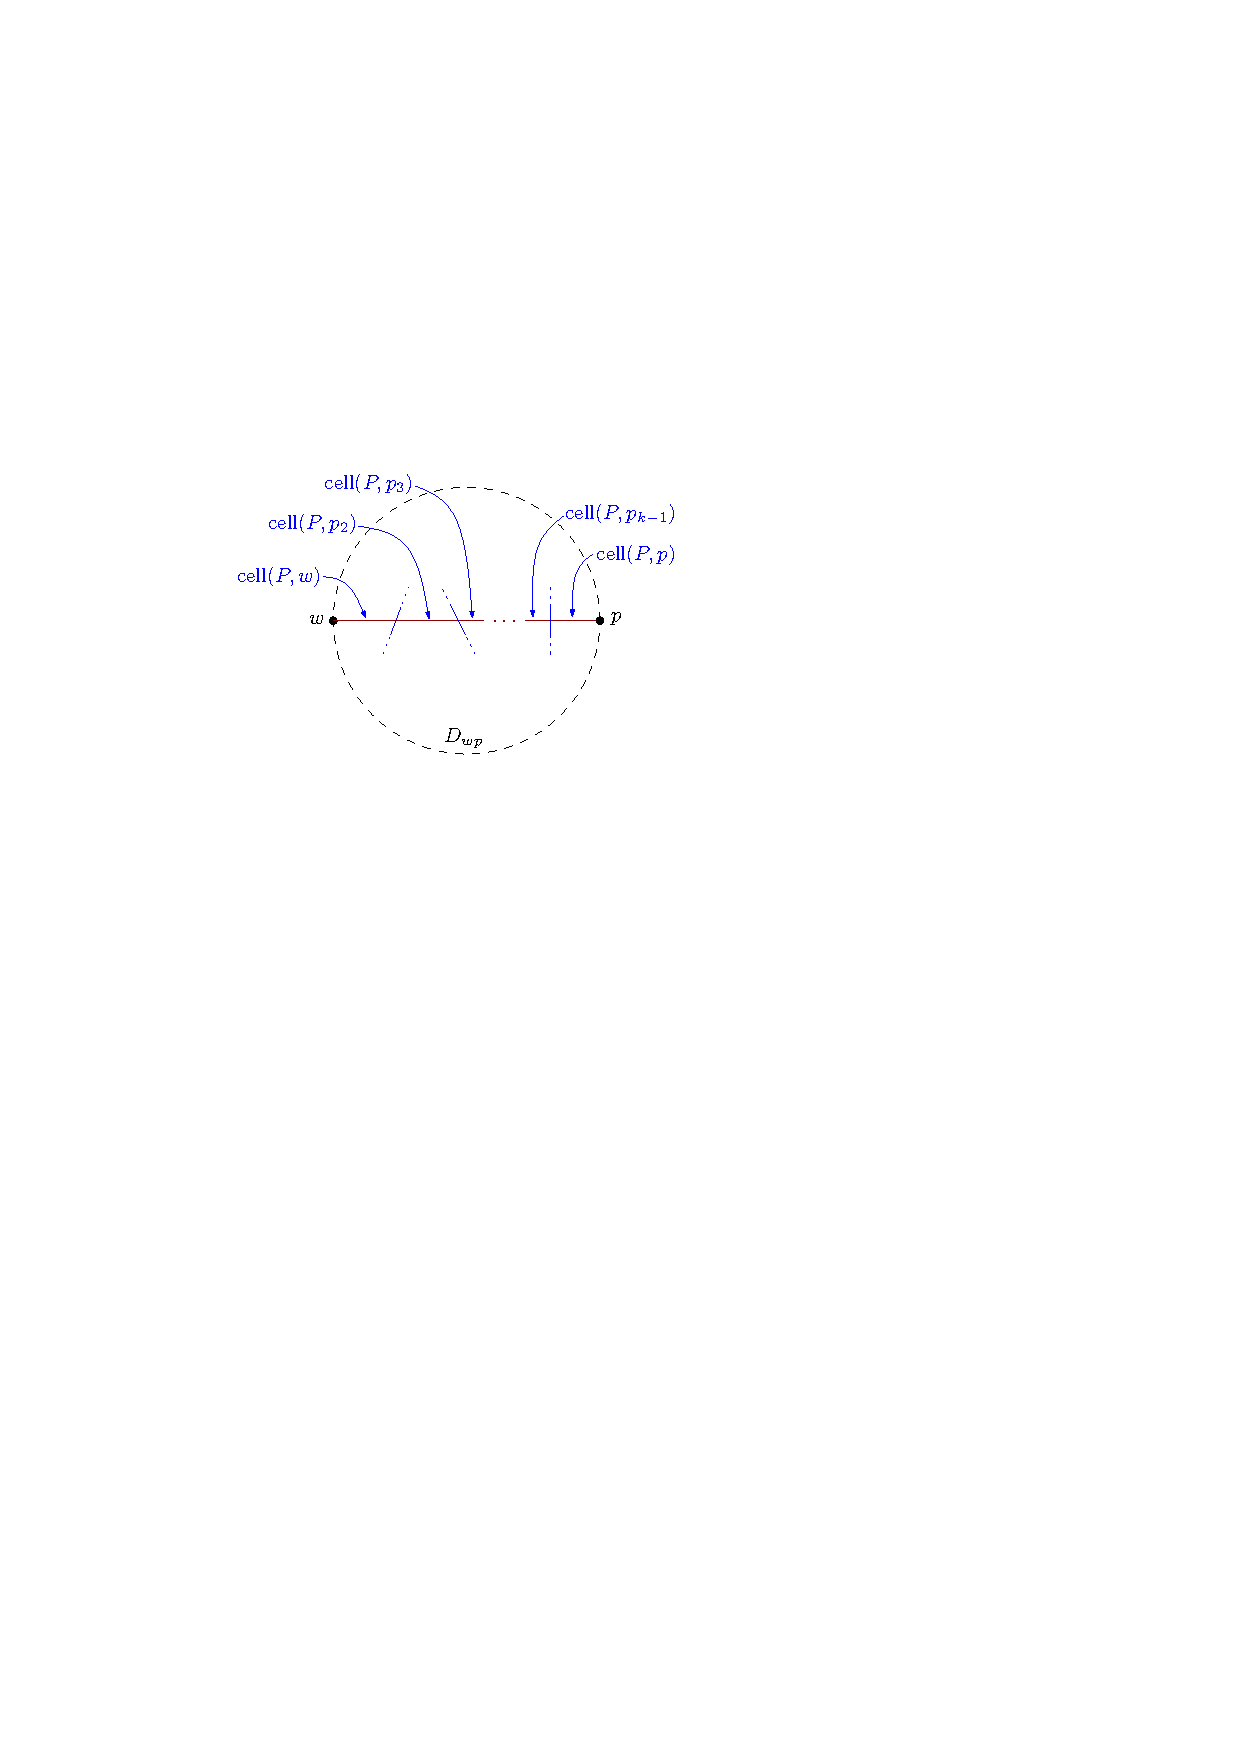
\includegraphics[scale=1]{pics/path.pdf}}
\caption{Grafična predstavitev dokaza leme~\ref{lema1}.}
\label{c1c2}
\end{figure}

\begin{proof}
Naj bo $i = d(s,p)$, $w$ pa naj bo točka z $d(s,w) = i - 1$, ki je najbližje $p$ po evklidski razdalji. Ker $d(s,p) < \infty$, mora veljati $\|w - p\| \leq 1$. Naj bo $D_{wp}$ krog s premerom $wp$.

Predpostavimo, da daljica $wp$ ne gre skozi nobeno vozlišče grafa $VD(P)$. Poglejmo si zaporedje Voronoijevih celic $\operatorname{cel}(p_1, P),..., \operatorname{cel}(p_k, P)$, ki ga seka daljica $wp$, ko se sprehodimo od $w$ do $p$ (glej sliko~\ref{c1c2}). Očitno velja $w = p_1$ in $p = p_k$. Za vsak $1 \leq j < k$ je povezava $p_jp_{j+1}$ vsebovana v $DT(P)$, ker sta si celici $cell(p_j, P)$ in $cell(p_{j+1}, P)$ sosedni prek neke točke v $wp$. Pot $\pi = p_1p_2...p_k$ je zato vsebovana v $DT(P)$ in povezuje $w$ s $p$. Za katerikoli indeks $j$, kjer $1 < j < k$, naj bo $a_j$ katerakoli točka v $wp \cap cell(p_j, P)$. Ker velja $\|a_jp_j\| \leq \{\|a_jw\|, \|a_jp\|\}$, je točka $p_j$ vsebovana v $D_{wp}$. Potem je celotna pot $\pi$ vsebovana v $D_{wp}$, in ker je premer $D_{wp}$ največ 1, je vsaka povezava poti $\pi$ tudi v $G$. S tem sklenemo, da je $\pi$ pot v $DT(P) \cap G$.

Vzemimo katerokoli točko $p_j$ v $\pi$, ki je potem vsebovana v $D_{wp}$. Ker $\|w - p_j\| \leq \|w - p\| \leq 1$, velja $d(s, p_j) \leq d(s, w) + 1 = i$. Ker $\|p_j - p\| \leq \|w - p\| \leq 1$, velja $d(s, p_j) \geq d(s, p) - 1 = i - 1$. Ampak izbira $w$ kot točke iz $W_{i-1}$ najbližje $p$ pomeni, da $d(s, p_j) \neq i - 1$, ker $\|p_j - p\| < \|w - p\|$. Zato velja $d(s, p_j) = i$. Iz tega sklenemo, da za vsa notranja vozlišča $p_j$ v $\pi$ velja $d(s, p_j) = i$. 
\end{proof}

Celotni algoritem, ki ga poimenujmo $UnweightedShortestPath$, je prikazan na sliki~\ref{fig:SSSP}.

\begin{lema}
\label{lema2}
Na koncu algoritma $UnweightedShortestPath(P, s)$ velja:

\begin{equation}
\forall i \in \NN \cup \{0\}:  W_i = \{p\in P \mid d(s, p) = i\}.
\end{equation}

Poleg tega za vsako točko $p \in P \backslash \{s\}$ velja $dist[p] = d(s,p)$ in, če velja $d(s,p) < \infty$, potem obstaja najkrajša pot v $G$ od $s$ do $p$, v kateri je zadnja povezava $\pi [p]p$.
\end{lema}

\begin{proof}
Za dokaz uporabimo indukcijo nad $i$. $W_0 = \{s\}$ je nastavljen v vrstici 6 in kasneje ne spremeni vrednosti. Za $i = 0$ potem izjava velja.

Preden obravnavamo indukcijski korak, izpostavimo, da so množice $W_0$, $W_1$,... paroma disjunktne. To je razvidno tudi iz psevdokode. Točka $p$  je v vrstici 22 dodana v nek $W_i$ takrat, ko nastavimo $dist[p] = i$ v vrstici 19. Po tem je pogoj v vrstici 16 vedno neresničen in $p$ ni dodan v nobeno drugo množico $W_j$.

Vzemimo katerikoli $i > 0$. Po indukcijski predpostavki velja

\begin{equation*}
W_{i-1} = \{p \in P \mid d(s,p) = i - 1\}.
\end{equation*}

V algoritmu dodamo točke v $W_i$ samo v vrstici 22. Če je $p$ dodan v $W_i$, potem velja $\|p - w\| \leq 1$ za nek $w \in W_{i-1}$ zaradi pogoja v vrstici 18. Potem vsak $p$, dodan v $W_i$, zadostuje pogoju $d(s,p) \leq i$. Ker $p \notin W_{i-1}$, iz disjunkcije množic $W_0, W_1,...$ sledi $d(s,p) = i$. Sklenemo, da

\begin{equation*}
W_i \subseteq \{p \in P \mid d(s,p) = i\}.
\end{equation*}

Da dobimo vsebovanost v drugo smer, naj bo $p$ neka točka, za katero velja $d(s,p) = i$. Pokazati moramo, da je z algoritmom $p$ dodan v $W_i$. Vzemimo točko $w$ in pot $\pi = p_1...p_k$, zagotovljeno z lemo ~\ref{lema1}. Z indukcijsko predpostavko imamo $w = p_1 \in W_{i-1}$ in zato je $w$ dodan v $Q$ v vrstici 10. V nekem trenutku je povezava $p_1p_2$ obravnavana v vrstici 15 in točka $p_2$ je dodana v $W_i$ in $Q$. Zaradi indukcije so potem vse točke $p_3,...,p_k$ dodane v $W_i$ in $Q$ (po možnosti v različnem vrstnem redu). Sledi, da je $p_k = p$ dodan v $W_i$ in zato

\begin{equation*}
W_i = \{p \in P \mid d(s,p) = i \}.
\end{equation*}

Ker je $p$ dodan v $W_i$ ob istem času, ko je nastavljen $dist[p] = i$, sledi, da $dist[p] = i = d(s,p)$. Ker $\pi[p] \in W_{i-1}$ in $\|p - \pi[p] \| \leq 1$ (vrstice 17, 18 in 20), obstaja najkrajša pot v $G(P)$ od $s$ do $p$, ki uporablja $(i-1)$-to povezavo poti od $s$ do $\pi[p]$, po indukciji pa ji sledi povezava $\pi[p]p$.
\end{proof}

\begin{figure}[htp]
\begin{center}
\ovalbox{~~~~
\begin{varwidth}{\linewidth}
\begin{codebox}
    \Procname{$\proc{UnweightedShortestPath}(P,r)$}
    \li zgradi $DT(P)$
    \li \For$p\in P$ \Do
    	\li $\dist[p] \gets \infty$
    	\li $\pi[p] \gets \const{nil}$\End
    \li $\dist[r] \gets  0$
    \li $W_0 \gets \{ r\}$
    \li $i\gets1$
    \li \While $W_{i-1}\neq\emptyset$ \Do
    	\li zgradi pod. strukturo za poizvedbe \\
    	\> najbližjega soseda v $W_{i-1}$
    	\li $Q \gets W_{i-1}$ // generator točk kandidatk
        \li $W_{i}\gets\emptyset$
    	\li \While $Q\neq\emptyset$\Do
    		\li $q$ poljubna točka v $Q$
            \li odstrani $q$ iz $Q$
            \li \For $qp$ povezava v $DT(P)$ \Do
            	\li \If $\dist[p]=\infty$ \Then
					\li $w \gets$ najbližji sosed $p$ v $W_{i-1}$
					\li \If $|pw|\leq 1$ \Then
						\li $\dist[p]\gets i$
						\li $\pi[p]\gets w$
						\li dodaj $p$ v $Q$
						\li dodaj $p$ v $W_{i}$
						\End
                    \End
            	\End
            \End
        \li $i\gets i+1$
    \End
    \li \Return $\dist[\cdot]$ in $\pi[\cdot]$
    \\[-2mm]
\end{codebox}
\end{varwidth}
~~~~}\end{center}
\caption{Algoritem iz~\cite{CJ15} za izračun neuteženega drevesa najkrajših poti.}
\label{fig:SSSP}
\end{figure}

Da dobimo odgovor na vprašanje, ali je nek kandidat $p$ vsebovan v $W_i$, uporabimo podatkovno strukturo, ki zna v zglednem času najti najbližjega soseda $q$ in preveriti, ali je razdalja med njima manjša ali enaka 1.

\begin{lema}
\label{lema3}
Algoritem \textit{Unweigh\-ted\-Shor\-test\-Path(P,s)} zgradi drevo SSSP v času $\OO(n\log n)$, kjer je $n$ velikost množice $P$.
\end{lema}

\begin{proof}
Glavne opazke, uporabljene v dokazu, so sledeče:
\begin{itemize}
\item vsaka točka v $P$ je dodana v $Q$ največ enkrat v vrstici 10 in enkrat v vrstici 21,
\item izvajanje vrstic 13-22 za točko $q$ vzame $\OO(\deg_{DT(P)}(q)\log n)$ časa,
\item vsota stopenj v $DT(P)$ je $\OO(n)$ in
\item v vrstici 9 porabimo $\OO(n\log n)$ časa skupaj za vse iteracije
\end{itemize}
Sledijo podrobnosti.

DT nad $n$ točkami se lahko izračuna v času $\OO(n\log n)$. Inicializacija v vrsticah 1-7 se tako izvede v času $\OO(n\log n)$. Dokazati moramo še, da se tudi zanka v vrsticah 8-22 izvede v času $\OO(n\log n)$.

Izvajanje vrstic 9-11 se izvede v času $\OO(|W_{i-1}|\log |W_{i-1}|) = \OO(|W_{i-1}|\log n)$. Vsaka kasnejša poizvedba najbližjega soseda se izvede v času $\OO(\log n)$.

Vsaka izvedba vrstic 16-22 se izvede v času $\OO(\log n)$, kjer je najbolj zahteven korak poizvedba v vrstici 17. Vsaka izvedba vrstic 13-22 se izvede v času $\OO(\deg_{DT(P)}(q)\cdot\log n)$, ker se vrstice 16-22 izvedejo $\deg_{DT(P)}(q)$-krat.

Obravnavajmo eno izvedbo vrstic 9-22. Točke so dodane v $Q$ v vrsticah 10 in 21. V slednji je točka $p$ dodana v $Q$ natanko takrat, ko je dodana v $W_i$ (v vrstici 22). Iz tega sledi, da je $p$ dodana v $Q$ natanko takrat, ko pripada množici $W_{i-1}\cup W_i$. Poleg tega je vsaka točka iz $W_{i-1}\cup W_i$ dodana v $Q$ natanko enkrat: za vsako točko $p$, ki je dodana v $Q$, velja $dist[p]\leq i < \infty$, in kasneje ne bo več dodana zaradi pogoja v vrstici 16
. Iz tega sledi, da se zanka v vrsticah 12-22 izvede v času

\begin{equation*}
\sum_{q\in W_{i-1}\cup W_i} \OO(\deg_{DT(P)}(q) \cdot \log n).
\end{equation*}

Tako lahko omejimo porabljen čas v zanki v vrsticah 8-22 z

\begin{equation}
\label{bigo1}
\sum_i \OO \left( |W_i|\log n + \sum_{q\in W_{i-1}\cup W_i} (\deg_{DT(P)}(q) \cdot \log n) \right) .
\end{equation}

Z uporabo leme~\ref{lema2}, ki pravi, da so množice $W_0,W_1,...$ parno disjunktne, ter relacijama $\sum_i |W_i| \leq n$ in 

\begin{equation}
\sum_{q \in P} \deg_{DT(P)}(q) = 2 \cdot |E(DT(P))| = \OO(n),
\end{equation}
časovna zahtevnost iz~\ref{bigo1} postane $\OO(n\log n)$.
\end{proof}

\begin{izrek}
Naj bo $P$ množica $n$ točk v ravnini in naj bo $s$ točka v $P$. V času $\OO(n\log n)$ lahko v neuteženem grafu $G(P)$ izračunamo drevo najkrajših poti s podanim korenom $s$.
\end{izrek}

\begin{proof}
Zaradi leme ~\ref{lema3} porabi algoritem $UnweightedShortestPath(P,s)$ $\OO(n\log n)$ časa. Zaradi leme ~\ref{lema2} tabela $\pi[\cdot]$ pravilno opisuje drevo najkrajših poti v $G(P)$ s korenom $s$ in $dist[\cdot]$ pravilno opisuje razdalje najkrajših poti v $G(P)$.
\end{proof}
\afterpage{\FloatBarrier}
\section{Minimalna ločitev z enotskimi krogi}

\begin{figure}[htp]
\centerline{\includegraphics[scale=0.6,page=3]{pics/separation.pdf}}
\caption{Primer podmnožice točk iz slike~\ref{separation}, ki ločuje $s$ in $t$, med seboj povezanih z modrimi povezavami. Podmnožica je vedno zaprta pot.}
\label{walk}
\end{figure}
Ponovimo opis problema minimalne ločitve z enotskimi krogi.
Naj bo $\D$ množica $n$ enotskih krogov, pri čemer njihova središča tvorijo množico $P$. Naj bosta $s$ in $t$ dve dani točki, ki nista vsebovani v nobenem krogu iz množice $\D$. Pravimo, da $\D$ ločuje $s$ in $t$, če vsaka pot v ravnini od $s$ do $t$ seka nek krog v $\D$.

Obravnavajmo problem pridobitve minimalne kardinalne podmnožice mno\-ži\-ce $\D$, ki ločuje $s$ in $t$, kar formalno zapišemo kot 

\begin{align*}
	\min ~~		& |\D'|\\
	 \mbox{p.p.}~~ & \D'\subset \D\\
				&	\D'\text{ ločuje $s$ in $t$}. 
\end{align*}

Brez izgube splošnosti bomo predpostavili, da je $s=(0,0)$ in $t=(0,t)$. $st$ je torej daljica, v nadaljevanju imenovana $\sigma$, ki je vsebovana v koordinatni osi $y$. Če dana vhodna daljica ne leži na osi $y$, lahko naredimo translacijo nad $\sigma$ in množico $P$. Ce daljica ni niti navpična, lahko naredimo tudi rotacijo daljice in točk, kjer pa je treba upoštevati, da pri tem pride do numeričnih napak in se prave razdalje med točkami izgubijo. 

Cabello in Giannopoulos~\cite{CG16} sta predstavila splošen algoritem za problem minimalne ločitve, ki se v najslabšem scenariju izvede v kubičnem času. Algoritem deluje za poljubne smiselne oblike, kot so recimo daljice ali elipse, in ne samo za enotske kroge. Njegova splošnost je lahko sicer prednost, a po drugi strani ne izkorišča nobenih lastnosti enotskih krogov.

V tem poglavju je opisan nov algoritem, ki problem minimalne ločitve z enotskimi krogi reši v skoraj kvadratičnem času~\cite{CM}. Izboljšava temelji na treh elementih:
\begin{itemize}
\item Reinterpretacija generičnega algoritma za kroge. V izvirnem algoritmu moramo označiti točko znotraj vsake oblike. Pri krogih je izbira očitna - njihovo središče. S tem se opis in interpretacija algoritma poenostavita.
\item Učinkovit algoritem za drevesa najkrajših poti nad grafom $G$. Primeren kandidat je algoritem, opisan v poglavju ~\ref{sssp-tree}, ker izkorišča lastnosti grafa $G$. V praksi bi se verjetno dobro obnesel tudi algoritem iz~\cite{ChanS16}.
\item Kompaktna obravnava povezav v $G$ z uporabo sledečih orodij iz računske geometrije: območnih dreves, iskanja najbližjega soseda in dualnosti med točko in premico. 
\end{itemize}

Primer cikla $\D'$, ki ločuje točki $s$ in $t$, je prikazan na sliki~\ref{walk}.

\subsection{Splošni algoritem za ločevanje s krogi}
\label{generic-section}
\begin{figure}[htp]
\begin{center}
\ovalbox{~~~~
\begin{varwidth}{\linewidth}
\begin{codebox}
    \Procname{$\proc{GenericMinimumSeparation}(P,s,t)$}
    \li $\best \gets \infty$ // dolžina trenutno najboljše ločitve
    \li \For $r\in P$ \Do
    	\li $(\dist[~],\pi[~])\gets$ drevo najkrajših poti iz $r$ v $G$
		\\ \> // izračunaj $N[~]$
    	\li $N[r]=0$
    	\li \For $p\in P\setminus \{r\}$ v nepadajočih vrednostih od $\dist[p]$ \Do
			\li $N[p]= N[\pi[p]]+ \CR(\sigma,p\pi[p]) \pmod 2$
			\End
    	\li \For $pq\in E(G)$\Do
			\li \If $N[p]+N[q]+ \CR(pq,\sigma) \pmod 2 =1$ \Then
				\li $\best \gets \min \{ \best, \dist[p]+\dist[q]+1\}$ 
				\End
			\End
		\End
    \li \Return $\best$
    \\[-2mm]
\end{codebox}
\end{varwidth}
~~~~}\end{center}
\caption{Prilagoditev splošnega algoritma iz~\cite{CG16} za izračun minimalne ločitve z enotskimi krogi.}
\label{fig:generic}
\end{figure}

Sprehod $W$ v grafu $G=\GG(P)$ definira ravninsko poligonsko krivuljo na očiten način: točke v $P$ povežemo med seboj z daljicami v danem zaporedju iz $W$. Notacijo bomo naredili ohlapnejšo in z $W$ označili kar samo krivuljo. Za poljubno vpeto drevo $T$ iz $G$ in poljubno povezavo $e\in E(G)\setminus E(T)$ naj bo $\cycle(T,e)$ edinstven cikel v $T + e$. Za poljubni sprehod v $G$ naj bo $\CR (\sigma,W)$  število presečišč med daljico $st$ in krivuljo $W$ po modulu $2$. Naslednja lastnost je implicitna v~\cite{CG16}:
\begin{quote}
Naj bo $T$ vpeto drevo iz $G$. Množica enotskih krogov s središči v $P$ ločuje $s$ in $t$ natanko takrat, ko obstaja taka povezava $e\in E(G) \setminus E(T)$, da velja $\CR (\sigma, \cycle(T,e))=1$.
\end{quote}

Posledica tega je, da poiskati minimalno ločitev pomeni isto kot poiskati najkrajši cikel v $G$, ki ima liho število presečišč z daljico $\sigma$. Še več, iskanje lahko omejimo na konkretno družino ciklov. Naj bo $W^*$ poljuben optimalen cikel in naj bo $r^*$ poljubno vozlišče iz $W^*$. Fiksirajmo drevo najkrajših poti $T_{r^*}$ v $G$ s korenom $r^*$. Potem množica ciklov $\{ \cycle(T_{r^*},e)\mid e\in E(G)\setminus E(T_{r^*})\}$ vsebuje optimalno rešitev. To sledi iz tako imenovanega tri-potnega pogoja (angl. \textit{3-path condition}), opisanega v~\cite{CG16}. Ker   je $r^*$ neznan, preverimo kar vse korene (v primerih, kjer je optimalna rešitev velika, to pripelje do možnosti uporabe randomiziranega algoritma, kjer nekatere korene izberemo naključno). Velikost optimalne rešitve je dana z
\begin{align*}
\min \{& 1+d_G(r,p)+d_G(r,q) \mid \\
	   & r\in P,~ pq\in E(G)\setminus E(T_r),~
		\CR(\sigma,\cycle(T_{r},pq))=1 \} .
\end{align*}
Vrednosti $\CR (\sigma, \cycle(T_r,e))$ lahko za posamezno povezavo $e$ izračunamo v konstantnem amortiziranem času s preprostim knjigovodstvom.  Poglejmo fiksno drevo $T_r$. Za vsako točko $p\in P$ shranimo $N[p]$ kot parnost števila presečišč poti v $T_r$ iz $r$ do $p$. Ko $p$ ni koren drevesa, lahko vrednost $N[p]$ izračunamo s pomočjo njegovega starša kot $N[p]=N[\pi[p]]+\CR(\sigma,p\pi[p])$. V psevdokodi algoritma (vrstice 4-6) je  postopek enako opisan, čeprav lahko vrednosti $N[p]$ računamo tudi hkrati z računanjem drevesa najkrajših poti $T_r$.

Za vsako drevo najkrajših poti $T_r$ imamo potem 
\begin{align*}
	\forall pq\in E(G)\setminus E(T_r):~~~~~~~~~~~~~~~~~~~~~~~~~~~~~~~~~~~~~~~~~~~~~~~~~~~~~~~~~~~~~~~\\
	\CR (\sigma, \cycle(T_r,pq)) =N[p]+N[q]+\CR(\sigma,pq) \pmod 2\\
	\forall pq\in E(T_r):~~~~~~~~~~~~~~~~~~~~~~~~~~~~~~~~~~~~~~~~~~~~~~~~~~~~~~~~~~~~~~~~~~~~~~~~~\\
	0 =N[p]+N[q]+\CR(\sigma,pq) \pmod 2
\end{align*}
ker se presečišča, ki smo jih šteli dvakrat, izničijo po modulu $2$. Podrobneje, pot v $T_r$ iz $r$ do najmanjšega skupnega prednika $p$ in $q$ je upoštevana dvakrat. Iz tega sledi, da je dovolj za vse povezave $pq$ v $G$ preveriti, če je vsota $N[p]+N[q]+\CR(\sigma,pq)$ enaka $1$ po modulu $2$. Končni algoritem je podan na sliki~\ref{fig:generic}.

Poglejmo si časovno zahtevnost algoritma. Za vsako točko $r\in P$ moramo izračunati drevo najkrajših poti v $G$. Kot smo omenili v poglavju ~\ref{sssp-tree}, je to izvedljivo v času $\OO(n\log n)$. Za vsako povezavo $pq$ potem porabimo $\OO(1)$ časa. Za vsako točko $r$ to skupaj znese $O(n\log n+|E(G)|)$ časa, kar v najslabšem primeru pomeni kubično časovno zahtevnost. Boljši čas lahko dobimo s kompaktno obravnavo vseh povezav v $G$, ki bo opisana v poglavju~\ref{compact}.  

\subsection{Dualnost in dualni prostor}
\label{dual-chapter}
Točka v ravnini ima dva parametra: koordinati $x$ in $y$. Nenavpična premica v ravnini ima prav tako dva parametra: smerni koeficient in odsek na ordinatni osi. To pomeni, da lahko naredimo bijektivno preslikavo množice točk v množico premic. Pri nekaterih preslikavah se lahko nekatere lastnosti množice točk prenesejo v določene lastnosti množice premic. Lep primer so tri točke na premici, ki se preslikajo v tri premice, ki grejo skozi isto točko. Preslikavam, ki to omogočajo, pravimo dualne transformacije. Za dualno transformacijo pravimo, da objekte preslika iz primarnega v dualni prostor. Preprost primer dualne transformacije je sledeč. Naj bo $p \gets (p_x, p_y)$ točka v ravnini. Njen dualni objekt $p^*$ je premica, definirana kot $p^* \gets (y \gets p_xx - p_y)$. Dualni objekt premice $l: y \gets mx + b$ je taka točka $p$, da za njo velja $p^* \gets l$. Ali drugače rečeno, $l^* \gets (m, -b)$.  

Določene lastnosti, ki držijo v primarnem, držijo tudi v  dualnem prostoru. Naj bo $p$ točka, $l$ pa premica v ravnini. Dualna transformacija $o \mapsto o^*$ ima naslednje lastnosti:
\begin{itemize}
\item Obrne vsebovanost: $p\in l$ natanko takrat, ko velja $l^*\in p^*$.
\item Ohranja vrstni red: $p$ leži nad $l$ natanko takrat, ko $l^*$ leži nad $p^*$.  
\end{itemize}

Dualno transformacijo se lahko uporabi tudi na drugih objektih, kot so recimo daljice. Smiselna izbira za $s^*$, kjer je $s$ daljica $pq$, bi bila unija vseh dvojnikov točk na $s$. Rezultat je neskončna množica premic, ki se sekajo v eni točki. Grafično si to lahko predstavljamo kot unijo dveh območij $s^*$, ki sta omejeni s premicama $p^*$ in $q^*$ in se stikata v točki njunega presečišča (glej sliko~\ref{dual-ex})~\cite[poglavje 8.2]{bkos-08-all}.

\begin{figure}[htp]
\centerline{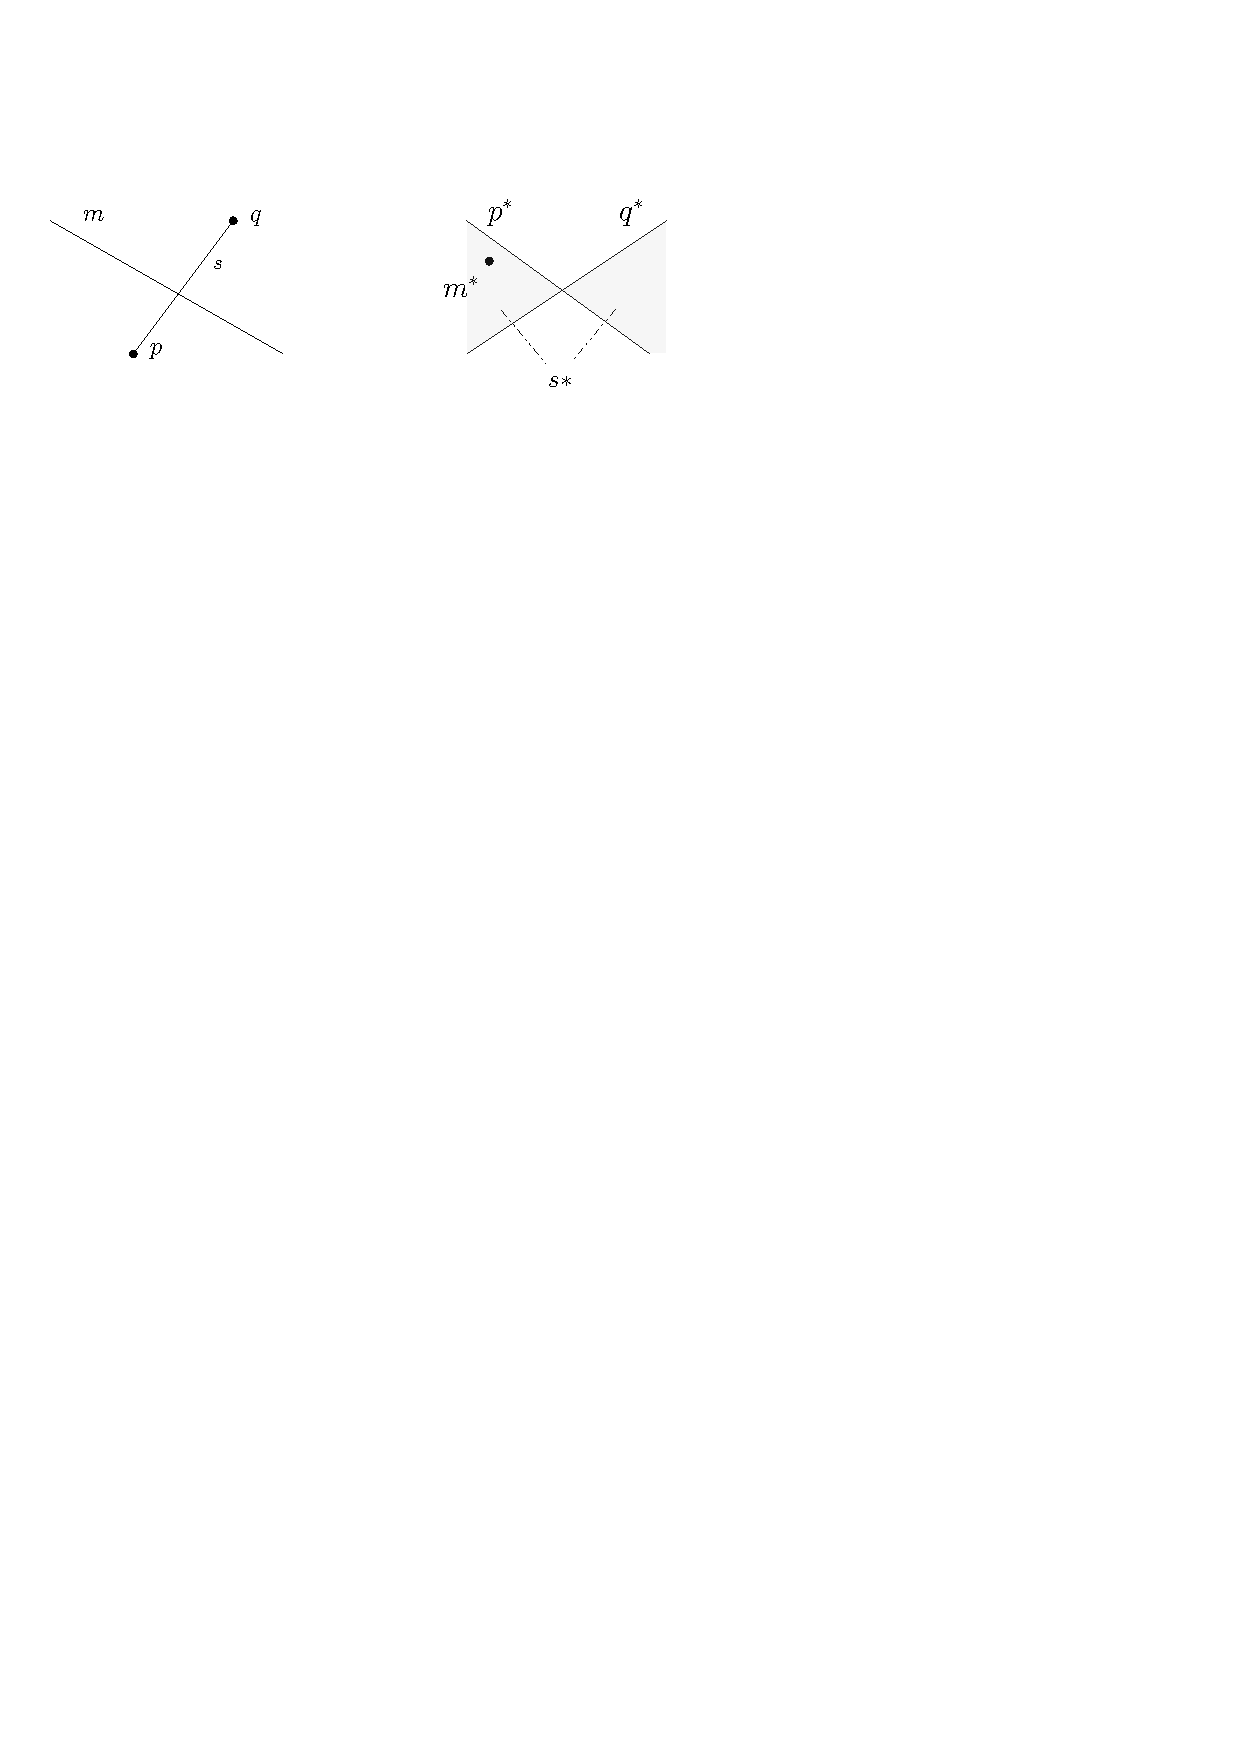
\includegraphics[scale=1]{pics/dual-lines-example.pdf}}
\caption{Na levi sliki sta prikazani točki $p$ in $q$ ter premica $m$ v primarnem prostoru. Desno so v dualnem prostoru prikazani dualni elementi: točka $m*$ ter premici $p*$ in $q*$. S sivo barvo je označeno območje (oziroma del njega), ki jo sestavlja množica točk, ki v primarnem prostoru predstavljajo premice, ki sekajo $s$.} 
\label{dual-ex}
\end{figure}

\subsection{Hitrejši algoritem}
\label{compact}
\begin{figure}
\centerline{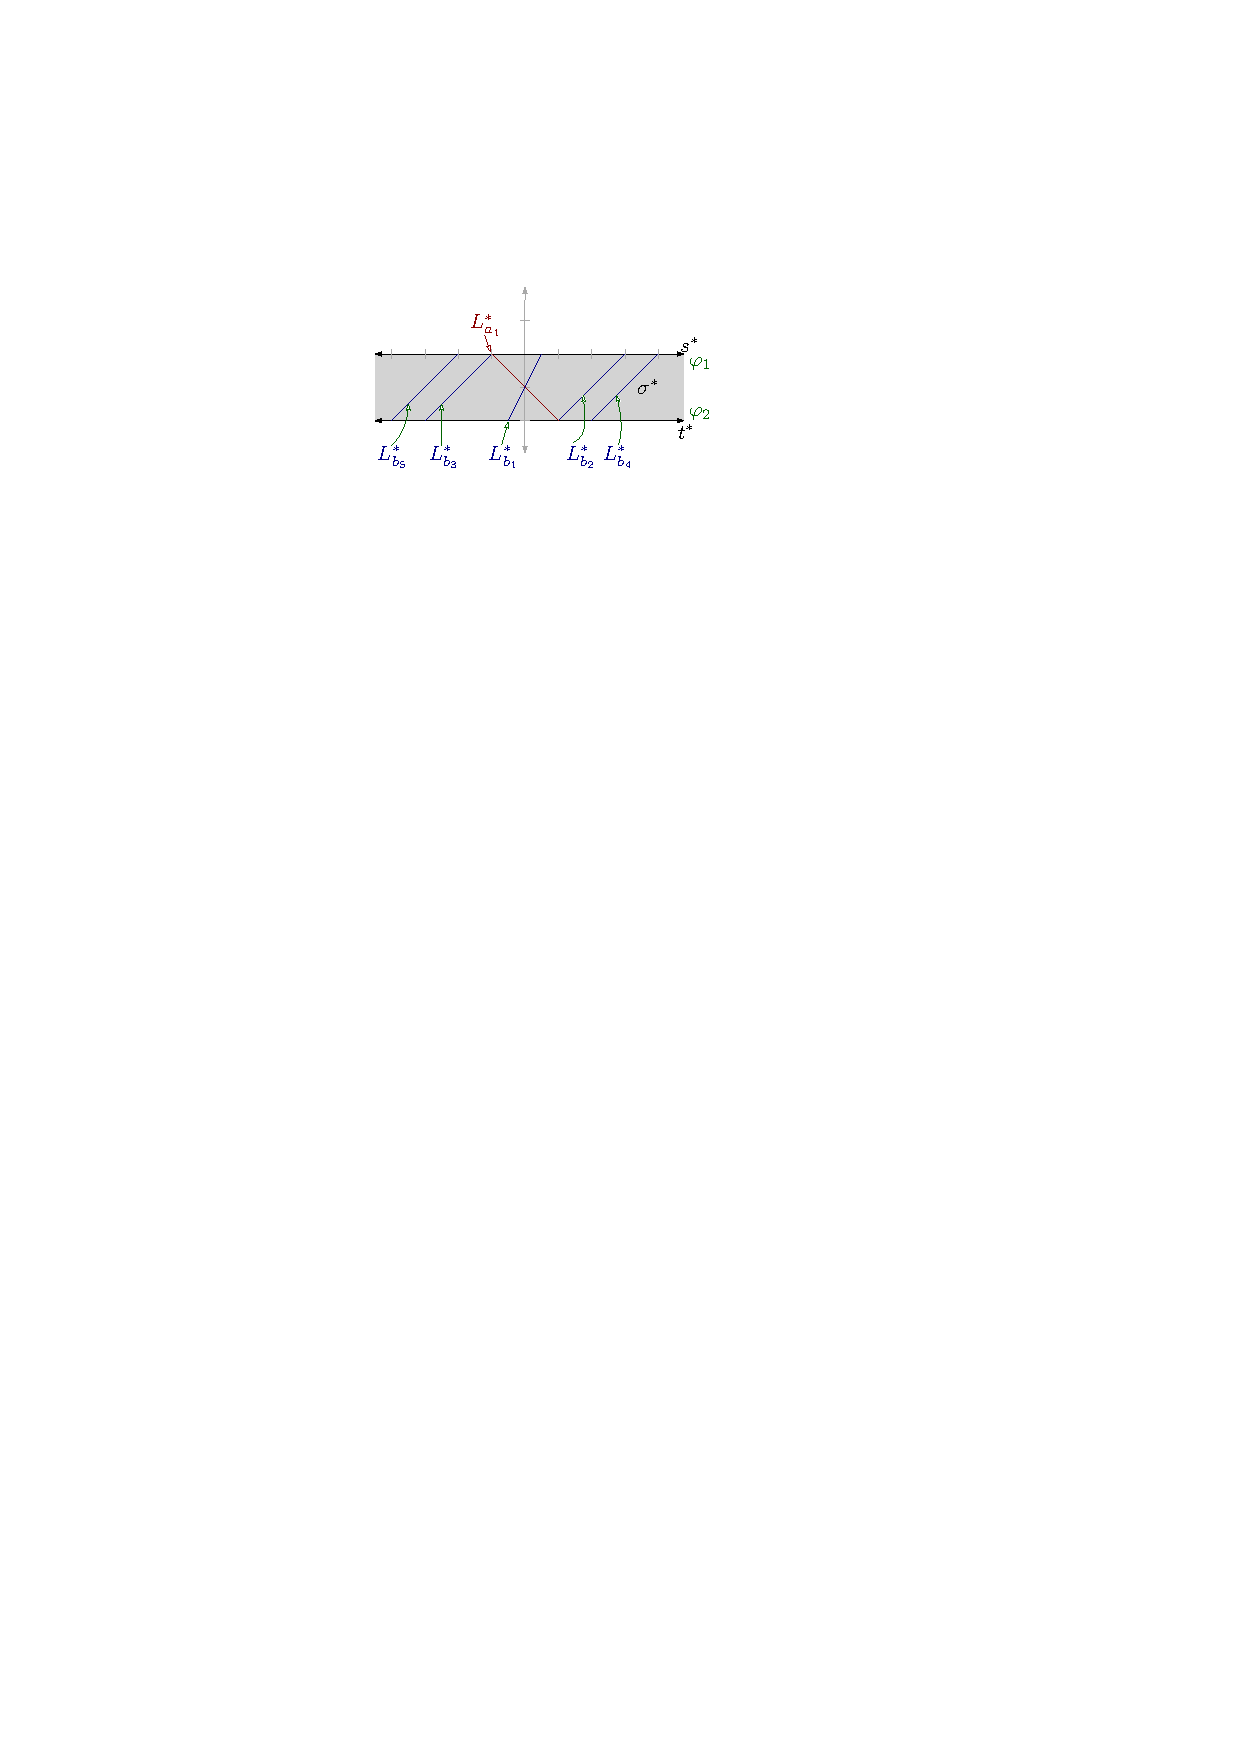
\includegraphics[scale=1]{pics/duality-vertical-slab.pdf}}
\caption{Točke v primarnem prostoru (zgornja slika), njim dualne premice (srednja slika) in slike točk, definirane s preslikavo $\varphi$. Problem iskanja premic $ab_i$, ki sekajo $st$, smo s pomočjo dualnosti preslikali v problem območnega iskanja.} 
\label{hslab}
\end{figure}

\begin{figure}
\centerline{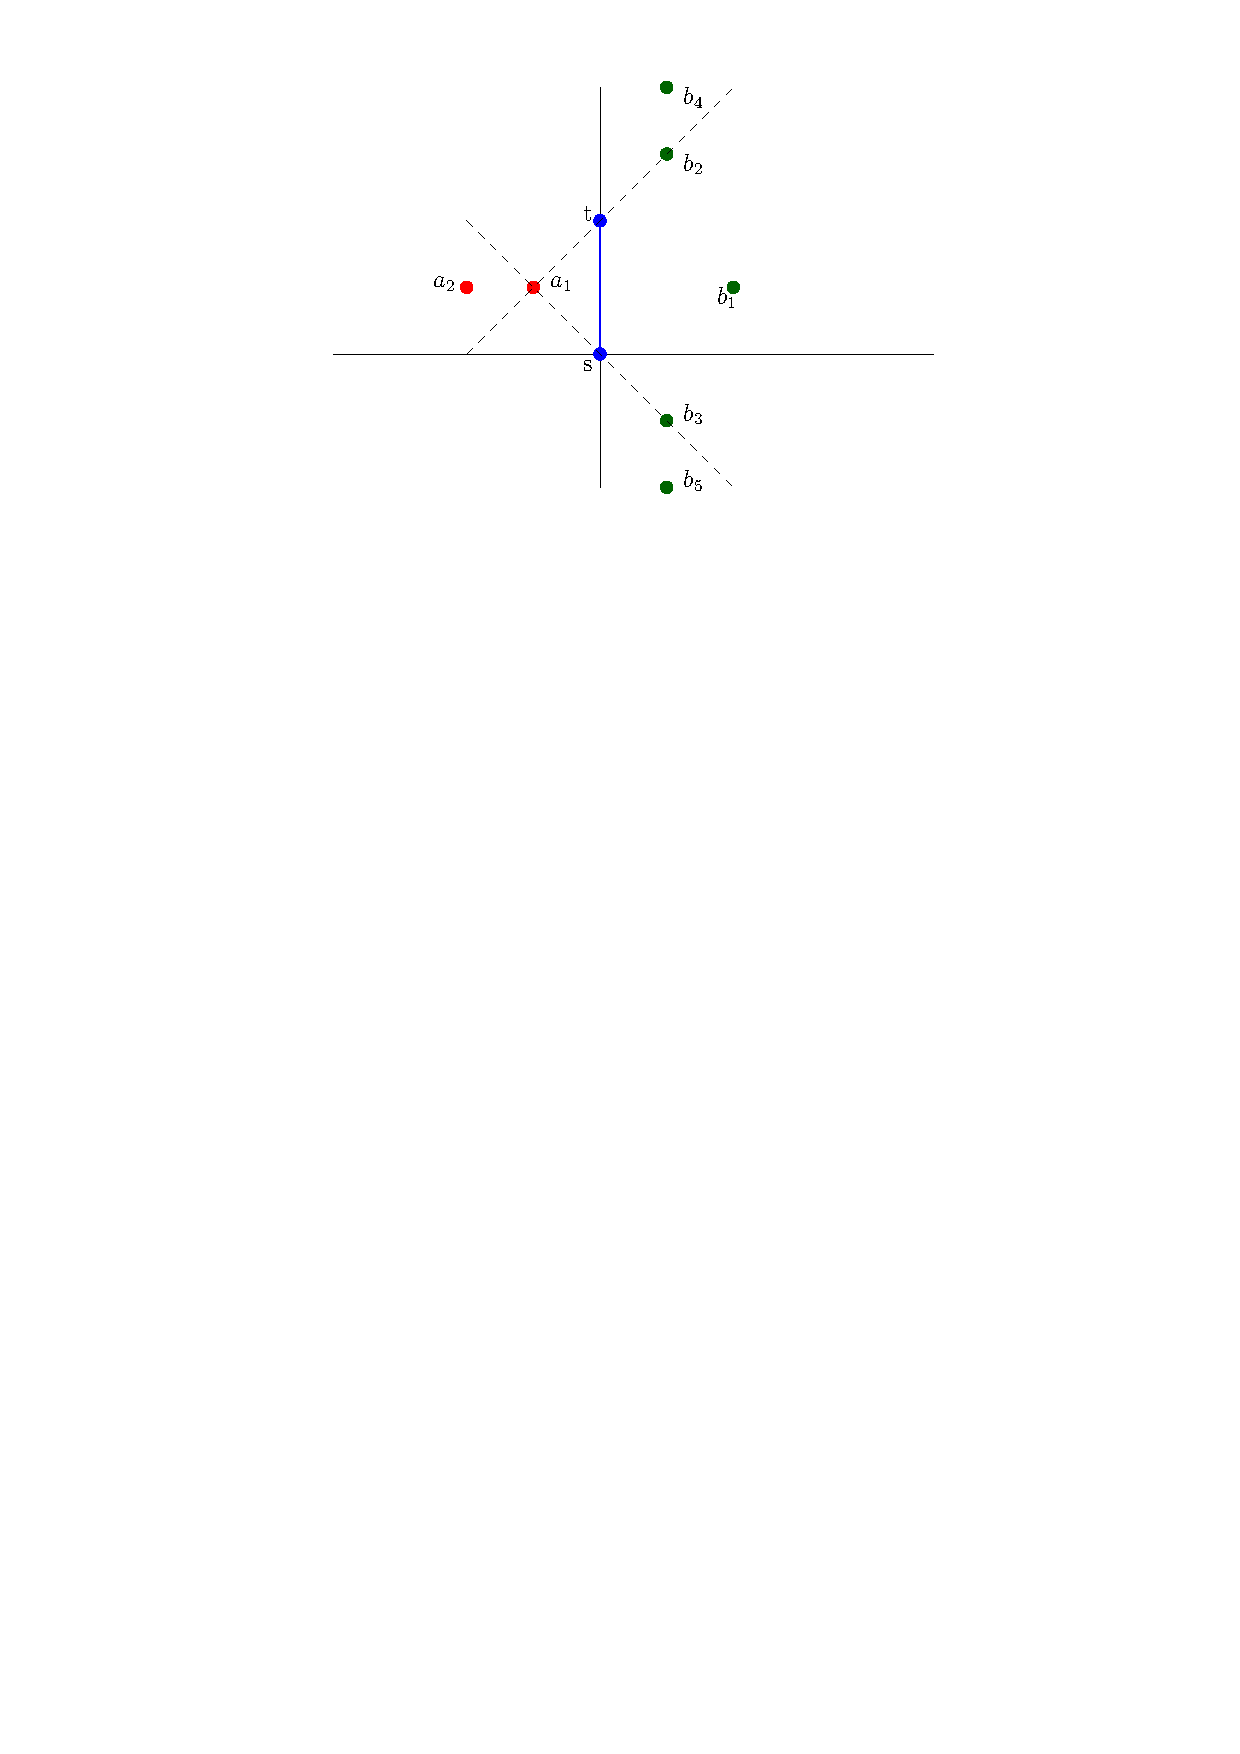
\includegraphics[scale=1]{pics/dual_problem3.pdf}}
\caption{Množici $A$ (rdeči točki) ter $B$ (zelene točke) levo in desno od daljice $st$ (zgornja slika). Črtkani črti predstavljata premici, čigar koeficienta sta uporabljena za izračun koordinat točke preslikave $\varphi (a_1)$, in označujeta vidno polje točke $a_1$.} 
\label{dualp}
\end{figure}

\begin{figure}
\centerline{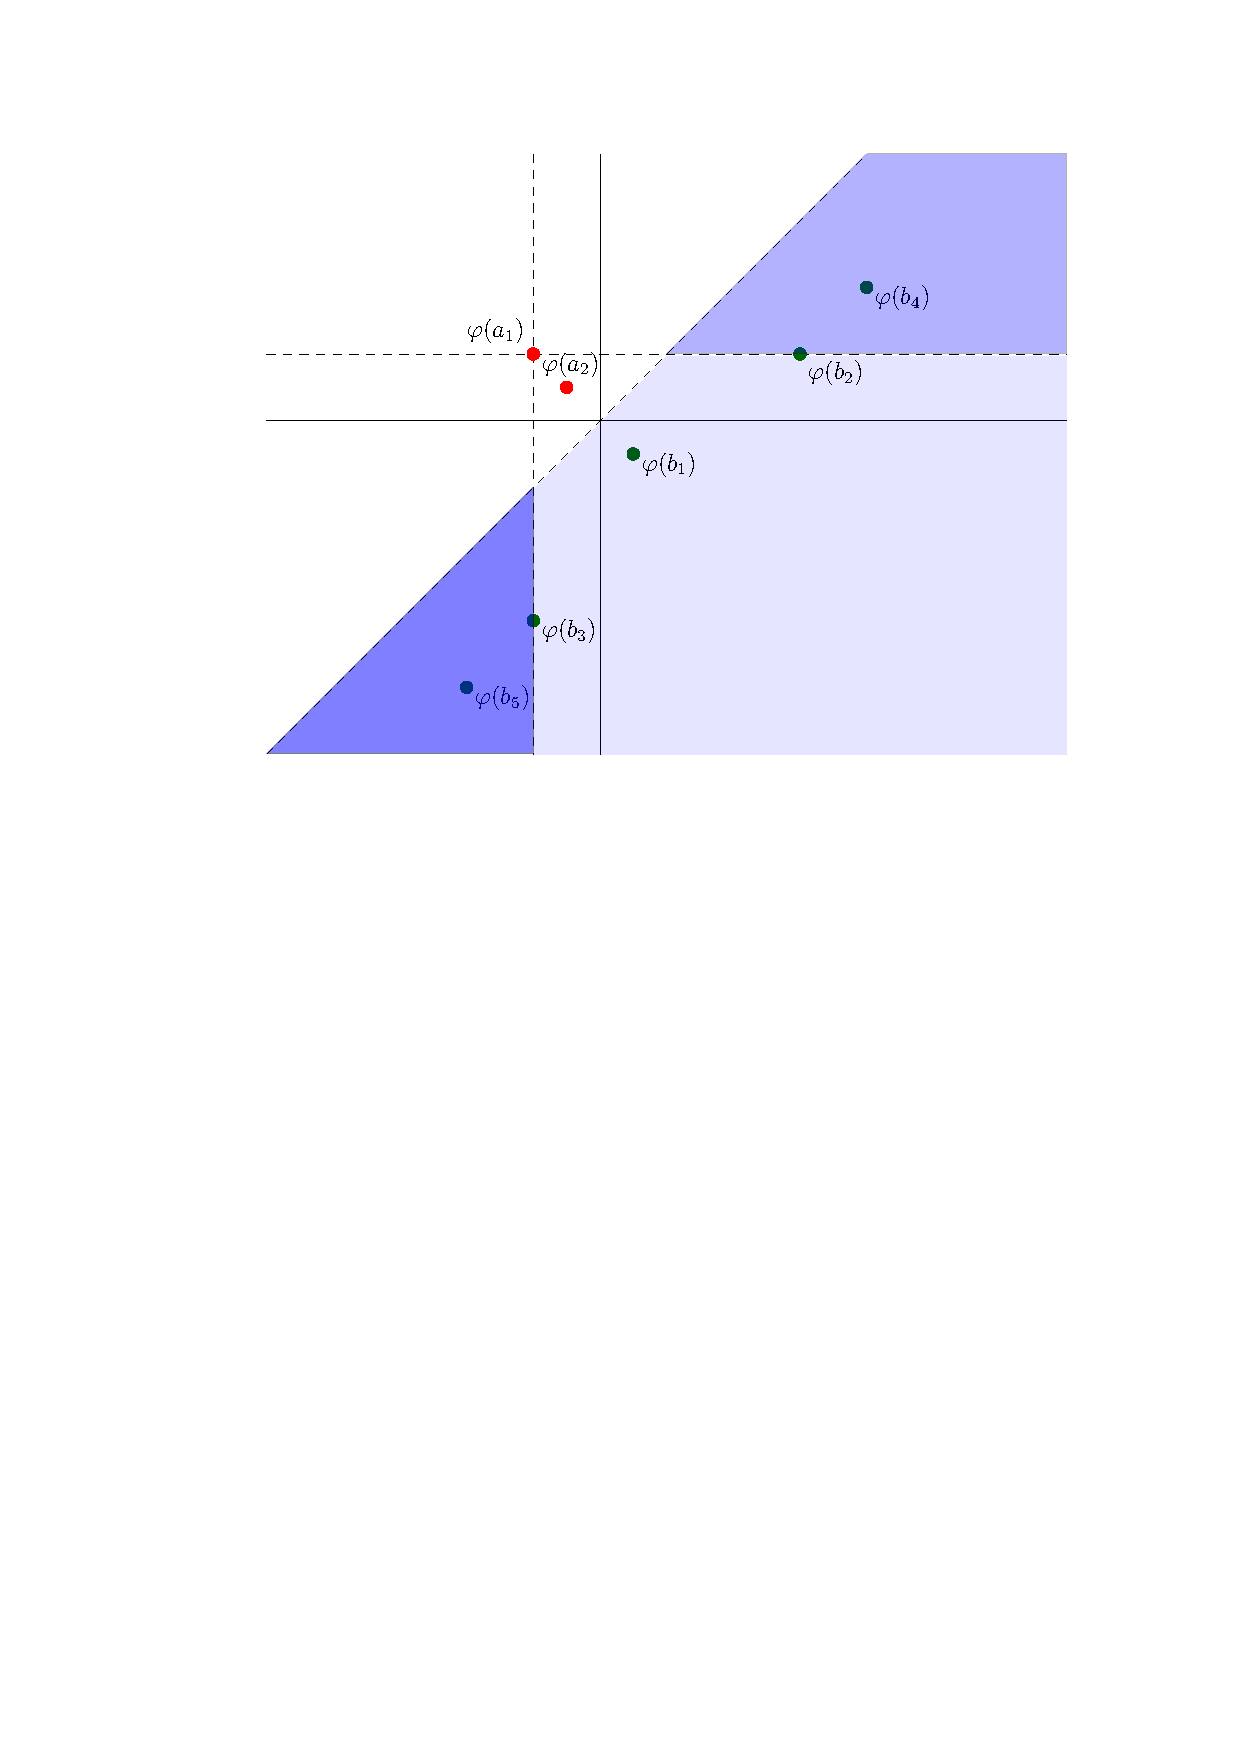
\includegraphics[scale=1]{pics/dual_problem4.pdf}}
\caption{Na sliki so prikazane točke, ki so rezultat preslikave $\varphi$ premic, dualnih točkam na sliki~\ref{dualp}. Obarvano območje v sredini predstavlja prostor, v katerem se nahajajo vse take slike $\varphi (b)$, za katere velja $b \in B(a_1)$. Obarvani območji levo in zgoraj predstavljata prostor slik $\varphi (b)$, za katere velja, da je presečišče premice $a_1b$ z osjo $y$ pod oziroma nad daljico $st$.} 
\label{dualp2}
\end{figure}

Uporabili bomo podatkovno strukturo v naslednji lemi. V osnovi gre za večnivojsko podatkovno strukturo, ki vsebuje dvodimenzionalno območno drevo $T$, slednje pa na vsakem vozlišču sekundarnega drevesa hrani podatkovno strukturo za iskanje najbližjega soseda. 

\begin{lema}
\label{lema-ds2}
Naj bo $A$ množica točk z negativnimi, $B$ pa množica točk z nenegativnimi koordinatami $x$. $B$ lahko predprocesiramo v času $\OO(n\log^3n)$, tako da lahko za vsako točko $a\in A$ v času $\OO(\log^3n)$ določimo, če je množica $\{ b\in B \mid \text{$ab$ seka $\sigma$ in $\|a-b\|\le 1$}\}$ prazna. Z isto podatkovno strukturo lahko obravnavamo poizvedbe za ugotavljanje, ali je množica $\{ b\in B \mid \text{$ab$ ne seka $\sigma$ in }$ \\ $\text{$\|a-b\|\le 1$}\}$ prazna.
\end{lema}

\begin{proof}
Za potrebe dokaza uporabimo dualnost, opisano v prejšnjem poglavju, in območna drevesa.

Naj bo $\LL$ množica nenavpičnih premic, $\sigma^*$ pa množica točk dualnih nevertikalnim daljicam, ki sekajo daljico $\sigma$:

\[
		\sigma^* ~=~ \{ l^* \mid \ell\in \LL, \ell\cap \sigma\neq \emptyset\} 
\]

V dualnem prostoru je množica $\sigma^*$ območje, omejeno z dvema vzporednima premicama
\[
		\sigma^* ~=~ \{ (m,-c)\in \RR^2\mid 0\le c\le \tau\},
\]
ker velja predpostavka $s=(0,0)$ in $t=(0,\tau)$, kjer $\tau\ge 0$.


Za vsako točko $b\in B$ naj bo $L^* _b$ množica točk, dualnih premicam, ki gredo skozi $b$ in sekajo $\sigma$:

\[
		L^*_b=\{ \ell^* \mid \ell\in \LL, b \in \ell, \text{ in } \sigma\cap \ell\not= \emptyset\}.
	\]

Podobno za vsak $a\in A$ definiramo množico točk $L^* _a$. V dualnem prostoru je $L^* _b$ daljica, ki je popolnoma vsebovana v $\sigma^*$ in ima krajišči $(\varphi_1(b),0)$ in $(\varphi_2(b),-\tau)$ na obeh njegovih mejah. Tukaj $\varphi_1(b)$ predstavlja smerni koeficient premice, ki seka točki $s$ in $b$, $\varphi_2(b)$ pa smerni koeficient premice, ki seka točki $t$ in $b$.

Definirajmo točko preslikave $\varphi(b)=(\varphi_1(b),\varphi_2(b))$. Funkcija preslikave $\varphi$ torej preslika točke z nenegativnimi koordinatami $x$ v točke v ravnini.

Za vsak $b\in B$ velja neenakost $\varphi_1(b) \geq \varphi_2(b)$. Točke $B$ lahko razdelimo v tri skupine glede na predznaka koordinat točke preslikave $\varphi(b)$ in za vsako skupino je neenakost očitna:

\begin{align*}
    b_1 \in \{ (x,y) \mid (x,y) \in B, y < 0 \} \Rightarrow &~ \varphi_1(b),\varphi_2(b) < 0 \text{ in } \varphi_1(b) > \varphi_2(b) \\
b_2 \in \{ (x,y) \mid (x,y) \in B, 0 \le y < \tau \} \Rightarrow &~ \varphi_1(b) > 0, \text{ } \varphi_2(b) < 0 \\
    b_3 \in \{ (x,y) \mid (x,y) \in B, y \ge \tau \} \Rightarrow &~ \varphi_1(b) > 0, \text{ } \varphi_2(b) \ge 0 \text{ in }\\ 
    &~\varphi_1(b) > \varphi_2(b)
\end{align*}

Enakost velja le v primeru, ko sta premici, ki definirata obe koordinati, isti. Do slednjega pride pri točkah $b$ s koordinato $x$ enako $0$. 

Iz zgornje neenakosti sledi, da točke preslikave $\varphi(b)$ vedno ležijo na polravnini $x \geq y$ in da je smerni koeficient premice, na kateri leži daljica $L^*_b$, nepozitiven. Podobno lahko ugotovimo, da za vsak $a \in A$ točka $\varphi(a)$ leži na polravnini $\varphi_2(a) > \varphi_1(a)$ in da ima premica, na kateri leži daljica $L^*_a$, pozitiven smerni koeficient.

Naj bo $a \in A$ in $b \in B$. Daljica $ab$ seka daljico $\sigma$ natanko takrat, ko $L^*_a$ seka $L^*_b$, ker daljico $ab$ v dualnem prostoru predstavlja ravno presečišče $L^*_a$ in $L^*_b$. Iz tega sledi naslednja lastnost:

	\[
		ab \cap \sigma \neq \emptyset ~\Longleftrightarrow ~ 
		\varphi_1(a)\le \varphi_1(b) \text{ in } \varphi_2(a)\ge \varphi_2(b).
	\]	
	
Z drugimi besedami: za točko $a \in A$ je množica točk $b \in B$, kjer $ab$ seka $\sigma$, sestavljena iz točk $b$, pri katerih se $\varphi(b)$ nahaja v drugem kvadrantu koordinatnega sistema z izhodiščem $\varphi(a)$. Bolj natančno, gre za točke $\varphi(b)$, ki se nahajajo v preseku drugega kvadranta omenjenega koordinatnega sistema s polravnino $x \geq y$. Glej sliko~\ref{dualp2}.

Za shranjevanje množice točk $\varphi(B)$, kjer se vsaka točka $b \in B$ navezuje na točko preslikave $\varphi(b)$, lahko uporabimo dvodimenzionalno območno drevo. Na vsakem vozlišču $v$ sekundarnega drevesa shranimo podatkovno strukturo za poizvedbe najbližjega soseda nad kanonično množico $P(v)$, ki vsebuje točke shranjene pod $v$ v sekundarnem drevesu. 

Za vsako točko poizvedbe $a \in A$ lahko točke $b \in B$, kjer $ab$ seka $\sigma$, dobimo s poizvedbo na območnem drevesu, ki vrne točke $\varphi(B)$ v kvadrantu

\[
		\{(x,y)\mid  \varphi_1(a) \leq x \text{ in } \varphi_2(a) \geq y\}.
	\]

To pomeni, da množico $\{ b\in B \mid \text{$ab$ seka $\sigma$}\}$ dobimo kot unijo kanoničnih podmnožic $P(v_1),...,P(v_k)$ za $k = \OO(\log^2n)$ vozlišč v sekundarnem drevesu. Za vsako tako podmnožico $P(v_i)$ naredimo poizvedbo najbližjega soseda za točko $a$. Če za nek $v_i$ najdemo najbližjega soseda, ki je za razdaljo največ $1$ oddaljen od $a$, potem vemo, da je množica $\{ b\in B \mid \text{$ab$ seka $\sigma$ in $|ab|\le 1$}\}$ neprazna. V nasprotnem primeru je množica prazna.

Čas zgraditve dvodimenzionalnega območnega drevesa je $\OO(n\log n)$. Vsaka točka se pojavi v $\OO(\log^2n)$ kanoničnih podmnožicah $P(v)$. To pomeni, da $\sum_v |P(v)| = O( n\log^2 n)$, kjer seštejemo $|P(v)|$ za vsa vozlišča $v$ v sekundarnem drevesu. Podatkovno strukturo za iskanje najbližjega soseda lahko v splošnem zgradimo v času $\OO(n\log n)$. Za vsak $v$ jo lahko potem zgradimo v času $O(|P(v)| \log |P(v)|)$. Skupna časovna zahtevnost zgraditve podatkovne strukture je zato $\OO(n\log^3n)$.

Za poizvedbe dvodimenzionalno območno drevo vzame $\OO(\log^2n)$ časa, da  najde $\OO(\log^2n)$ vozlišč $v_1,...,v_k$, tako da velja
\[
		\bigcup_{i=1}^k P(v_i) ~=~ \{ b\in B \mid \text{$ab$ seka $\sigma$}\},
\]
potem pa dodatno potrebujemo $\OO(\log n)$ časa za vsako vozlišče, da naredimo poizvedbo najbližjega soseda. Poizvedbe za $\{ b\in B \mid \text{$ab$ ne seka $\sigma$ in $|ab|\le 1$}\}$ naredimo z isto podatkovno strukturo nad točkami v drugih dveh kvadrantih (glej sliko~\ref{dualp2}).
\end{proof}

Podatkovna struktura za poizvedbe najbližjega soseda v lemi~\ref{lema-ds2} ima časovno zahtevnost zgraditve $\OO(n\log n)$ in časovno zahtevnost poizvedbe $\OO(\log n)$. Če bi uporabili neko drugo podatkovno strukturo za poizvedbe najbližjega soseda s časom zgraditve $T_z(n)$ in časom poizvedbe $T_p(n)$, bi čas zgraditve v lemi~\ref{lema-ds2} postal $O(T_z(n\log^2 n))$, čas poizvedbe pa $O(T_p(n)\cdot \log^2 n)$.

Iz teoretičnega vidika bi bilo bolj učinkovito izračunati unijo
\[
	\bigcup_{b\in B} \{ (x,y)\in \RR^2\mid x<0,~ |(x,y)b|\le 1,~ (x,y) 
			\text{ seka } \sigma \}
\]
in tam rešiti problem določanja položaja (ang. \textit{point location}). Ker območja ne morejo imeti veliko presečišč z daljico $\sigma$, lahko dobimo dobre asimptotične meje. V praksi pa se izkaže, da je izboljšava rezultata zanemarljiva.
\bigbreak
Obravnavajmo zdaj fiksni koren $r$. Predpostavimo, da so drevo najkrajših poti $T_r$ ter tabele $\pi[~]$, $\dist[~]$ in $N[~]$ že izračunane. Točke združimo glede na njihovo razdaljo od $r$:
\[
	W_i ~=~ \{ p\in P \mid \dist[p]=i \},~~~ i=0,1,\dots
\]

Standardna lastnost dreves najkrajših poti je, da se razdalji dveh sosednih točk od korena $r$ razlikujeta za največ $1$. To pomeni, da so sosedi točke $p\in P$ v $G$ vsebovani v $W_{\dist[p]-1}\cup W_{\dist[p]} \cup W_{\dist[p]+1}$. To lastnost bomo uporabili pri našem algoritmu.

Naredimo skupine $L_i^j$ in $D_i^j$, kjer $L$ pomeni ``levo", $D$ pomeni ``desno" ter $j=0,1$ in $i=0,1,...$, definirane kot
\begin{align*}
	L_i^j ~&=~ \{ p\in P \mid \dist[p]=i,~ p.x<0,~ N[p]=j \} \\
	D_i^j ~&=~ \{ p\in P \mid \dist[p]=i,~ p.x>0,~ N[p]=j \}
\end{align*}
Zanimajo nas povezave $pq$ v $G$, za katere velja $N[p]+N[q]+\CR(st,pq)=1 \pmod 2$. Z upoštevanjem simetrije je to ekvivalentno parom točk $(p, q)$ v enem od naslednjih dveh primerov:
\begin{itemize}
	\item za nek $i\in \NN$ in nek $j\in \{0,1\}$ imamo
			$p\in L_i^j\cup R_i^j$, 
			$q\in L_i^{1-j}\cup R_i^{1-j}\cup L_{i-1}^{1-j}\cup R_{i-1}^{1-j}$, 
			$\|p-q\|\le 1$, in $pq$ ne seka $st$;
	\item za nek $i\in \NN$ in nek $j\in \{0,1\}$ imamo
			$p\in L_i^j\cup R_i^j$, 
			$q\in L_i^{j}\cup R_i^{j}\cup L_{i-1}^{j}\cup R_{i-1}^{j}$, 
			$\|p-q\|\le 1$, in $pq$ seka $st$.
\end{itemize}
Oba primera se da učinkovito rešiti z enim od naslednjih primerov:
\begin{itemize}
\item Če želimo iskati kandidate $(p,q)\in L_i^j\times L_{i'}^{1-j}$ (ki ne morejo sekati $st$, ker ležijo na isti strani osi $y$), najprej preprocesiramo $L_{i'}^{1-j}$ za poizvedbe najbližjega soseda. Potem za za vsako točko $p$ v $L_i^j$ naredimo poizvedbo nad podatkovno strukturo, da najdemo njenega najbližjega soseda $q_p$ v $L_i^j$. Če za nek $p$ velja $|pq_p|\le 1$, smo našli povezavo $pq_p$ v $G$, za katero velja $\CR(\cycle(T_r,pq_p))=1$ in $\dist[p]+\dist[q_p]+1=i+i'+1$. Če za vsak $p$ velja $|pq_p|> 1$, potem $L_i^j\times L_{i'}^{1-j}$ ne vsebuje nobene povezave iz $G$. Če $m=|L_i^j|+|L_{i'}^{1-j}|$, je skupni čas izvajanja $\OO(m\log m)$.
\item Če želimo iskati kandidate $(p,q)\in L_i^j\times R_{i'}^{j}$, ki sekajo $st$, najprej preprocesiramo $R_{i'}^{j}$ v podatkovno strukturo, kot smo opisali v lemi~\ref{lema-ds2}. Nato za vsako točko $p\in L_i^j$ naredimo poizvedbo na podatkovni strukturi za take točke $q$, da $pq$ seka $st$. Če kot rezultat dobimo neprazno množico, potem obstaja $pq$ v $G$, za katero velja $p\in L_i^j$, $q\in R_{i'}^{j}$, $\CR(\cycle(T_r,pq))=1$ in $\dist[p]+\dist[q]+1=i+i'+1$. V nasprotnem primeru ne obstaja nobena povezava $pq\in L_i^j\times R_{i'}^{j}$, ki bi sekala $st$. Za $m=|L_i^j|+|R_{i'}^{j}|$ je skupni čas izvajanja  $O(m\log^3 m)$.
\item Če želimo iskati kandidate $(p,q)\in L_i^j\times R_{i'}^{1-j}$, ki ne sekajo $st$, najprej preprocesiramo $R_{i'}^{1-j}$ v podatkovno strukturo, kot smo opisali v lemi~\ref{lema-ds2}. Nato za vsako točko $p\in L_i^j$ naredimo poizvedbo na podatkovni strukturi za take točke $q$, da $pq$ ne seka $st$. Preostali potek algoritma je podoben kot v prejšnji točki. 
\end{itemize}
Sklenemo lahko, da vsakega od primerov lahko rešimo v času $\OO(m\log^3m)$ v najslabšem primeru, kjer je $m$ število točk udeleženih v posameznem primeru. Z iteracijo čez vse možne vrednosti $i$ je zdaj to preprosto pretvoriti v algoritem, ki porabi $\OO(n\log^3n)$ časa za vsak koren $r$. Za primer z enotskimi krogi ta algoritem izboljša čas splošnega algoritma. 
\begin{izrek}
\label{lema4}
Problem minimalne ločitve $n$ enotskih krogov lahko rešimo v času $\OO(n^2\log^3n)$.
\end{izrek}

\begin{proof}
Naj bodo $P$ središča krogov in - tako kot prej - obravnavajmo graf $G=\GG(P)$. Za vsak $r\in P$ zgradimo drevo najkrajših poti in množice $W_i,L_i^0,L_i^1,R_i^0,L_i^1$ za vsak $i$ v času $O(n\log n)$. Nato imamo največ $n$ iteracij, kjer za vsako iteracijo $i$ porabimo $O(|W_i\cup W_{i-1}|\log^3 |W_i\cup W_{i-1}|)$ časa. Množice $w_i$ so disjunktne in če seštejemo čase vseh iteracij, je čas izvajanja za posamezen koren $r\in P$ enak $\OO(n\log^3n)$.

Pravilnost algoritma sledi iz dejstva, da računa isto kot splošni algoritem.
\end{proof}

%\begin{figure}[htb]
%\begin{center}
%\ovalbox{~~~~
%\begin{varwidth}{\linewidth}
%\begin{codebox}
%    \Procname{// Delo za koren $r\in P$}
%   	\li $(\dist[~],\pi[~])\gets$ drevo najkrajših poti iz $r$ v $\GG(P)$
%	\li Izračunaj nivoje $W_0,W_1,\dots$
%	\li \For $i=0\dots n$ \Do
%		\li Izračunaj $N[p]$ za vsak $p$ v $W_i$
%		\li Izračunaj $L^0_i$, $L^1_i$, $R^0_i$, $R^1_i$
%		\End
%    \li $i=1$
%    \li \While $2i< \best$ in $W_i\neq\emptyset$ \Do
%		\\ \> // znotraj obeh strani osi $y$ 
%		\li išči kandidate v \\
%			\> ~~~$L^0_i\times L^1_{i-1}$, $L^1_i\times L^0_{i-1}$, 
%				$R^0_i\times R^1_{i-1}$, \\
%			\> ~~~$R^1_i\times R^0_{i-1}$,
%				$L^0_i\times L^1_{i}$ in $R^0_i\times R^1_{i}$
%		\\ \> // preko osi $y$ skozi $\sigma$
%		\li išči kandidate, ki sekajo $\sigma$ v \\
%			\> ~~~$L^0_i\times R^0_{i-1}$, $L^1_i\times R^1_{i-1}$, 
%				$L^0_{i-1}\times R^0_{i}$, \\
%			\> ~~~$L^1_{i-1}\times R^1_{i}$, $L^0_i\times R^0_{i}$ 
%				in $L^1_i\times R^1_{i}$
%		\\ \> // preko osi $y$ mimo $\sigma$			
%		\li išči kandidate, ki ne sekajo $\sigma$ v \\
%			\> ~~~$L^0_i\times R^1_{i-1}$, $L^1_i\times R^0_{i-1}$, 
%				$L^1_{i-1}\times R^0_{i}$, \\ 
%			\> ~~~$L^0_{i-1}\times R^1_{i}$, $L^0_i\times R^1_{i}$ 
%				in $L^1_i\times R^0_{i}$		
%		\li $i \gets i+1$
%		\End
%    \\[-2mm]
%\end{codebox}
%\end{varwidth}
%~~~~}\end{center}
%\caption{Work for each vertex in the new algorithm for minimum separation with unit disks.}
%\label{fig:compact}
%\end{figure}

\begin{figure}[htb]
\begin{center}
\scalebox{.92}{%
\ovalbox{~~~~
\begin{varwidth}{\linewidth}
\begin{codebox}
    \Procname{$\proc{SeparationUnitDisksCompact}(P,s,t)$}
    \li $\best \gets n+1$ // dolžina trenutno najboljše ločitve
    \li \For $r\in P$ \Do
    	\li $(\dist[~],\pi[~])\gets$ drevo najkrajših poti s korenom $r$ v $\GG(P)$
		\\ \> // Izračunaj nivoje $W_i$
    	\li \For $i=0\dots n$ \Do
			\li $W_i\gets$ nov prazen seznam
			\End
    	\li \For $p\in P$ \Do
			\li dodaj $p$ v $W_{\dist[p]}$
			\End		
		\\ \> // Izračunaj $N[~]$ za vse elemente v $W_i$
		\\ \> // in zgradi $L_i^0,L_i^1,R_i^0,R_i^1$
    	\li $N[r]=0$
		\li \For $i=1\dots n$ \Do
			\li \For $p\in W_i$ \Do
				\li $N[p]= N[\pi[p]]+ \CR(st,p\pi[p]) \pmod 2$
				\li \If $p$ levo od $y$ osi \Then
					\li dodaj $p$ v $L^{N[p]}_i$
					\End
				\li \If $p$ desno od $y$ osi \Then
					\li dodaj $p$ v $R^{N[p]}_i$
					\End
				\End
			\End
    	
\end{codebox}
\end{varwidth}~~~~}}
\end{center}
\caption{Nov algoritem za minimalno ločitev z enotskimi krogi (prvi del).}
\label{fig:FULL}
\end{figure}

\begin{figure}[htb]
\begin{center}
\scalebox{.92}{%
\ovalbox{~~~~
\begin{varwidth}{\linewidth}
\begin{codebox}
		\li \Do $i=1$
    	\li \While $2i< \best$ in $W_i\neq \emptyset$ \Do
			\\ \>\> // dolžina $2i$; znotraj vsake strani $y$ osi 
			\li išči kandidate v $L^0_i\times L^1_{i-1}$, $L^1_i\times L^0_{i-1}$,
			$R^0_i\times R^1_{i-1}$, $R^1_i\times R^0_{i-1}$
			\\ \>\> // dolžina $2i$; čez $y$ os skozi $\sigma$
			\li išči kandidate, ki sekajo $\sigma$ v 
			\li $L^0_i\times R^0_{i-1}$, $L^1_i\times R^1_{i-1}$, $L^0_{i-1}\times R^0_{i}$, $L^1_{i-1}\times R^1_{i}$
			\\ \>\> // dolžina $2i$; čez $y$ os mimo $\sigma$			
			\li išči kandidate, ki ne sekajo $\sigma$ v 
			\li $L^0_i\times R^1_{i-1}$ , $L^1_i\times R^0_{i-1}$, $L^0_{i-1}\times R^1_{i}$,$L^1_{i-1}\times R^0_{i}$
			\\ \>\> // dolžina $2i+1$; znotraj vsake strani $y$ osi 
			\li išči kandidate v $L^0_i\times L^1_{i}$, $R^0_i\times R^1_{i}$
			\\ \>\> // dolžina $2i+1$; čez $y$ os skozi $\sigma$
			\li išči kandidate, ki sekajo $\sigma$ v $L^0_i\times R^0_{i}$, $L^1_i\times R^1_{i}$ 
			\\ \>\> // dolžina $2i+1$; čez $y$ os mimo $\sigma$			
			\li išči kandidate, ki ne sekajo $\sigma$ in $L^0_i\times R^1_{i}$, $L^1_i\times R^0_{i}$
			\li $i \gets i+1$
			\End
		\End
    \li \Return $\best$
    \\[-2mm]
\end{codebox}
\end{varwidth}~~~~}}
\end{center}
\caption{Nov algoritem za minimalno ločitev z enotskimi krogi (drugi del).}
\label{fig:FULL2}
\end{figure}

Opis algoritma v obliki psevdokode je prikazan na sliki~\ref{fig:FULL}. Kot pri splošnem algoritmu spremenljivka $best$ hrani dolžino trenutno najkrajšega cikla. Na začetku lahko njeno vrednost nastavimo na $n+1$. Če algoritem konča z isto vrednostjo spremenljivke, potem za dane točke ne obstaja rešitev za problem minimalne ločitve. Ko obravnavamo določen koren $r$, nas zanimajo samo cikli s korenom $r$ in dolžino največ $best$. Ker ima poljuben cikel, ki gre skozi vozlišče v $W_i$, dolžino najmanj $2i$, lahko obravnavamo samo indekse $i$, za katere velja $2i < best$. Poleg tega lahko dodatno omejimo iskanje (kar sicer ni opisano v algoritmu, je pa uporabljeno pri implementaciji) tako, da najprej obravnavamo pare, ki tvorijo cikel z dolžino $2i$, na primer $L^0_i\times L^1_{i-1}$, in šele potem tiste z dolžino $2i+1$, na primer $L^0_i\times L^1_i$. Z uporabo takega zaporedja lahko končamo z iskanjem za koren $r$ takoj, ko najdemo povezavo v $while$ zanki, in preidemo na naslednji koren.

\chapter{Implementacija algoritmov}
\label{ch3}

V nadaljevanju sta opisani implementaciji algoritma za drevo najkrajših poti v grafu enotskih krogov iz~\cite{CJ15}, ki je bil opisan v poglavju~\ref{sssp-tree}, in algoritma za minimalno ločevanje z enotskimi krogi, opisanega v poglavju~\ref{compact}. Gre za razširjen opis implementacije iz~\cite{CM}.

\section{Drevo najkrajših poti v grafu enotskih krogov}

Algoritem SSSP za izgradnjo drevesa najkrajših poti smo implementirali z mislijo na možnost njegove neposredne uporabe v algoritmu za ločevanje s krogi. Posledično smo spustili nekaj funkcionalnosti dreves, ki jih kasneje v programu ne potrebujemo, po drugi strani pa dodali funkcionalnosti, ki se ne tičejo drevesa, so pa potrebne kasneje pri ločevanju. Tako na primer ne moremo dostopati do otrok vozlišč drevesa, po drugi strani pa imamo pri dodajanju točk v drevo slednje možnost shraniti v množice $L_i^j, R_i^j$, itd.

Za implementacijo smo napisali razred $SSSPTree$, ki kot notranje stanje v enem izmed svojih atributov hrani DT. Slednjo zgradi natanko enkrat pri inicializaciji. Konstruktor kot argument sprejme seznam točk $P$, z metodo \textit{createTreeFromRoot(Point\U 2 r)} pa zgradi drevo.

\subsection{Podatkovna struktura za točko}
\label{point-refs}
Algoritem zgradi drevo implicitno. To pomeni, da kot rezultat ne dobimo nobene nove strukture, ampak vsaki točki vozlišča DT spremeni vrednost njenih sledečih atributov:

\begin{description}
\item[dist] hrani razdaljo do korena drevesa. Koren drevesa ima za razdaljo vrednost $0$, točke, ki jih ni moč doseči iz korena, pa največjo možno vrednost števila tipa $int$, tj. \textit{numeric\U limits\textless int \textgreater ::max()}
\item[parent] hrani deljen kazalec (\textit{shared\U ptr\textless Point\U 2 \textgreater}) na svojega starša v drevesu
\item[visited] hrani logično vrednost, ki pove, če je vozlišče bilo že dodano v drevo. To bi sicer lahko izvedeli tudi preko atributa $dist$
\end{description}

Noben izmed omenjenih atributov ni del razreda $Point\U 2$ v CGAL, zato smo jih dodali sami. S pomočjo kazalca na starša se je tako od vsakega vozlišča drevesa možno sprehoditi do korena. Omeniti je treba tudi, da objekti tipa \textit{Point\U 2}, ki so shranjeni v vozliščih DT, niso isti objekti kot tisti, ki so podani v seznamu kot argument konstruktorju, temveč objekt razreda DT v CGAL-u ustvari lastne kopije. Spremembe atributov točk se zato ne odrazijo na podanem vhodnem vektorju točk. 

Preden lahko kakorkoli uporabljamo točke tipa \textit{Point\U 2}, moramo za njih izbrati še način predstavitve in jedro. Odločili smo se uporabiti \textit{Cartesian\textless double \textgreater}. Kartezična predstavitev je bolj intuitivna, poleg tega pa v algoritmu ne uporabljamo nikakršnega deljenja, zaradi katerega bi razmišljali o uporabi homogene predstavitve. Podoben argument velja za uporabo številskega tipa $double$. V algoritmu ne računamo nobenih novih točk, za že dane točke pa predpostavljamo, da imajo natančne koordinate. Poleg tega namesto prave razdalje med točkami računamo kvadrat razdalje, s čimer se izognemo uporabi deljenja (pri enotskih krogih je med drugim priročno tudi dejstvo, da je preverjanje razdalje ekvivalentno preverjanju kvadrata razdalje).

\subsection{Podatkovna struktura za iskanje najbližjega soseda}
\label{why dt}

Kot smo omenili pri teoretičnem opisu algoritma v poglavju~\ref{sssp-tree}, pri gradnji množice $W_i$ testiramo kandidatne točke tako, da poiščemo njihove najbližje sosede v množici $W_{i-1}$. Nad slednjo zgradimo VD, kandidatne točke pa uporabimo za poizvedbe nad tako strukturo.

V praksi se pri uporabi knjižnice CGAL izkaže, da je za iskanje najbližjega soseda bolje uporabiti DT. Do tega sklepa smo prišli z analizo implementacije obeh struktur:

\begin{itemize}
\item Za iskanje najbližjega soseda z VD uporabimo funkcijo $locate(Point$ $q)$, ki za rezultat vrne Voronoijevo celico, rob ali vozlišče. V našem primeru vedno iščemo najbližje Voronoijevo središče, tako da v primeru, da je rezultat vozlišče ali rob, vrnemo enega od enako oddaljenih središč. Ker v CGAL-u objekt VD interno hrani strukturo DT, v praksi potemtakem pravzaprav iščemo vozlišče v DT. Funkcija $locate$ za izračun uporablja funktor za iskanje najbližjega Delaunayevega vozlišča, ki je definiran z drugo predlogo VD-ja. Imenuje se \textit{Delaunay\U triangulation\U nearest\U site\U 2}. Ta nato kliče funkcijo \textit{nearest\U vertex (Point q)} v DT. Rezultat slednje je pravzaprav tisto, kar iščemo od samega začetka, zato se lahko znebimo VD kot vmesnika in direktno uporabljamo DT. 
\item Poleg poenostavitve kode in rešitve je pomemben faktor tudi optimizacija. Problem najbližjega soseda je rešljiv v času $\OO(\log n)$, vendar ne z uporabo DT. Povprečna časovna zahtevnost funkcije \textit{nearest\U vertex(Point q)}, ki za iskanje najbližjega vozlišča uporablja sprehod po povezavah triangulacije (angl. \textit{line walk}), je $\OO(\sqrt{n})$. DT pa v CGAL-u vsebuje tudi funkcijo \textit{nearest\U vertex(Point q, Face\U handle hint)}, kateri kot drugi argument podamo lice v DT, pri katerem se iskanje začne. Če znamo podati dobro začetno lice, se časovna zahtevnost bistveno zmanjša (na $k$ korakov, kjer $k << n$). Problem pri uporabi VD je potem tudi ta, da njena funkcija \textit{locate} ne podpira dodatnega argumenta za začetno lice. Tudi če bi tako funkcijo napisali sami, bi nastal problem pri tem, kako najti primerno lice VD-ja oziroma kako dostopati do njega. 
\item Sama izbira lica v DT je očitna. Za točko $q$, ki jo dobimo iz vrste, in točko $p$, s katero tvorita povezavo v DT(P) (glej psevdokodo~\ref{fig:SSSP}), imamo za poizvedbo točki $p$ najbližjega vozlišča dve možnosti za dobrega kandidata za začetno lice. Če $q\in DT(W_{i-1})$, je smiselen kandidat katerokoli lice vozlišča $q$, sicer pa je to katerokoli lice starša točke $q$ v drevesu SSSP, ker je starš zagotovo vsebovan v $DT(W_{i-1})$. 
\end{itemize}

Za razliko od VD, ki ima samo metodo za vstavljanje ene točke v strukturo, DT vsebuje tudi metodo, ki kot argument sprejme seznam točk. Te nato prostorsko sortira, preden jih eno po eno doda v strukturo~\cite{cgal:dd-ss-15a}. Prednost sortiranja je v tem, da so bili deli strukture, ki so obravnavani med vstavljanjem, z veliko verjetnostjo obravnavani tudi pri prejšnjem vstavljanju, in se zato z večjo verjetnostjo nahajajo v predpomnilniku kot v glavnem pomnilniku. Uporaba sortiranja ni optimalna izbira na vseh primerih vhodnih podatkov. Pri našem algoritmu se je izkazalo, da algoritem deluje počasneje, zato smo metodo prilagodili tako, da točk ne sortira. To niti ni toliko presenetljivo: vhodne točke, ki jih DT v $i$-ti iteraciji dobi iz seznama $W_{i-1}$, so deloma že smiselno sortirane. Poglejmo si, kako je zgrajen seznam $W_1$, ki vsebuje točke z razdaljo 1 od korena $r$. Za iskanje sosedov vozlišča $r$  uporabimo krožni iterator, ki se začne pri poljubnem sosedu in se nato s pomočjo lic premika do naslednjega. Sosedi si zato sledijo v smiselnem zaporedju, v katerem so tudi shranjeni v seznam $W_1$. Ko obiščemo vse sosede, moramo obiskati še vse sosede sosedov. Začnemo pri prvem obiskanem sosedu, in zopet s krožnim iteratorjem pogledamo vse sosede, in tako naprej do ostalih. V splošnem velja, da bodo sosedje soseda $i$ bolj blizu sosedom soseda $i+1$ kot soseda $i+2$, in s prvimi bolj verjetno tvorili povezavo v $DT(W_i)$ kot z drugimi. Drugače povedano: za novonastali trikotnik, ki je dodan v triangulacijo, je velika verjetnost, da meji na trikotnik, dodan v prejšnjem koraku.

\bigbreak

Za učinkovito iskanje začetnega lica smo napisali razširitev razreda za DT v CGAL-u, imenovano \textit{DTWithFaceMap}. Hrani zasebni slovar \textit{pointsToFaceHandlers}, ki kot ključ hrani kazalec na objekt tipa \textit{Point\U 2}, kot vrednost pa objekt tipa \textit{DT\U Face\U handle}. Vsebuje tudi dodatno metodo za vstavljanje, ki kot argument sprejme seznam vozlišč tipa \textit{DT\U vertex\U handle}. Iz vsakega objekta vozlišča dobi ven točko tipa \textit{Point\U 2}, ki jo vstavi v DT z metodo \textit{insert(Point\U 2 q)}, ki je že definirana  v razredu DT. Ta metoda vrne nov objekt vozlišča, ki je bilo dodano v strukturo. Objekt hrani informacijo o točki $q$ in licu $f$, na katerega vozlišče meji. Par \textit{(q, f)} nato shranimo v slovar \textit{pointsToFaceHandlers}.

Pomembno dejstvo, ki ga je potrebno izpostaviti, je sledeče. Teoretično gledano je množica točk v DT($W_i$) podmnožica točk v DT(P). Ker CGAL razlikuje med vozlišči in točkami, triangulaciji za vozlišče $v$, ki ga obe vsebujeta, hranita vsak svoj lasten objekt. Oba objekta vozlišča pa hranita referenco na isto instanco točke, saj \textit{DTWithFaceMap} za razliko od DT ne sortira točk.


Koda, ki se izvede za posamezno vozlišče $p$, je sledeča:

\begin{quote}
f = DT::insert((*p)-$>$point(), f)-$>$ face();\\
pointsToFaceHandlers[\&((*p)-$>$point())] = f;
\end{quote}

%\begin{figure}
%\centerline{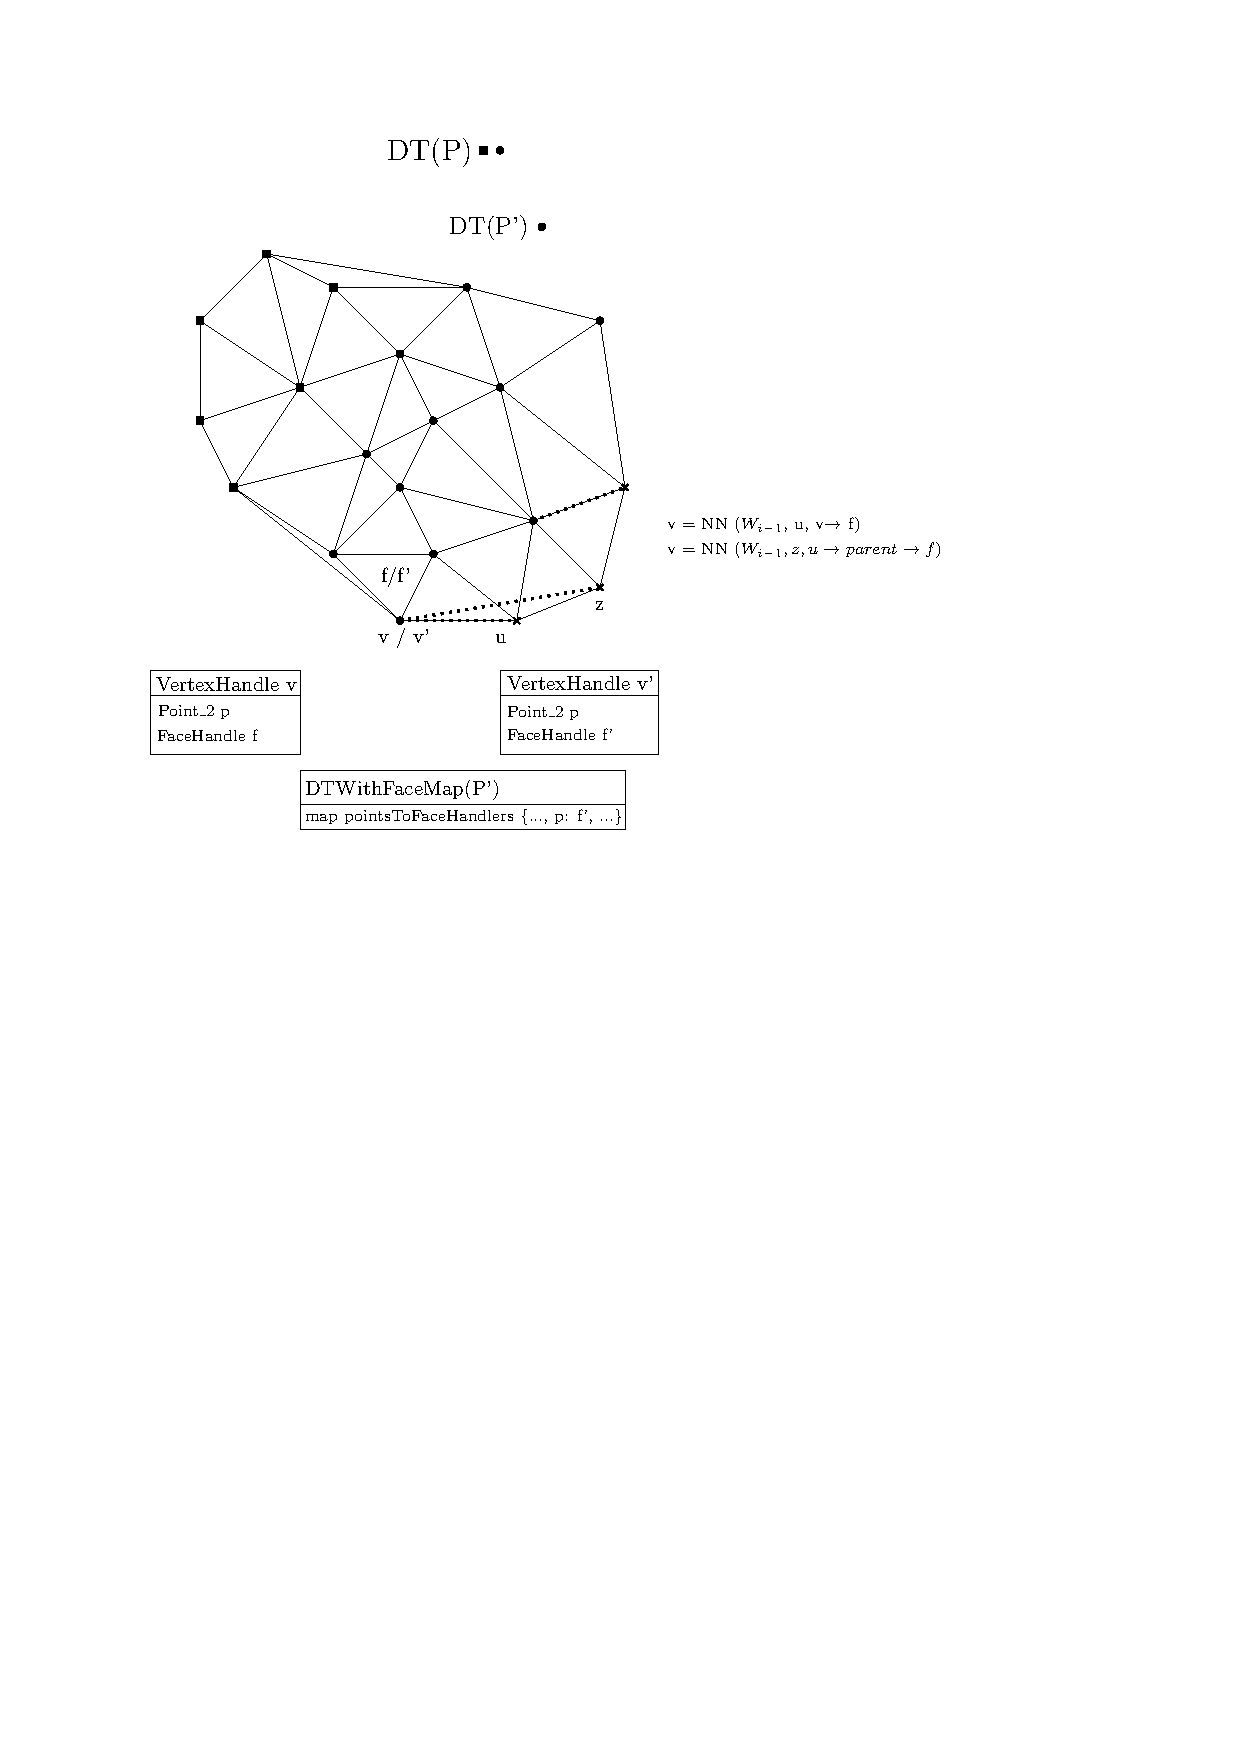
\includegraphics{pics/pointsToFaceHandlers.pdf}}
%\caption{.}
%\label{pointsToFace}
%\end{figure}
\subsection{Izgradnja drevesa} 

Za drevo SSSP smo napisali razred \textit{SSSPTree}. Lahko je uporabljen samostojno ali za potrebe problema ločitve. Ponuja tri konstruktorje; prvi je \textit{SSSP\-Tree(Iterator begin, Iterator end)}, ostala dva pa sta namenjena uporabi pri obeh algoritmih za minimalno ločitev. Metoda \textit{createTreeFromRoot\-(Point\U 2 r)} zgradi drevo s podanim korenom. 

Konstruktor najprej zgradi DT nad $P$. Nato za izvorno točko $r\in P$ s pomočjo metode $locate$ poišče vozlišče v DT, s katerim sovpada. Pri tem preventivno preveri, da je tip rezultata, ki ga vrne $locate$, resnično \textit{Delaunay\U Ver\-tex\U Handle}, sicer $r$ ni vsebovan v $P$. Za vse točke vozlišč v DT velja predpostavka, da sta vrednosti njihovih atributov $dist$ in $parent$ ponastavljeni. Velja torej $\forall p\in P:$ $p.dist = \infty$,  $p.parent = nullptr$. Razred SSSPTree zato vsebuje tudi metodo, ki te vrednosti ponastavi in se jo pokliče pred izgradnjo novega drevesa.

Kot generator kandidatnih točk uporabljamo vrsto tipa \textit{deque} (ime izhaja iz angleškega izraza \textit{double-ended queue}). V teoretičnem opisu algoritma smo za $q\in Q$ rekli, da je poljubna točka v $Q$. V implementaciji je $q$ vedno prva točka v vrsti, ker pričakujemo, da bo program zaradi tega deloval hitreje. To smo posredno omenili tudi v poglavju~\ref{why dt}, ko smo govorili o smiselnem zaporedju točk v $W_i$, pri čemer pa nismo izpostavili tega, da je potrebni pogoj za to tudi, da so točke smiselno podane iz vrste. Za $W_i$ in $W_{i-1}$ v zanki hranimo seznam Delaunayevih vozlišč (objekte tipa \textit{DT\U Vertex\U Handle}). Seznam $W_{i-1}$ vstavimo v strukturo \textit{DTWithFaceMap}. 

Za vsak $q\in Q$ poiščemo lice $f$, ki ga bomo uporabili kot namig pri iskanju najbližjega soseda. Če je razdalja $q$ enaka $i$, pomeni, da $q$ ni vsebovan v $W_{i-1}$ oziroma strukturi \textit{DTWithFaceMap}. Ker pa je $q$ oziroma njena interna točka že vsebovana v drevesu najkrajših poti, lahko dostopamo do točke $qs$ (tipa \textit{Point\U 2}), ki je njen starš.  Lice $f$ dobimo tako, da poiščemo vrednost objekta v mapi \textit{pointsToFaceHandlers}, kot ključ pa uporabimo kazalec na starša $qs$. Če je razdalja $q$ manjša od $i$, kot ključ uporabimo kar kazalec na točko, ki jo interno hrani $q$ (glej tudi sliko~\ref{pointsToFace}).

\begin{figure}[htp]
\centerline{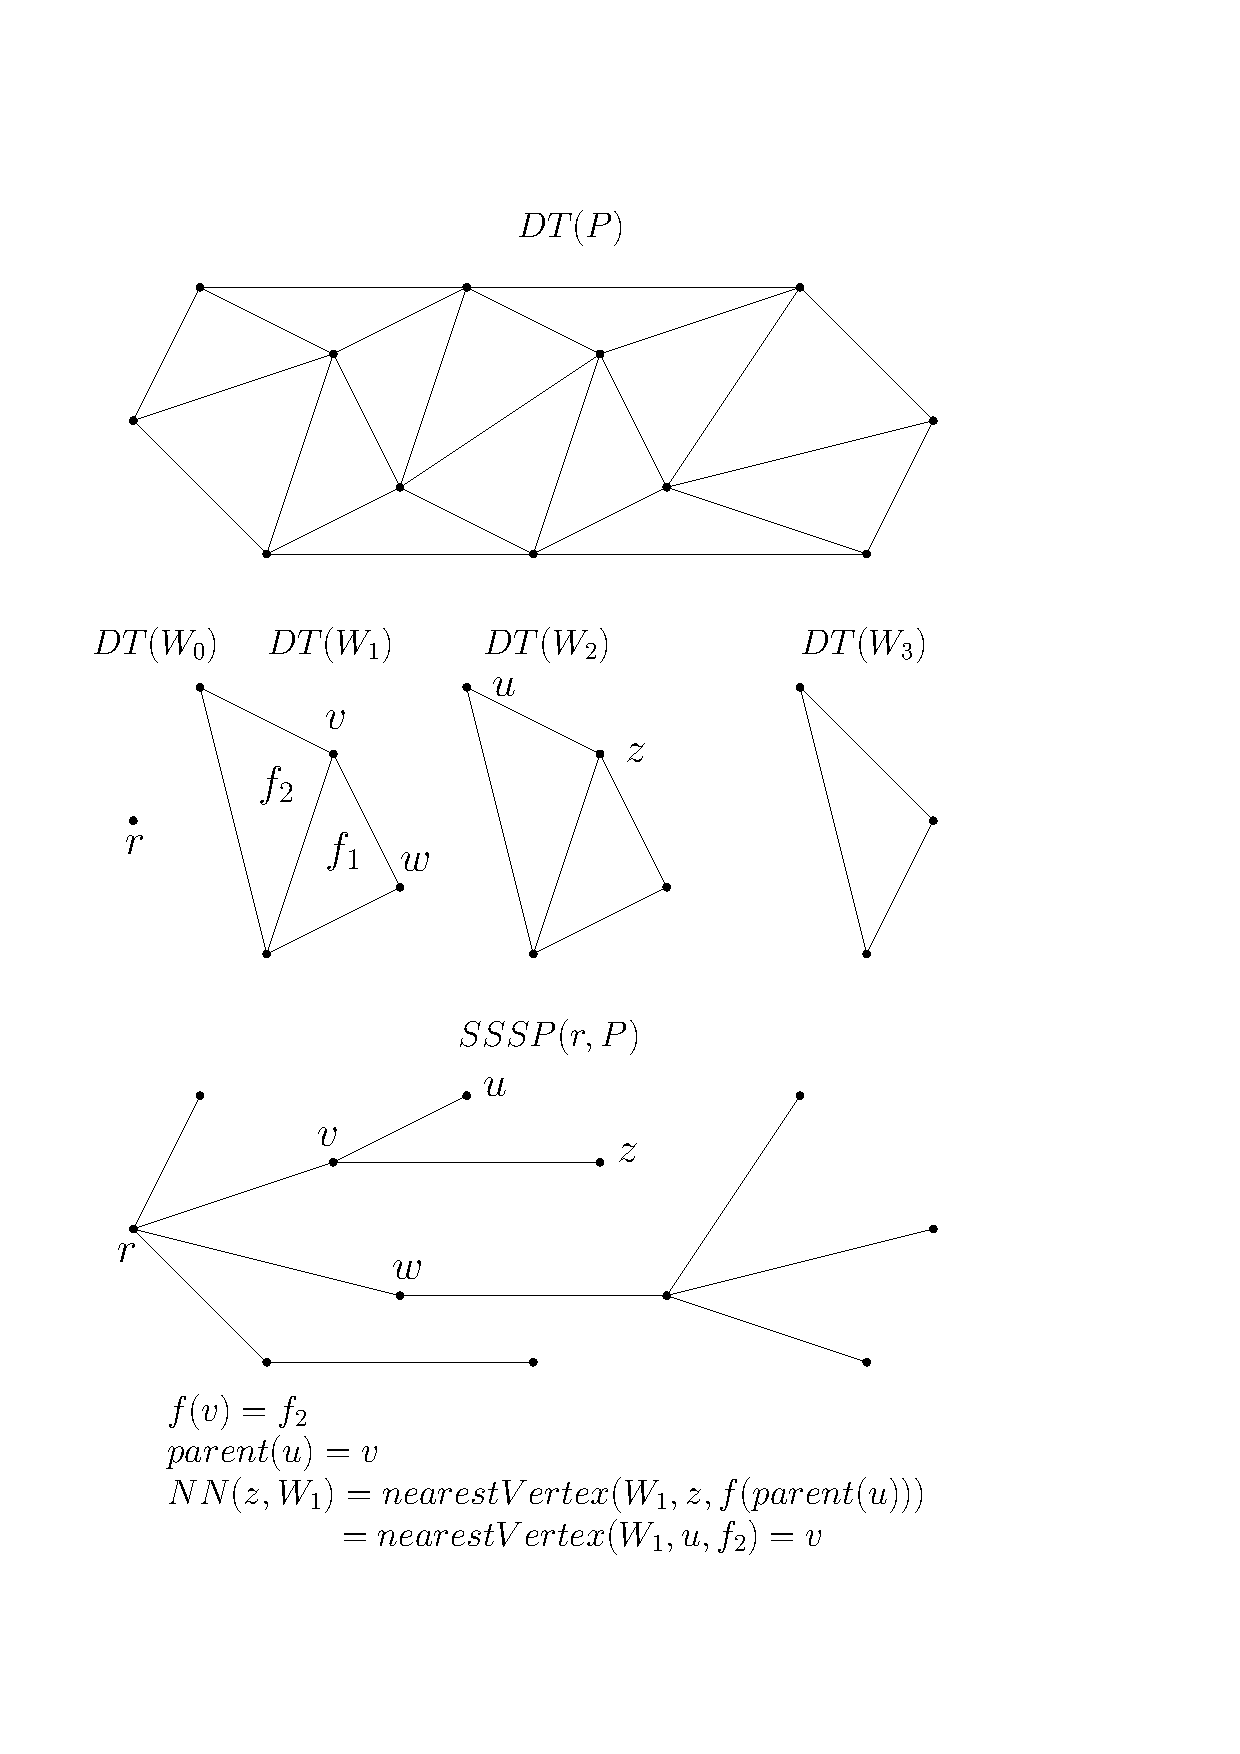
\includegraphics[scale=0.6]{pics/pointsToFaceHandlers-all.pdf}}
\caption{Ko gradimo množico $W_2$, pri $v$ preverimo vse njegove sosede v DT(P), ki še niso bile obiskane in dodane v drevo. To je edino vozlišče $u$, ki ga dodamo v $W_2$ in $Q$. Ker je $v$ sosed $u$ in del $DT(W_1)$, uporabimo njegovo lice $f_2$ kot začetno lice pri iskanju najbližjega soseda točke $u$. $u$ nato dodamo v drevo, njegov starš pa je $v$. Ko vzamemo $u$ iz vrste in preverimo soseda $z$, pri slednjem za začetno lice uporabimo isto lice, kot smo ga uporabili pri sosedu $u$, ker je ta že dodan v $W_2$.}
\label{pointsToFace}
\end{figure}  

Povezave oziroma sosede $q$ najdemo s krožnim iteratorjem, ki ga vrne metoda \textit{incident\U vertices(q)} v DT. Ker ima DT v knjižnici CGAL poleg standardnih vozlišč še eno neskončno vozlišče, moramo takega soseda ignorirati. Za ostale sosede $p$ najprej preverimo, če je njena točka bila že obiskana. Če ni, poiščemo njenega najbližjega soseda $w$ v $W_{i-1}$ z metodo \textit{nearestVertex}, ki ji kot argument podamo $p$ in lice $f$. Če $|pw|\le 1$, ustvarimo objekt tipa \textit{shared\U ptr\textless Point\U 2 \textgreater}, ki hrani kazalec na $w$. Ta objekt nato nastavimo kot starša točki v $p$. Točko tudi označimo kot obiskano in ji nastavimo razdaljo $i$, vozlišče $p$ pa vstavimo v seznam $W_i$. Na koncu iteracije $i$ seznam $W_{i-1}$ zamenjamo z $W_i$.

\section{Minimalna ločitev z enotskimi krogi}
\subsection{Prilagoditev drevesa SSSP}
\begin{figure}
\centerline{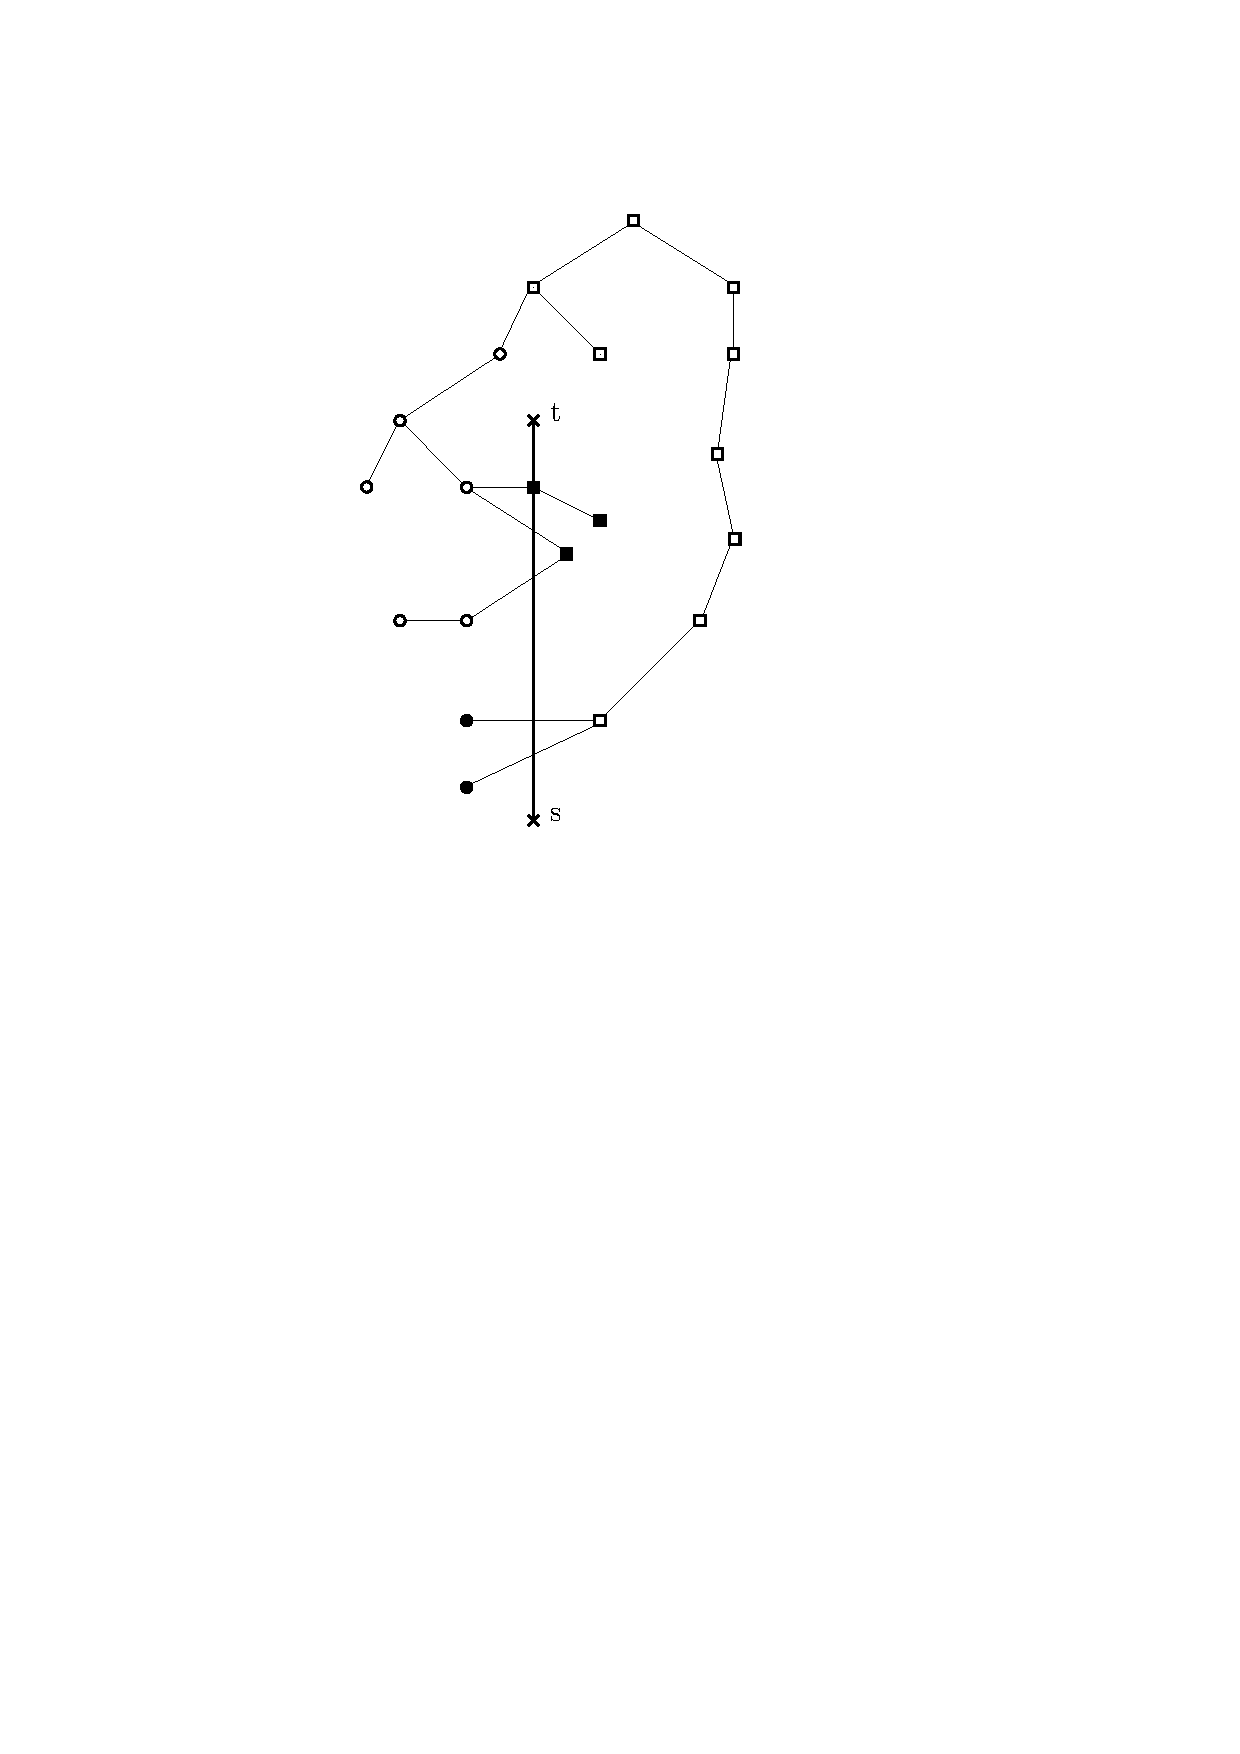
\includegraphics{pics/categorization.pdf}}
\caption{Vozlišča drevesa SSSP, ki so označena glede na skupino, v katero so uvrščena glede na daljico $\sigma$. S krogi so označena vozlišča $L0$, s polnimi krogi vozlišča $L1$, s kvadrati vozlišča $R0$ in s polnimi kvadrati vozlišča $R1$. }
\label{categorization}
\end{figure}

Pri uporabi prvega konstruktorja SSSPTree vsem danim točkam vozlišč v DT samo nastavi kazalec na njihovega starša, ki ga hranijo kot atribut. Drugi konstruktor razreda SSSPTree sprejme kot tretji argument še daljico $\sigma$, za katero program vedno predpostavi, da je navpična in da je krajišče daljice $s$ pod krajiščem $t$. Z uporabo konstruktorja s tremi argumenti metoda za izgradnjo drevesa poleg staršev točkam nastavi še vrednosti $N[\cdot]$ v atribut $nr$ in jih kategorizira tako, da jih doda v enega od štirih seznamov tipa $vector$, ki jih razred SSSPTree hrani kot zasebne atribute. Seznami se imenujejo $L0, L1, R0, R1$, kjer je $L0$ seznam, za katerega velja $L0[i] = L_0^i$. Ti seznami kot elemente tako hranijo zopet sezname, šele ti pa dejansko hranijo točke glede na njihovo razdaljo od korena drevesa. 

Za točko $p$ izračunamo $nr$ tako, da prevzamemo vrednost $nr$ njegovega starša $q$ in jo spremenimo samo v primeru, če daljica $qp$ seka $\sigma$. Za to uporabimo funkcijo v CGAL-u \textit{do\U intersect(seg1, seg2)}. Ker obstaja možnost, da $p$ ali $q$ ležita na daljici $st$ ali sta kolinearna s krajiščema $\sigma$ (ker je $\sigma$ vedno navpična daljica, to pomeni, da imajo vse tri enako vrednost koordinate $y$), je potrebno definirati, kaj storiti v takem primeru. Za točke s tako lego vedno določimo, da so desno od $\sigma$.  V primeru, da $p$ leži na $\sigma$, moramo zato za spremembo njenega atributa $nr$ poleg presečišč preveriti tudi, da se $q$ in $p$ nahajata na različni strani. $p.nr\neq q.nr$, kjer $p\in \sigma$, velja torej natanko takrat, ko se $q$ nahaja levo od $p$. S tem dodatnim pogojem zagotovimo konsistentno obnašanje algoritma (glej tudi sliko~\ref{pq-left-right}).

\begin{figure}[htp]
\centerline{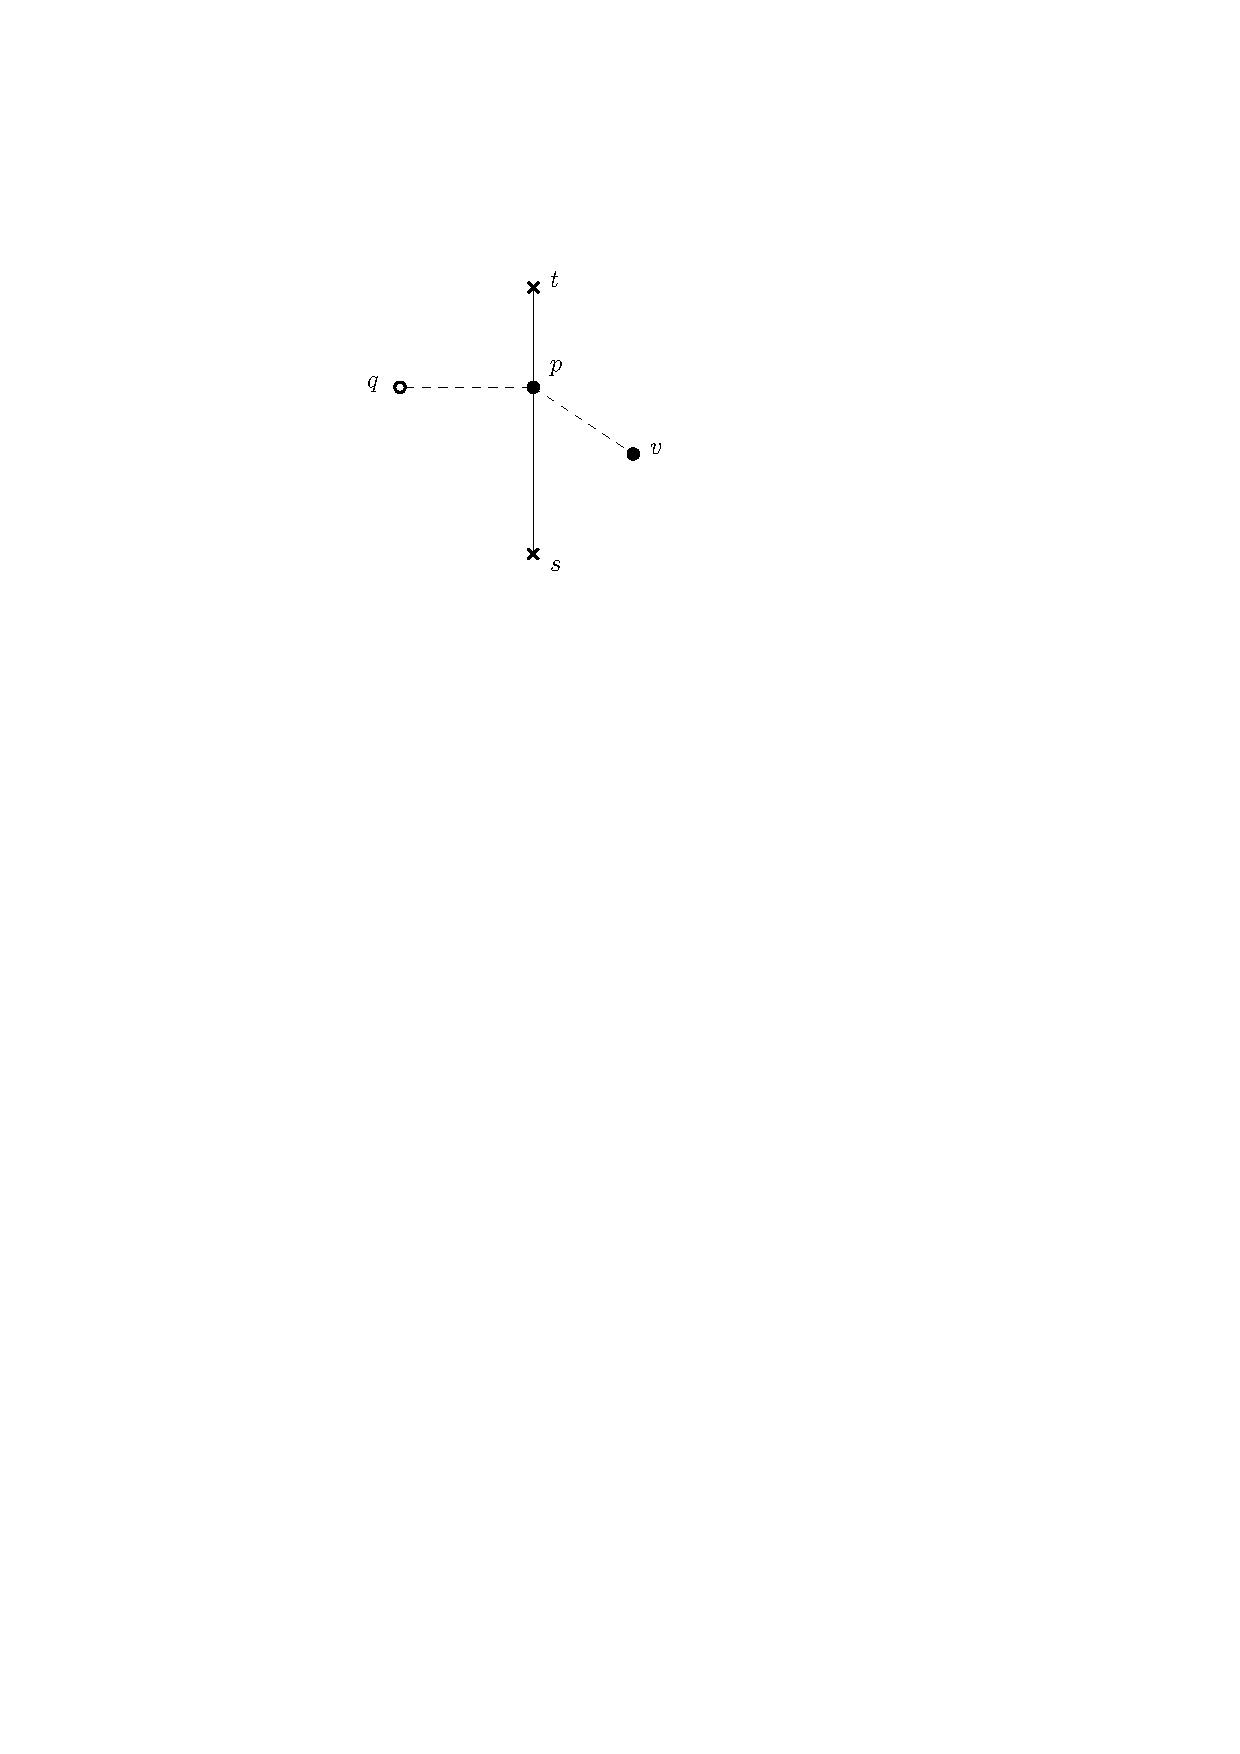
\includegraphics[scale=1]{pics/nrSideExample.pdf}}
\caption{Pri računanju vrednosti atributa \textit{nr} moramo za vsako točko in njenega starša preveriti tudi orientacijo glede na $\sigma$. Pri tem sta dovoljeni samo orientacijiski vrednosti -1 in 1, 0 (kolinearnost) pa moramo vedno obravnavati kot levo ali desno orientacijo. V nasprotnem primeru bi $p$ in $v$ imela različni vrednosti atributa $nr$.}
\label{pq-left-right}
\end{figure}

Časovna zahtevnost izračuna števila presečišč $p.nr$ je konstantna za vsak $p\in P$. Enako velja za kategorizacijo, ki poleg $nr$ izračuna še orientacijo s predikatom \textit{on\U left}. Za dostop do podseznama, kamor vstavimo točke glede na kategorizacijo in razdaljo od korena drevesa, uporabimo operator $[\ ]$, za vstavljanje točke pa metodo \textit{push\U back(p)}. Oba zagotavljata amortizirano časovno zahtevnost $\OO(1)$. S tem, ko sproti izračunamo $N[p]$ za vsako točko drevesa in podsezname $L_i^0, L_i^1, R_i^0$ in $L_i^1$, se znebimo bloka vrstic $3-5$ v teoretičnem opisu algoritma v~\ref{fig:SSSP} in si s tem prihranimo dodatni sprehod v drevesu.

\subsection{ImagePoint - implementacija točke preslikave $\varphi$}
Odločili smo se razlikovati po tipu med navadnimi točkami in točkami preslikave (slikami) $\varphi$, definirane v poglavju~\ref{dual-chapter}. Za slike smo napisali razred \textit{ImagePoint}, ki hrani dva atributa. Prvi je slika tipa \textit{Point\texttt{\_}2}, poimenovana \textit{point}. Drugi je kazalec na točko tipa \textit{Point\texttt{\_}2}, poimenovan \textit{originalPoint}. Če \textit{point} predstavlja točko $(\varphi_1(b), \varphi_2(b))$ (glej poglavje~\ref{compact}), potem \textit{originalPoint} predstavlja točko $b$. Konstruktor razreda kot argumenta sprejme točko $b$ ter daljico $\sigma$ in s pomočjo funkcije \textit{imagePoint(Point\U 2 b, Segment\U 2 $\sigma$)} izračuna točko preslikave. Kazalec na točko v primarnem prostoru hranimo zato, da lahko iz rezultata poizvedbe nad območnim drevesom, ki hrani slike, enostavno dostopamo do primarne točke, ki nas v resnici zanima.

\subsection{Kd drevo}
Za podatkovno strukturo s poizvedbami najbližjega soseda smo sprva hoteli uporabiti VD, vendar smo se kasneje odločili za kd drevo. Razlog za to je implementacija VD v knjižnici CGAL. Ker je prostorska zahtevnost VD $\OO(n)$, bi pričakovali, da poraba prostora raste linearno z večanjem VD. Izkaže se, da je rast počasnejša od linearne, kar pomeni, da na primer 100 VD objektov z 10 točkami porabi več prostora kot 10 objektov s 100 točkami. Posledično poraba prostora ni enaka za vsak nivo drevesa, temveč z globino raste. Ko smo testirali implementacijo kd dreves v CGAL-u, smo ugotovili tudi, da je čas izgradnje strukture bistveno krajši kot pri VD. Primerjave med izradnjama obeh podatkovnih struktur (procesorski čas in poraba RAM-a) so prikazane v poglavju~\ref{Rezultati}. V poštev prav tako ne pride DT, ker je brez dobrega začetnega lica, ki ga v tem primeru ne moremo zagotoviti, pričakovana časovna zahtevnost poizvedbe s sprehodom reda $O(\sqrt{n})$.

Kot osnovo smo za poizvedbe najbližjega soseda uporabili funkcijo \textit{search} v razredu $Kd{\_}tree$, ki je namenjena območnemu iskanju. Razlog za to je, da nas po lemi~\ref{lema-ds2} v resnici ne zanima najbližji sosed, ampak poljubna točka, ki je od poizvedbene točke oddaljena največ $1$. Kot argument funkcija \textit{search} sprejme \textit{OutputIterator}, kamor se shranjujejo objekti, ki jih poizvedba vrne, in \textit{FuzzyQueryItem}, ki je v dvodimenzionalnem primeru lahko krog ali pravokotnik in določa območje iskanja. Ker iščemo natanko enega najbližjega soseda, prvi argument v našem primeru ni potreben. Tretji argument, ki je neobvezen in ga ne uporabljamo, določa stopnjo mehkosti pri aproksimacijskih poizvedbah. V naši funkciji za območno iskanje, imenovano \textit{search\U exists}, smo za območje iskanja uporabili krog tipa \textit{Fuzzy\U circle} s središčem, ki ga določa točka poizvedbe in polmerom $1$. Časovna zahtevnost funkcije \textit{search} oziroma območnega iskanja v kd drevesu je enaka $\OO(\sqrt{n} + k)$, kjer je $k$ število vrnjenih točk znotraj območja iskanja. Ker je hitrost območnega iskanja ključna v našem algoritmu, smo morali prilagoditi našo funkcijo \textit{search\U exists}. Kot smo omenili, nas v resnici namesto najbližje točke zanima le, če območje iskanja vsebuje kakšno točko. To pomeni, da lahko iskanje po kd drevesu zaključimo v tistem trenutku, ko ugotovimo, da je ta pogoj izpolnjen. Konkretno je ta pogoj izpolnjen takrat, ko za neko poddrevo ugotovimo, da se njegove točke v celoti nahajajo v območju iskanja. Naša metoda v tem primeru vrne par tipa \textit{(boolean, Point\U 2)}, kjer prva komponenta hrani logično vrednost \textit{true}, druga komponenta pa prvo točko v takem poddrevesu. Če kd drevo ne hrani nobene točke, ki ima razdaljo do poizvedbene točke manjšo od 1, potem metoda vrne par \textit{(false, Point\U 2())} (druga komponenta v tem primeru ne igra nobene vloge). S tem lahko pričakujemo, da bo poizvedba v praksi delovala dobro.

\subsection{Območno drevo}
\begin{figure}
\centerline{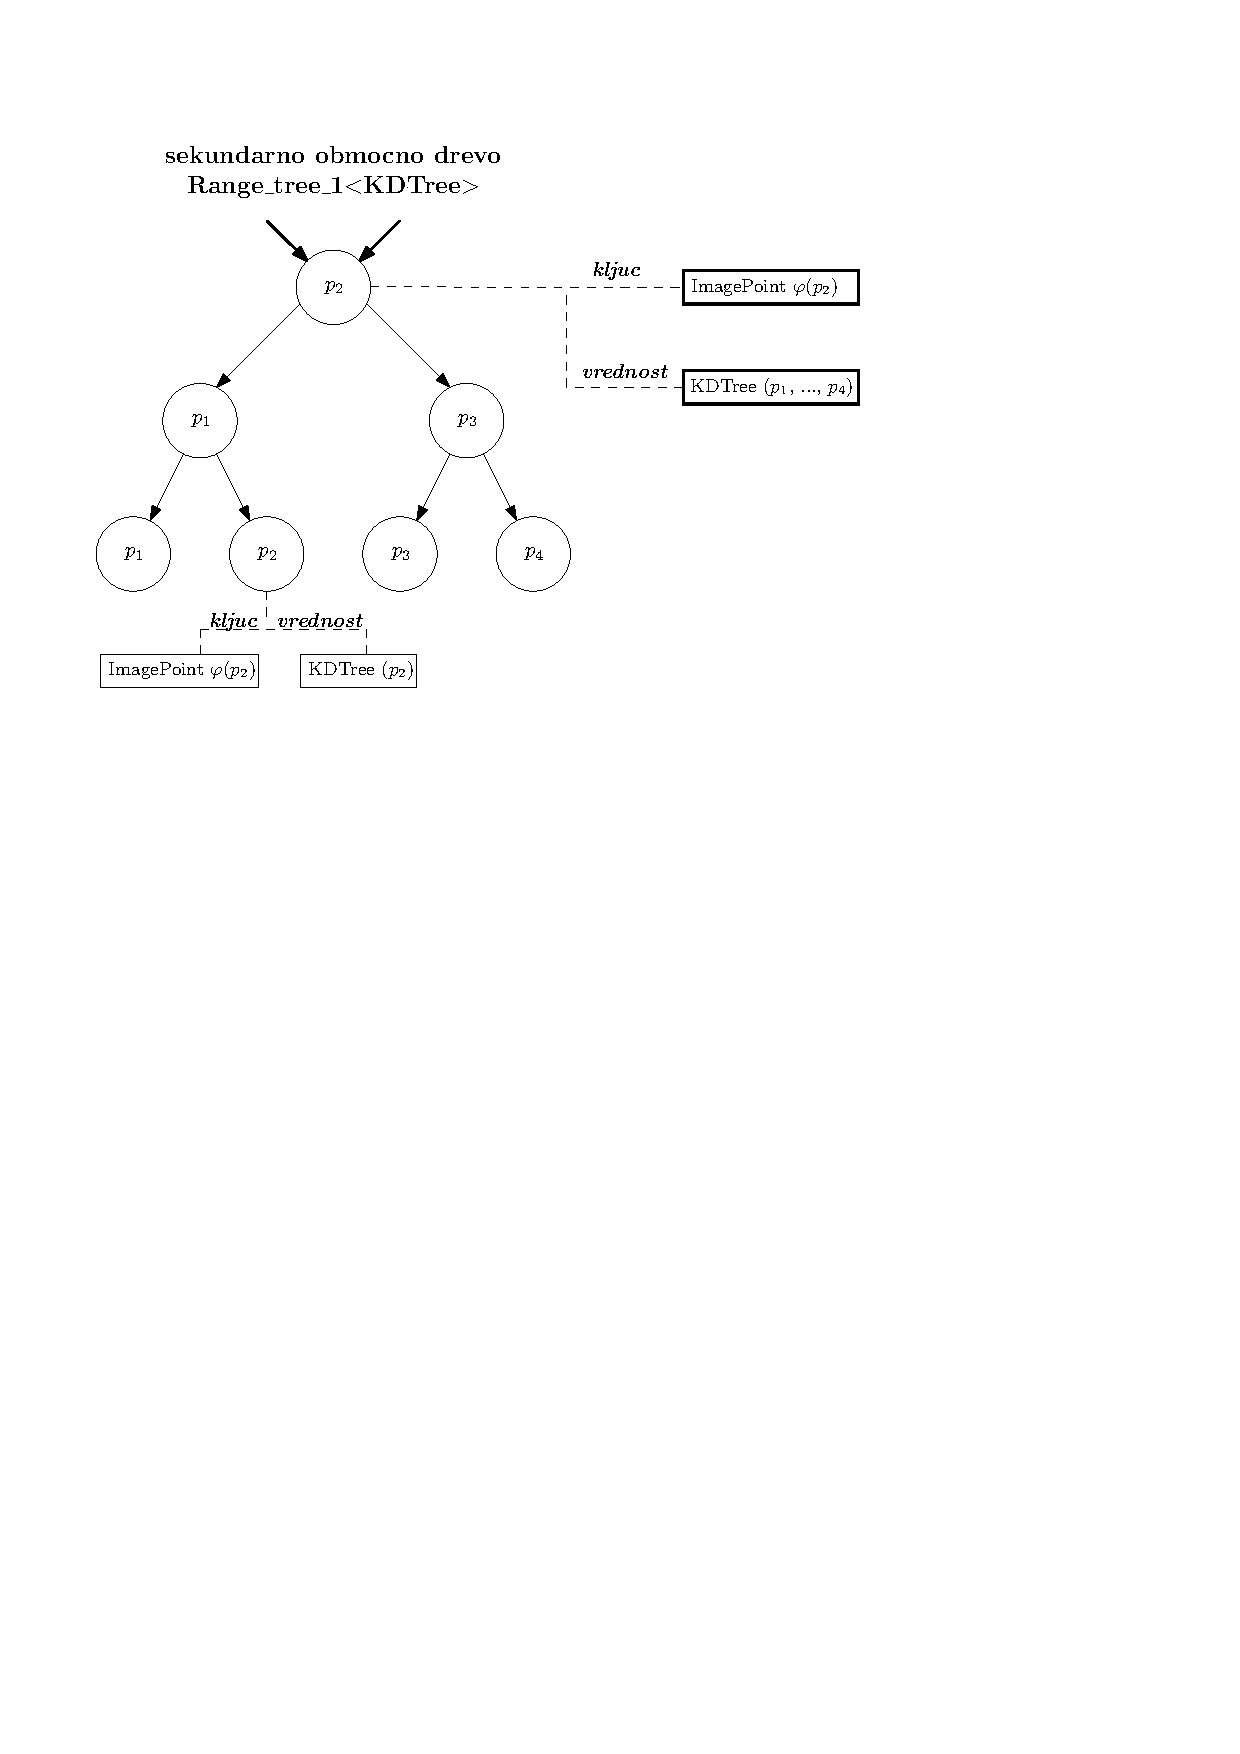
\includegraphics[scale=1]{pics/range-dual-kd-2.pdf}}
\caption{Shema zgradbe sekundarnega območnega drevesa, ki v vsakem vozlišču kot vrednost hrani kd drevo.}
\label{range-dual-kd}
\end{figure}

Za dvodimenzionalna območna drevesa smo uporabili implementacijo v knjiž\-ni\-ci CGAL, ki jo predstavlja razred \textit{Range\texttt{\_}tree\texttt{\_}2}. Vsako vozlišče hrani par, kjer prva komponenta hrani ključ, druga pa vrednost vozlišča. Slednja dodatno opisuje vozlišče in je lahko tudi odsotna, ključ pa se uporablja pri izgradnji drevesa in poizvedbah. Oba argumenta sta predlogi, kar pomeni, da moramo pri konstrukciji drevesa zanju podati konkretna tipa. 
Za ključ smo uporabili naš razred \textit{ImagePoint}, kot vrednost pa vsako vozlišče hrani svoje kd drevo. Zaradi tega smo morali vnesti nekaj sprememb v CGAL-u. Razred za značilnosti območnih dreves \textit{Range\U tree\U map\U traits\U 2} je parametriziran z modelom predstavitve dvodimenzionalnih točk tipa \textit{Point\U 2} in s tipom za vrednost vozlišča. Drevo torej kot ključ vedno uporabi objekt tipa \textit{Point\U 2 \textless K \textgreater}, kjer je $K$ model predstavitve (v naši implementaciji je ta vedno \textit{Cartesian \textless double \textgreater}). Iz razreda značilnosti smo zato odstranili prvi parameter in namesto tega samodejno nastavili tip ključa na \textit{ImagePoint}. Spremeniti smo morali tudi operatorja za primerjavo ključev v razredih \textit{C\U Compare\U 1} (za primarno drevo) in \textit{C\U Compare\U 2} (za sekundarno drevo). Funkciji kličeta predikata \textit{compare\U x} oziroma \textit{compare\U y} neposredno nad objekti obeh ključev. Ker so objekti v našem primeru tipa \textit{ImagePoint}, smo funkciji spremenili tako, da predikatoma poda atribut ključev \textit{point}, ki je tipa \textit{Point\U 2} in hrani preslikano točko.

Pri inicializaciji drevesu podamo seznam slik tipa \textit{ImagePoint} in praznih kd dreves. Nato se iterativno sprehodimo (tako kot pri preiskovanju v širino) po prvem nivoju drevesa - primarnem drevesu - s funkcijo \textit{traverse\U and\U popu\-la\-te\U with\U data}. Za vsako vozlišče pokličemo funkcijo \textit{build\U Kd\U on\U la\-yer2}, ki z rekurzivnim \textit{postorder} sprehodom za vsako vozlišče v sekundarnem drevesu, na katerega kaže vozlišče v primarnem drevesu, vstavi v (do tistega trenutka prazno) njegovo kd drevo točke, ki jih hranita kd drevesi njegovih otrok. V listih kd drevesa vsebujejo samo točko v primarnem prostoru, pri čemer je njej pripadajoča točka preslikave $\varphi$ uporabljena kot ključ vozlišča. Rekurzivni klic funkcije se torej kliče pred vstavljanjem točk v kd drevo. S pomočjo rekurzije je vsakemu notranjemu vozlišču v sekundarnem drevesu seznam točk v njegovem poddrevesu, ki ga potrebujemo za izgradnjo njegovega kd drevesa, direktno podan preko kd dreves njegovih otrok. Če bi kd drevesa gradili od zgoraj navzdol v sekundarnem drevesu, bi morali za vsako vozlišče narediti sprehod po njegovem poddrevesu. Primarno drevo za razliko od sekundarnih ne hrani nobenih dreves kot vrednosti v svojih vozliščih oziroma so ta prazna. Shema zgradbe sekundarnega drevesa je prikazana na sliki~\ref{range-dual-kd}.

\subsubsection{Poizvedbe v območnem drevesu}
Razredu \textit{Range\U tree\U d} smo za poizvedbe dodali funkcijo \textit{window\U que\-ry\U im\-pl\U mo\-di\-fied}, ki  kot osnovo uporablja obstoječo funkcijo v CGAL-u \textit{window\U que\-ry\U impl}. Argumenta funkcije sta interval $I$ in točka $q$, ki jo uporabimo za poizvedbe najbližjega soseda v kd drevesih. Interval $I$ je odvisen od $\varphi (a)$ in je zaprt. Metoda vrne par vrednosti, kjer je prva logičnega tipa, druga pa tipa \textit{Point\U 2}. Pri originalni CGAL metodi sta argumenta interval $I$ in množica $it$, kamor se shranjujejo vsi rezultati območne poizvedbe.

Če za vozlišče $w$ v primarnem drevesu ugotovimo, da njegovo celotno poddrevo ustreza pogojem poizvedbe, nadaljujemo s preiskovanjem v njegovem sekundarnem drevesu. Če za vozlišče $v$ v sekundarnem vozlišču ugotovimo, da so vsa vozlišča v njegovem poddrevesu vsebovana v intervalu $I$, ne dodamo vso poddrevo v rezultat, kot je to storjeno v izvirni metodi, temveč opravimo še poizvedbo najbližjega soseda (z območnim iskanjem) točke $a$ v kd drevesu vozlišča $v$. Če nas poizvedba nad območnim drevesom pripelje do lista primarnega ali sekundarnega drevesa, potem preverimo, če je to vozlišče vsebovano v intervalu $I$. Če je temu tako, primarno točko, iz katere izhaja točka preslikave $\varphi$, ki predstavlja ključ vozlišča $w$, vrnemo kot rezultat.

Interval $I$ je poleg slike $\varphi (a)$ odvisen tudi od tega, ali v drevesu iščemo tako točko $b$, da $ab$ seka $\sigma$ ali ne. Če ja, potem je območje iskanja drugi kvadrant v $\varphi$-ravnini (glej sliko~\ref{dualp2}), sicer sta to prvi in tretji kvadrant. Za te potrebe smo napisali metodi \textit{rangeTree\U query} in \textit{rangeTree\U query\U complement}. Pri prvi je iz točke poizvedbe $a$ interval zgrajen kot pravokotnik s spodnjim levim ogliščem $(a.x, -\infty)$ in zgornjim desnim ogliščem $(\infty, a.y)$. Pri drugi metodi sta zgrajena dva intervala: prvi ima za levo krajišče točko $(-\infty, -\infty)$ in za desno krajišče točko $a$, drugi pa za levo krajišče točko $a$, za desno pa točko $(\infty, \infty)$. Najprej se naredi poizvedba s prvim intervalom in le če slednja ne vrne nobenega rezultata, se poizvedba naredi tudi z drugim intervalom.
\subsection{Celotna struktura algoritma}

\begin{figure}[htp]
\begin{center}
\ovalbox{~~~~
\begin{varwidth}{\linewidth}
\begin{codebox}
    \Procname{\proc{Psevdokoda glavnega algoritma}($begin, end, \sigma$)}
    \li $\best \gets$ (\const{null}, \const{null}, \const{max value})
    \zi // izračunaj DT
    \li $ssspTree(begin, end, \sigma)$
    \li \For $r\in P$ \Do
    	\li $ssspTree.createTreeFromRoot(r)$
    	\li $L0 \gets ssspTree.getL0()$
    	\zi // podobno za $L1, R0, R1$
    	\li $i \gets 1$
    	\li $maxDist \gets size(l0)$
    	\li \While $2i< \best \mbox{ in } 2i \leq maxDist$ \Do
    		\li $result \gets nnSeparation(L0, L1, R0, R1, i)$
    		\li \If $result[2] < best[2]$ \Then
    			\li $best \gets result$
    			\li \kw{break}
    		\End
    		\li $result \gets rangeSeparation(L0, L1, R0, R1, i, \sigma)$
    		\li \If $result[2] < best[2]$ \Then
    			\li $best \gets result$
    			\li \kw{break}
    		\End
    		\li $i++$
    	\End
    	\\ \> // resetiraj vrednosti atributov v točkah DT
  		\li $ssspTree.resetTree()$
  	\End
    \li \Return makeCycle(best)
    \\[-2mm]
\end{codebox}
\end{varwidth}
~~~~}\end{center}
\caption{Celotna shema algoritma za minimalno ločitev.}
\label{fig:sep-overall-1}
\end{figure}


\begin{figure}[htp]
\begin{center}
\ovalbox{~~~~
\begin{varwidth}{\linewidth}
\begin{codebox}
    \Procname{\proc{nnSeparation}($L0, L1, R0, R1, i$)}
    \li $L_i^0 \gets L0[i]$
    \li $L_{i-1}^0 \gets L0[i-1]$
    \\ // podobno za $L1, R0, R1$
    \li $groups \gets [L_{i-1}^0, L_{i}^1, L_{i}^0, L_{i-1}^1, R_{i-1}^0, R_{i}^1, R_{i}^0, R_{i-1}^1]$
    \li $pairs \gets [(0,1), (2, 3), (4, 5), (6, 7), (1, 2), (5, 6)]$
    \li \For $pair\in pairs$ \Do
    	\li $A \gets groups$ $[pair.first]$
       	\li $B \gets groups$ $[pair.second]$
       	\li \If $A$ neprazen in $B$ neprazen \Then
       		\li $kdtree(B.begin(), B.end())$
       		\li \For $a\in A$ \Do 
       			\li $result \gets kdtree.customSearch(a)$
       			\li \If $(result[0])$ \Then
       				\li $nearest \gets result[1]$
       				\li \Return $(a, nearest,$
       				 \Indentmore \Indentmore
       				\zi $dist(a) + dist(nearest))$ \End \End
       			\End
       		\End
       	\End
    \End
    \li \Return (\const{null}, \const{null}, \const{max value})
    \\[-2mm]
\end{codebox}
\end{varwidth}
~~~~}\end{center}
\caption{Pomožna funkcija algoritma za iskanje minimalne ločitve nad ustreznimi pari s kd drevesom.}
\label{fig:sep-overall-2}
\end{figure}

Program kot prvi argument sprejme tekstovno datoteko, ki vsebuje po eno točko v vsaki vrstici kot par koordinat. Kot drugi argument je podano začetno krajišče daljice $\sigma$, točka $s$, kot tretji pa točka $t$ kot končno krajišče daljice. Veljati mora $s.x == t.x$. Nato se pokliče glavna metoda programa, v kateri se izvedejo vsi izračuni in ki se okvirno ujema s sliko~\ref{fig:FULL}.

Najprej se inicializira objekt SSSPTree, ki v konstruktorju zgradi DT. Za vsako točko $r\in P$ se nato zgradi drevo s korenom $r$. Iz drevesa dobimo ven štiri sezname $L0, L1, R0, R1$, kjer so točke organizirane po njihovih razudaljah do korena $r$. V \textit{while} zanki nato preverimo kandidate v istem vrstnem redu, kot so nanizani v sliki~\ref{fig:FULL}. Za kandidate na isti strani daljice $\sigma$ se pokliče metoda \textit{nnSeparation}, za ostale pa \textit{rangeSeparation}.

V metodi \textit{nnSeparation} za vse pare množic točk $(S_1, S_2)$ na isti strani daljice $\sigma$ in ki tvorijo cikel dolžine $2i$ zgradimo kd drevo nad $S_2$, za vsako točko $p\in S_1$ pa v drevesu z območnim iskanjem poiščemo prvo točko $q$, ki je od $p$ oddaljena za največ $1$. To naredimo z našo metodo \textit{search\U exists}. Preprosta optimizacija, ki smo jo dodali v algoritem, je ta, da vnaprej zavržemo tiste pare, pri katerih je ena od množic prazna. S tem bistveno pohitrimo algoritem (glej poglavje~\ref{Rezultati}), saj nima smisla delati poizvedbe nad praznim drevesom ali zgraditi drevesa, nad katerim ne bomo naredili nobene poizvedbe.

V \textit{rangeSeparation} preverimo pare v sledečem vrstnem redu: $L_i^0\times R_{i-1}^0$, $L_i^1\times R_{i-1}^0$, $L_i^1\times R_{i-1}^1$, $L_i^0\times R_{i-1}^1$, $L_{i-1}^0\times R_{i}^0$, $L_{i-1}^0\times R_{i}^1$, $L_{i-1}^1\times R_{i}^0$, $L_{i-1}^1\times R_{i}^1$, $L_{i}^0\times R_{i}^0$, $L_{i}^0\times R_{i}^1$, $L_{i}^1\times R_{i}^0$, $L_{i}^1\times R_{i}^1$. Območnih dreves ne gradimo za vsak par posebej, temveč enkrat za vsako od množic $R_{i-1}^0, R_{i-1}^1, R_{i}^0, R_{i}^1$, če je to potrebno. Tudi tukaj namreč ne preverjamo parov, pri katerih je ena od množic prazna. Za pare, kjer iščemo kandidate, ki sekajo $\sigma$, uporabimo metodo \textit{rangeTree\U query}, za kandidate, ki ne sekajo $\sigma$, pa metodo \textit{rangeTree\U query\U complement}. Na koncu z metodo \textit{nnSeparation} preverimo še zadnja dva para $L_i^0\times L_i^1$ in $R_i^0\times R_i^1$. S takim zaporedjem parov lahko v trenutku, ko naletimo na prvi par, ki vrne neprazen rezultat, prenehamo z iskanjem z ostalimi pari, zaključimo zanko in s tem iskanje cikla za koren $r$.

\subsection{Izgradnja minimalnega cikla}
Ko dobimo par točk $a, b\in P$, ki določata minimalno sklenjeno pot, ki ločuje točki $s$ in $t$, v seznam shranimo vse točke, ki tvorijo cikel. S pomočjo funkcije $getParent()$ lahko za vsako točko $p$ v drevesu $SSSP(r, P)$ dobimo njegovega starša in s tem pot $T_r[p]$ v obratnem vrstnem redu (z začetkom pri točki $p$ in koncem pri točki $r$), ki jo označimo kot $T_r^{-1}[p]$. Pot $T_r[p]$ brez točke $r$ označimo s $T_{r-1}[p]$. Cikel lahko potem dobimo z združitvijo dveh poti $T_r^{-1}[a] + T_{r-1}[b]$, ki se vedno stikata v natanko eni točki, tj. korenu drevesa. Z drugimi besedami: najmanjši skupni prednik (ang. \textit{lowest common ancestor}) točk $a$ in $b$ v drevesu najkrajših poti $SSSP(r, P)$ je vedno $r$. Če to ne bi veljalo in bi bil njun najmanjši skupni prednik točka $r^\star$, bi potem obstajal krajši cikel v drevesu $SSSP(r^\star, P)$, kjer bi $a$ in $b$ določala minimalno sklenjeno pot in bi bil njun najmanjši skupni prednik zopet točka $r^\star$. Z združitvijo obeh poti dobimo pot $(a,...,r,...b)$. Vrnjen seznam predstavlja cikel, v katerem je začetna točka shranjena samo enkrat. Za dolžino najbolj optimalne poti se do konca izvajanja programa hrani vsota dolžin točk $a$ in $b$. Dolžina, ki jo program vrne kot rezultat, je povečana za 1 zaradi povezave $ab$. 


\chapter{Eksperimenti in rezultati}
\label{Rezultati}
Eksperimente smo izvedli na prenosnem računalniku z operacijskim sistemom Windows 10, procesorjem CPU i7-6700HQ z 2,6 Ghz in 8GB spomina. Za vizualizacijo domen, vhodnih podatkov in rezultatov smo napisali skripte v programskem jeziku \textit{python} in pri tem uporabili knjižnico \textit{Matplotlib}. Vsi časi v poročanih tabelah uporabljajo sekundo kot enoto, pri tabelah s porabo prostora pa je enota MB.
\section{Uporaba kd dreves namesto VD}

\begin{table}
\begin{center}
\begin{tabular}{l|l|l|l|l|l|l}
\hline
število točk & 50k & 100k & 250k & 500k & 750k & 1mio \\ \hline \hline
CPU(VD) [s] & 0,0859 & 0,196 & 0,562 & 1,2667 & 2,0495 & 2,9304 \\ \hline
CPU(kd drevo) [s] & 0,0025 & 0,0047 & 0,0126 & 0,025 & 0,0375 & 0,0497
\end{tabular}
\caption{Povprečni čas izradnje VD in kd drevesa v sekundah.}
\label{cpu-compare}
\end{center}
\end{table}

\begin{table}
\begin{center}
\begin{tabular}{l|l|l|l|l|l|l}
število točk & 50k & 100k & 250k & 500k & 750k & 1mio \\ \hline \hline
RAM(VD) [mb] & 7.2 & 14.4 & 34.3 & 68.9 & 103.6 & 137.9 \\ \hline
RAM(kd drevo) [mb] & 1.9 & 3.8 & 9.5 & 19 & 28.5 & 38.1
\end{tabular}
\caption{Velikost prostora v megabajtih, ki ga zasede en objekt VD v primerjavi z enim objektom kd drevesa.}
\label{ram_compare}
\end{center}
\end{table}

Kot strukturo za iskanje najbližjega soseda znotraj območnega drevesa smo prvotno hoteli uporabiti VD, a smo kmalu prišli do spoznanja, da njegova implementacija v CGAL-u ni dovolj ustrezna. Prva težava, ki smo jo že omenili, je časovna zahtevnost iskanja najbližjega soseda, ki je enaka $\OO(\sqrt{n})$. Za prepočasno se je izkazala tudi sama izgradnja strukture. Primerjava časov izgradnje VD in kd dreves je za različno število točk prikazana v tabeli~\ref{cpu-compare}. Testi so se izvedli na prenosniku s procesorjem i5-5200U z 2,20Ghz, prikazani časi pa so povprečje desetih iteracij testa. Sami objekti VD v CGAL-u porabijo tudi bistveno več prostora kot kd drevesa, kar je prikazano v tabeli~\ref{ram_compare}. Glavni problem s prostorom, ki ni prikazan v tabeli, je v VD z majhnim številom točk. Območno drevo, ki hrani 100 točk, ima v korenu sekundarnega drevesa shranjeno strukturo za poizvedbe najbližjega soseda s 100 točkami. Po drugi strani ima drevo 100 listov in v vsakem je shranjena struktura z eno točko. Implementacija VD krši teoretično prostorsko zahtevnost območnega drevesa, ki temelji na tem, da vsi nivoji drevesa porabijo podobno veliko prostora. 10 VD-jev s 1000 točkami tako porabi 3,3mb prostora, 10000 VD-jev z eno točko pa kar 200mb.  

\section{Generator vhodnih podatkov}
\begin{figure}
\centerline{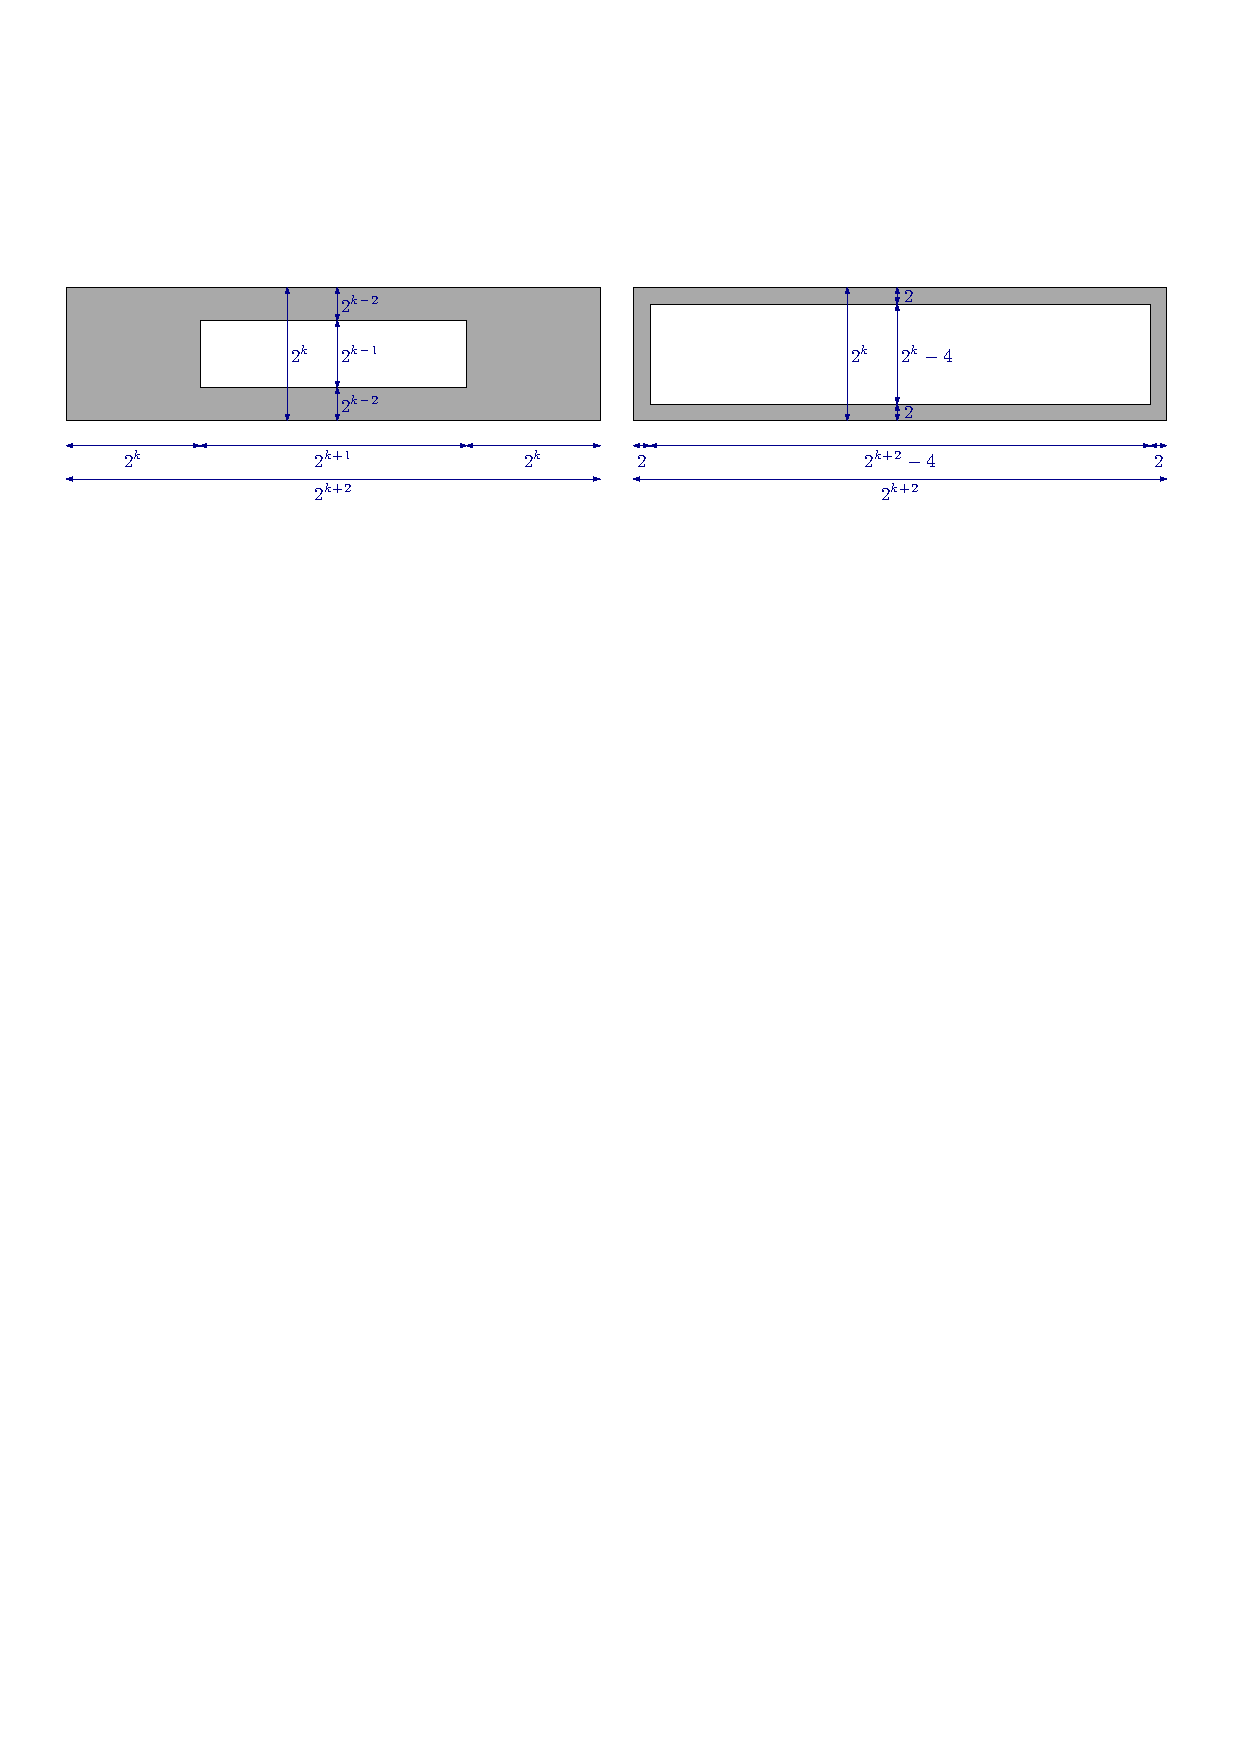
\includegraphics[scale=0.75, page=1]{pics/data_generation.pdf}}
\caption{Pravokotna domena z eno manjšo (levo) in eno večjo luknjo (desno). Prikazane so tudi velikosti oziroma razmerja velikosti med celotno domeno in luknjo.}
\label{generation1}
\end{figure}

\begin{figure}
\centerline{\includegraphics[scale=0.75, page=2]{pics/data_generation.pdf}}
\caption{Pravokotna domena s štirimi manjšimi (levo) in štirimi večjimi luknjami (desno.)}
\label{generation2}
\end{figure}

Točke smo generirali naključno znotraj sledečih poligonskih domen: pravokotnik brez lukenj, pravototnik z manjšo luknjo, pravokotnik z večjo luknjo, pravokotnik s štirimi manjšimi luknjami in pravokotnik s štirimi večjimi luknjami. Natančne dimenzije domen so prikazane na slikah ~\ref{generation1} in~\ref{generation2}. Konkretno smo uporabili domene, kjer je imel zunanji pravokotnik dimenzije $4\times 1$, $8\times 2$,\ldots, $128\times 32$. Velikost vhodnih podatkov je bila 1K, 2K, 5K, 10K, 20K in 50K točk. Podatke smo generirali enkrat in nato zapisali v tekstovno datoteko. Pri testiranju problema minimalne ločitve smo točko $s$ postavili na sredino luknje, $t$ pa vertikalno nad $s$ in zunanjim pravokotnikom. Pri domenah s štirimi luknjami smo $s$ postavili na sredino zgornje leve luknje. Prvi dve točki v tekstovni datoteki, ki hrani vhodne podatke, sta vedno obravnavani kot točki $s$ in $t$. Domen s premajhnimi luknjami nismo uporabili za problem minimalne ločitve, ker je višina lukenj manjša od $1$ in bi drevo najkrajših poti vsebovalo povezave med točkama na nasprotnih straneh luknje. S tem bi se vloga luknje izgubila in bi kot rešitev dobili trivialni cikel. 

Pri večjih domenah in manjših vhodnih podatkih je bil izziv zapolniti prostor, ki je pogoj za obstoj rešitve minimalnega problema, saj so točke bolj razpršene. Za vhodne podatke sicer nismo zahtevali pogoja, da je njihov graf $G$ povezan, smo pa želeli, da je velikost največje komponente $G$ dovolj podobna velikosti celotnega grafa $G$. S tem smo povečali možnost obstoja rešitve in dosegli, da smo dejansko testirali želeno število vhodnih podatkov. Nekatere kombinacije (na primer $1000$ točk na domeni z zunanjim pravokotnikom $128\times 32$) smo zato izpustili, pri drugih pa smo problem rešili tako, da smo za generirane točke preverili, da imajo $1 << m << k$ sosedov (točk, od katerih so oddaljene za največ $1$) med trenutnimi vhodnimi podatki. Če pogoj ni bil izpolnjen, smo generirano točko zavrgli. S spodnjo mejo smo zagotovili povezanost grafa, z zgornjo mejo pa določili intenzivnost zapolnjevanja prostora domene. Minimalno vrednost za $k$, ki še dovolj zapolni domeno tako, da je luknja obdana s točkami iz vseh strani, smo za vsako kombinacijo posebej dobili s poskušanjem različnih vrednosti. $k$ se je ponavadi gibal med $3$ in $5$ (manjši $k$ pomeni hitrejše zapolnjevanje prostora, zato smo ga uporabili pri večjih domenah). Smiselno zaporedje generiranih točk smo pri eksperimentih nevtralizirali tako, da so točke pred uporabo algoritmov naključno sortirane.

\section{Drevo najkrajših poti}
Implementacijo algoritma SSSP smo primerjali z dvema očitnima alternativnima algoritmoma za drevesa najkrajših poti. Pri prvi eksplicitno zgradimo graf $G=\GG(P)$ tako, da za vse možne pare $p, q\in P$ dodamo povezavo $pq$ v strukturo grafa, če je razdalja med $p$ in $q$ največ 1 (glej odsek~\ref{bfs-theory}). Za vsako točko iz vhodnega seznama, ki ga nespremenjenega hranimo ves čas, zgradimo vozlišče. Za vozlišče grafa smo napisali strukturo $GraphNode$, ki hrani točko tipa $Point\U 2$, kazalec na starša in sosede kot seznam indeksov, ki določajo položaj soseda/točke v vhodnem seznamu. Za vsako vozlišče preverimo razdaljo do ostalih vozlišč (brez simetričnih primerov; skupno preverimo torej $\frac{n(n-1)}{2}$ parov) in za vsak par vozlišč z razdaljo največ 1 dodamo drug drugega v seznam sosedov. Drevo najkrajših poti potem zgradimo s klasičnim algoritmom za preiskovanje v širino (glej~\ref{fig:genericBfs}). 

Kot drugo alternativo uporabimo mrežo enotskih razdalj (glej odsek~\ref{grid-chapter}). Dve točki $(x,y)$ in $(x',y')$ se nahajata v isti celici mreže natanko takrat, ko velja $(\lfloor x\rfloor ,\lfloor y\rfloor)=(\lfloor x'\rfloor ,\lfloor y'\rfloor)$. Vse točke v celici $c$ shranimo v seznam $\ell(c)$. Vse neprazne sezname $\ell(c)$ shranimo v razpršeno tabelo, v kateri je kot ključ uporabljeno spodnje levo oglišče celice. S tako strukturo nato izvedemo nekakšno preiskovanje v širino. Seznam $\ell(c)$ celice $c$ hrani točke, ki še niso bile obiskane z drevesom najkrajših poti. Ko procesiramo točko $p$ v celici $c$, moramo kot kandidate obravnavati vse ostale točke v $\ell(c)$ in točke v seznamih osmih sosednih celic. Vsaka točka, ki je sosedna $p$, je nato odstranjena iz seznama svoje celice. Enostavno se da najti primere, kjer bi bila časovna zahtevnost izgradnje drevesa kvadratična. Za vsako najkrajše drevo razpršeno tabelo zgradimo od začetka. Ker je čas, ki ga porabimo za to, zanemarljiv, čas predprocesiranja za mrežo ni prikazan med rezultati. Za seznam točk v celicah smo pri implementaciji uporabili strukturo $list$ in ne $vector$. Razlog za to je ta, da je vsaka točka slej ko prej odstranjena iz seznama svoje celice. $vector$ v C++ omogoča samo brisanje vsebine elementa seznama na $i$-tem mestu, ne pa brisanja samega elementa oziroma je časovna zahtevnost tega $O(n)$. Po drugi strani $list$ porabi nekaj več spomina, ker vsak element hrani še kazalca na prejšnji in naslednji element, ima enak čas vstavljanja elementa na konec seznama kot $vector$, vendar je časovna zahtevnost brisanja (in vstavljanja) elementa sredi seznama $O(1)$, ker samo preveže skupaj njegovega predhodnika in naslednika (velika prednost tipa \textit{vector} pred \textit{list} je sicer v tem, da je časovna zahtevnost dostopa do naključnega elementa seznama $\OO(1)$). Za razpršeno tabelo celic smo uporabili strukturo $unordered\U map$, ki kot ključ hrani par celih števil, ki predstavljajo spodnje levo oglišče celice. Za ključ smo morali definirati tudi dobro $hash$ funkcijo, odporno na trke (ang. $collisions$). Uporabili smo Cantorjevo funkcijo $\pi (k_1, k_2) = \frac{1}{2}(k_1+k_2)(k_1+k_2+1) + k_2$.

\begin{table}
\begin{center}
\begin{tabular}{l*{3}{r}}
\textbf{Brez lukenj} & \multicolumn{3}{c}{20K točk}\\						
dimenzije pravokotnika	&	$4\times 1$	&	$8\times 2$	&	$16\times 4$ \\
\hline
predprocesiranje SSSP	&	0.025	&	0.027	&	0.025		\\
povprečje za koren s SSSP	&	0.131	&	0.130	&	0.127		\\
predprocesiranje BFS 	&	25.057	&	20.433	&	17.773		\\
povprečje za koren z BFS	&	3.406	&	1.359	&	0.404		\\
grid	&	1.605	&	1.647	&	0.695	\vspace{.2cm}	\\

&	$32\times 8$	&	$64\times 16$	&	$128\times 32$	\\
\hline
predprocesiranje SSSP &	0.025	&	0.025	&	0.026 \\
povprečje za koren s SSSP &	0.126	&	0.129	&	0.136 \\
predprocesiranje BFS &	17.734	&	17.347	&	17.179 \\
povprečje za koren z BFS &	0.088	&	0.025	&	0.009 \\
grid &	0.227	&	0.089	&	0.053 \vspace{.2cm} \\
\hline
  & \multicolumn{3}{c}{50K točk}  \\						
&	$4\times 1$	&	$8\times 2$	&	$16\times 4$ \\
\hline
predprocesiranje SSSP	&	0.091	&	0.091	&	0.070		\\
povprečje za koren s SSSP	&	0.592	&	0.562	&	0.375		\\
predprocesiranje BFS	&	$>$3min	&	159.812	&	144.965		\\
povprečje za koren z BFS	& omejitev RAM-a & 9.378	&	2.789		\\
grid				&	11.567	&	13.660	&	4.592	\\

&	$32\times 8$	&	$64\times 16$	&	$128\times 32$	\\
\hline
predprocesiranje SSSP &	0.071	&	0.070	&	0.069 \\
povprečje za koren s SSSP &	0.377	&	0.372	&	0.366 \\
predprocesiranje BFS &	140.404	&	131.854	&	132.475 \\
povprečje za koren z BFS &	0.584	&	0.144	&	0.044 \\
grid &	1.346	&	0.432	&	0.187
\end{tabular}
\caption{Časi za izgradnjo dreves najkrajših poti v pravokotnih domenah brez lukenj.}
\label{table1}
\end{center}
\end{table}



\begin{table}
\begin{center}
\begin{tabular}{l*{3}{r}}
\textbf{Ena manjša luknja} & \multicolumn{3}{c}{10K točk}\\						
dimenzije pravokotnika	&	$4\times 1$	&	$8\times 2$	&	$16\times 4$		\\
\hline
predprocesiranje SSSP	&	0.021	&	0.012	&	0.012		\\
povprečje za koren s SSSP	&	0.104	&	0.059	&	0.060		\\
predprocesiranje BFS	&	8.500	&	4.300	&	4.100		\\
povprečje za koren z BFS	&	1.183	&	0.318	&	0.091		\\
grid	&	0.486	&	0.513	&	0.168  \vspace{.2cm}	\\
&	$32\times 8$	&	$64\times 16$	&	$128\times 32$ \\
predprocesiranje SSSP &	0.012	&	0.012	&	0.012 \\
povprečje za koren s SSSP &	0.061	&	0.064	&	0.070 \\
predprocesiranje BFS &	4.100	&	4.000	&	4.000 \\
povprečje za koren z BFS &	0.026	&	0.008	&	0.003 \\
grid &	0.072	&	0.035	&	0.026\vspace{.2cm} \\
\hline
  & \multicolumn{3}{c}{20K točk}\\
  &	$4\times 1$	&	$8\times 2$	&	$16\times 4$		\\  			
\hline
predprocesiranje SSSP	&	0.027	&	0.026	&	0.025	\\
povprečje za koren s SSSP	&	0.142	&	0.137	&	0.136	\\
predprocesiranje BFS	&	24.813	&	19.817	&	18.396	\\
povprečje za koren z BFS	&	3.253	&	1.328	&	0.467	\\
grid				&	2.181	&	2.627	&	0.668	\\
&	$32\times 8$	&	$64\times 16$	&	$128\times 32$ \\
predprocesiranje SSSP &	0.025	&	0.025	&	0.025	\\
povprečje za koren s SSSP &	0.136	&	0.138	&	0.145	\\
predprocesiranje BFS &	17.976	&	17.542	&	17.313	\\
povprečje za koren z BFS &	0.108	&	0.031	&	0.011	\\
grid &	0.262	&	0.104	&	0.060 
\end{tabular}
\caption{Časi za izgradnjo dreves najkrajših poti v pravokotnih domenah z eno manjšo luknjo.}
\label{table2}
\end{center}
\end{table}

\begin{table}
\begin{center}
\begin{tabular}{l*{3}{r}}
\textbf{Štiri manjše luknje} & \multicolumn{3}{c}{10K točk} \\
dimenzije pravokotnika	&	$32\times 8$	&	$64\times 16$	&	$128\times 32$	\\						
\hline
predprocesiranje SSSP &	0.021	&	0.018	&	0.018	\\
povprečje za koren s SSSP	&	0.056	&	0.058	&	0.064	\\
predprocesiranje BFS	&	6.291	&	6.102	&	6.364	\\
povprečje za koren z BFS	&	0.033	&	0.010	&	0.004	\\
grid				&	0.064	&	0.031	&	0.023	\\
\hline
& \multicolumn{3}{c}{20K točk} \\
\hline
predprocesiranje SSSP &  0.027	&	0.026	&	0.026 \\
povprečje za koren s SSSP &	0.125	&	0.126	&	0.131 \\
predprocesiranje BFS &	18.325	&	17.887	&	17.256	\\
povprečje za koren z BFS & 0.102	&	0.031	&	0.010 \\
grid &	0.230	&	0.096	&	0.055 
\end{tabular}
\caption{Časi za najkrajše poti v pravokotnikih s štirimi manjšimi luknjami.}
\label{table4}
\end{center}
\end{table}


\begin{table}
\begin{center}
\begin{tabular}{l*{3}{r}}
\textbf{Štiri večje luknje} & \multicolumn{3}{c}{5K točk} \\
dimenzije pravokotnika	&	$32\times 8$	&	$64\times 16$	&	$128\times 32$ \\						
\hline
predprocesiranje SSSP	&	0.007	&	0.009	&	0.009	\\
povprečje za koren s SSSP	&	0.027	&	0.028	&	0.026	\\
predprocesiranje BFS	&	1.420	&	1.420	&	1.390	\\
povprečje za koren z BFS	&	0.007	&	0.003	&	0.002	\\
grid				&	0.019	&	0.013	&	0.010	\\
\hline
& \multicolumn{3}{c}{10K točk} \\
\hline
predprocesiranje SSSP &	0.012	&	0.018	&	0.019	\\
povprečje za koren s SSSP &	0.057	&	0.054	&	0.053	\\
predprocesiranje BFS &	5.740	&	5.660	&	5.720	\\
povprečje za koren z BFS &	0.028	&	0.013	&	0.007	\\
grid &	0.060	&	0.038	&	0.027 
\end{tabular}
\caption{Časi za najkrajše poti v pravokotnikih s štirimi večjimi luknjami.}
\label{table5}
\end{center}
\end{table}

\section{Minimalna ločitev}
Kot merilo uspešnosti algoritma za minimalno ločitev smo njegove rezultate primerjali z rezultati splošnega algoritma za ločevanje, opisanega v poglavju~\ref{generic-section}. Za potrebe implementacije splošnega algoritma smo razredu \textit{Point\U 2} dodali še atribut \textit{neighbours}, ki za posamezno točko hrani seznam kazalcev na njene sosede v grafu $G$. Najprej z inicializacijo objekta \textit{SSSP\-Tree} zgradimo DT(P). Nato se algoritem z iteratorjem sprehodi čez vozlišča triangulacije, pred katerih lahko dostopamo do objektov točk. Za vsako vozlišče $u$ gremo ponovno skozi iterator vozlišč, le da ima ta začetek pri trenutnem vozlišču (skupno število iteracij je torej $\frac{n\times (n-1)}{2}$). Za vsako vozlišče $v$ druge iteracije preverimo \textit{dist(u.p,v.p)} in če je ta največ 1, v seznam \textit{u.p.neighbours} dodamo kazalec na točko $v.p$. Ker se drugi iterator ne začne s prvim vozliščem, povezavo $uv$ shranimo samo enkrat.

V glavni zanki se zopet sprehodimo skozi iterator vozlišč in za vsako njegovo točko $r$ zgradimo drevo\textit{SSSP\-Tree(r)}. S tem se za vsako točko $p$ hkrati izračuna tudi število presečišč poti od $r$ do $p$ s $\sigma$ po modulu 2. Z uporabo tretjega konstrukturja razreda SSSPTree izklopimo kategorizacijo, saj tukaj ni potrebna. Čez povezave $E(G)$ se sprehodimo tako, da gremo zopet z iteratorjem čez vsa vozlišča in za vsako točko vozlišča preverimo vse njegove sosede s pomočjo seznama kazalcev.  
\begin{table}[h!]
\begin{center}
\begin{tabular}{l*{4}{r}}
\textbf{Pravokotnik 1 manjša luknja} & \multicolumn{4}{c}{2K točk}\\
dimenzije pravokotnika	&	$8\times 2$	&	$16\times 4$	&	$32\times 8$ & $64\times 16$ \\	
\hline
nov algoritem za ločevanje	&	65	&	64	&	53	&	38  \\
splošni algoritem			&	215	&	87	&	43	&	29
\end{tabular}
\caption{Časi za minimalno ločevanje z eno manjšo luknjo.}
\label{table6}
\end{center}
\end{table}

\begin{table}[h!]
\begin{center}
\begin{tabular}{l*{3}{r}}
\textbf{Pravokotnik 4 luknje} & \multicolumn{3}{c}{2K točk, manjše luknje} \\
dimenzije pravokotnika	&	$32\times 8$ &	$64\times 16$ & $128\times 32$ \\	
\hline
nov algoritem za ločevanje	&	29	&	35	&	35	\\
splošni algoritem			&	80	&	40	&	30	\\
\hline
& \multicolumn{3}{c}{5K točk, večje luknje} \\
\hline
nov algoritem za ločevanje &	413 & 451 & 388  \\
splošni algoritem &	416 & 266 & 206
\end{tabular}
\caption{Časi za minimalno ločevanje s štirimi luknjami.}
\label{table7}
\end{center}
\end{table}

\begin{figure}
\centerline{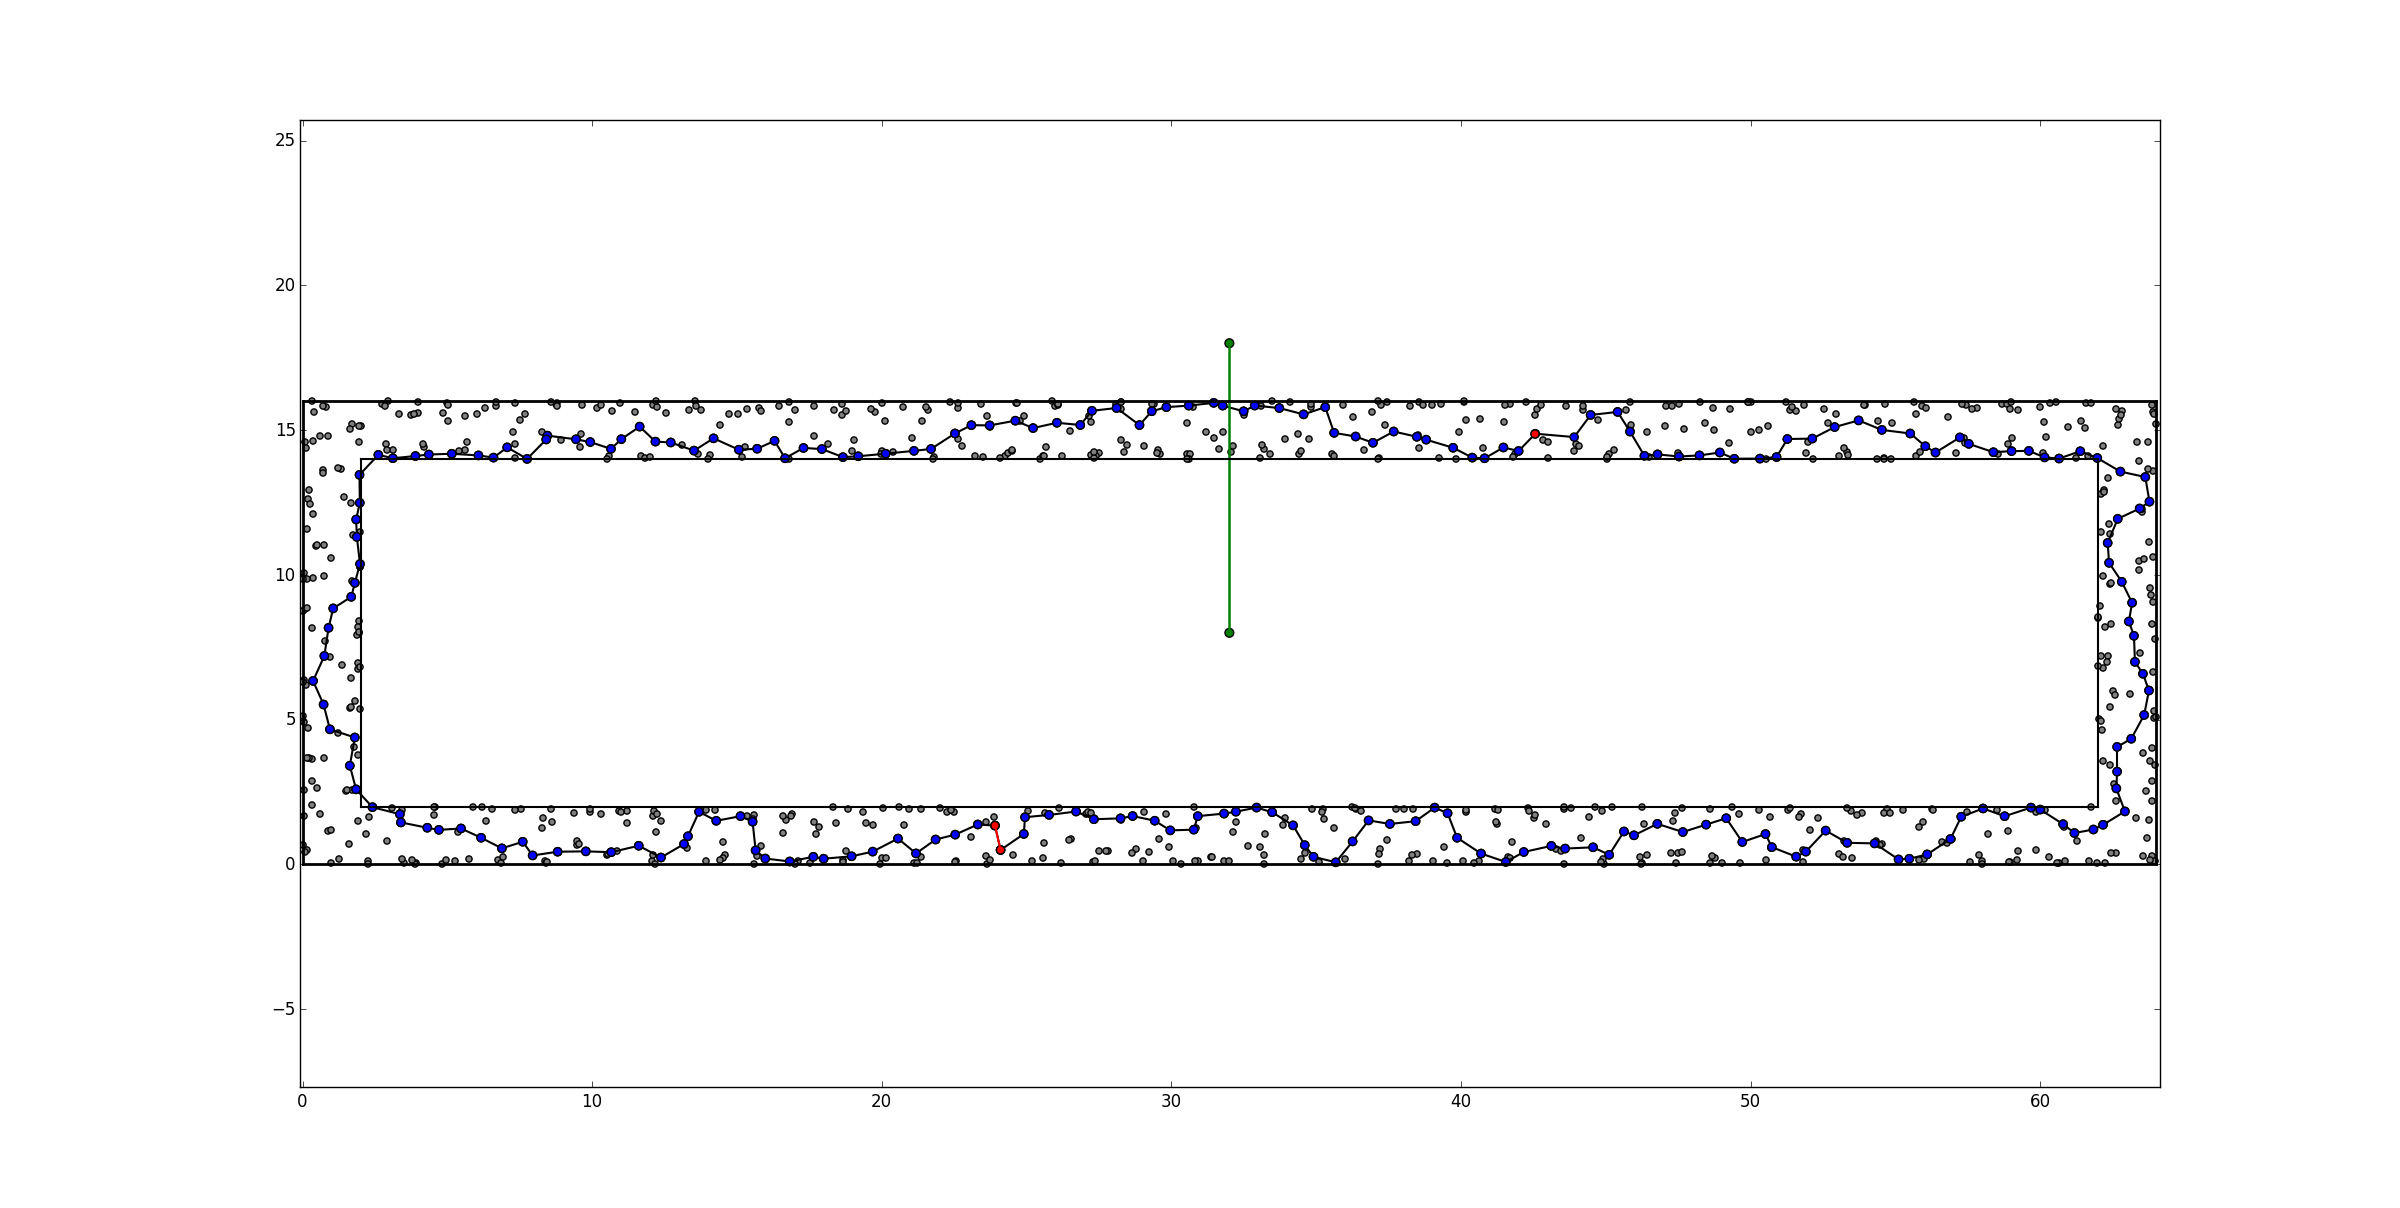
\includegraphics[scale=0.3]{pics/separation-64-1-1000-narrow-2.png}}
\caption{Primer rezultata - najkrajšega cikla - algoritma za minimalno ločitev. Modre točke so del poti cikla, samostojna rdeča točka predstavlja koren drevesa $r$, s katerim smo našli cikel, par rdečih točk $p,q$ pa z rdečo povezavo najkrajši poti od $r$ do $p$ in $r$ do $q$ združi v cikel. Zelena daljica predstavlja daljico $st$.}
\label{sep-64-1-1000-narrow}
\end{figure}

\begin{figure}
\centerline{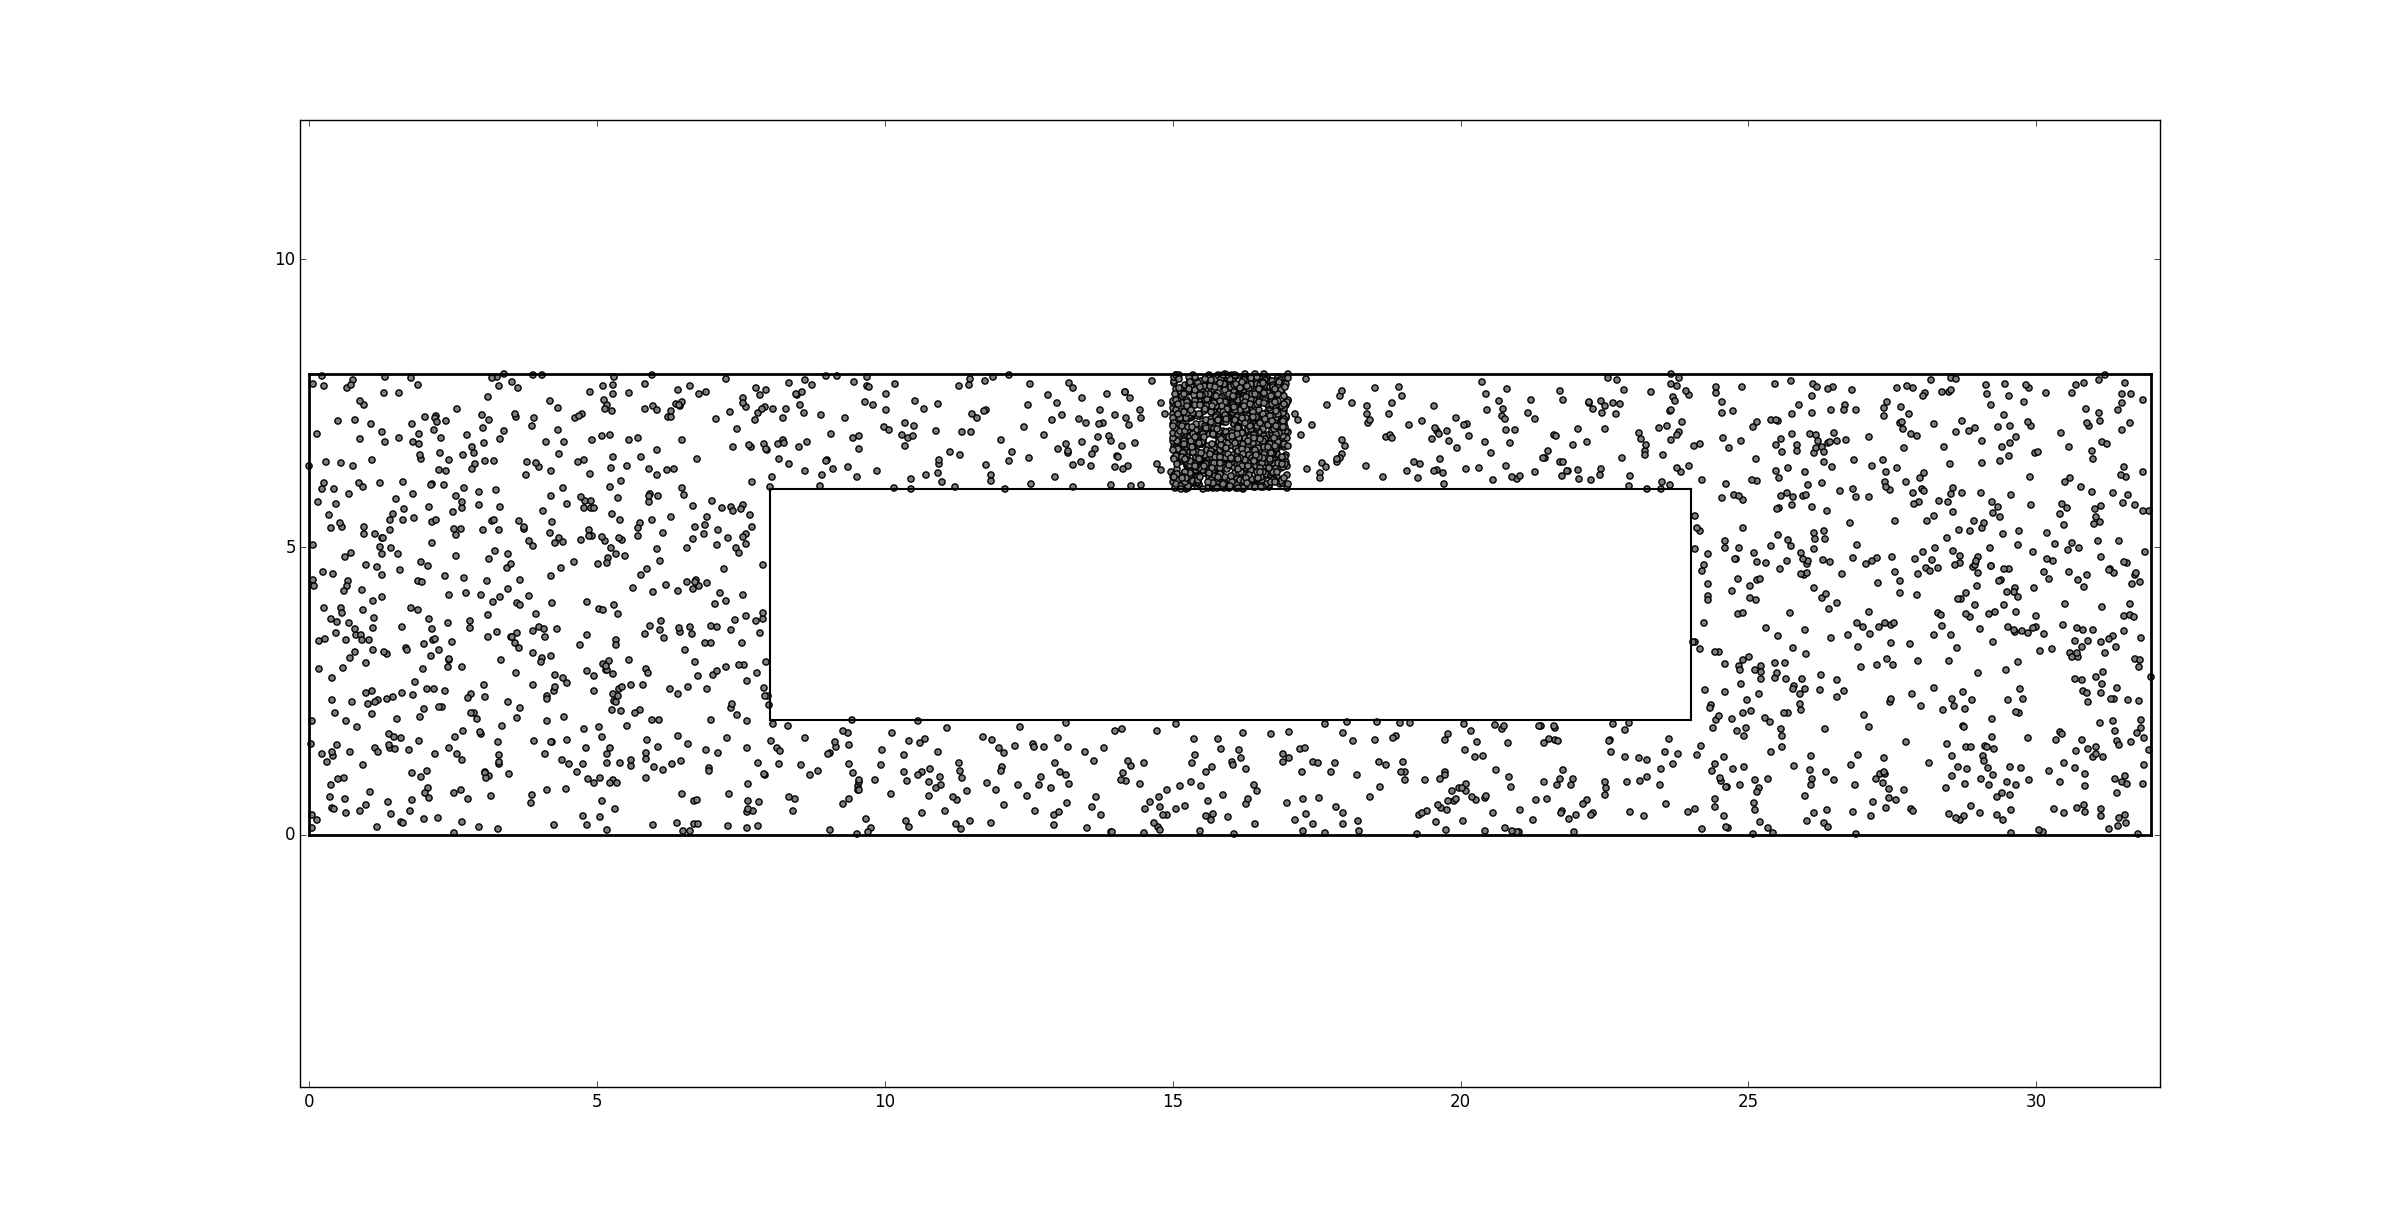
\includegraphics[scale=0.3]{pics/32-1-5000-stuffed.png}}
\caption{Primer eksperimenta, kjer se nov algoritem za ločevanje odreže bistveno bolje od splošnega algoritma. Poleg 2000 izvirnih točk smo uporabili še 1000 novih točk blizu $\sigma$, ki s tem bistveno povečajo velikost množice $E(G(P))$.}
\label{sep-stuffed}
\end{figure}

\begin{table}
\begin{center}
\begin{tabular}{l*{3}{r}}
\textbf{Brez lukenj} & \multicolumn{3}{c}{50K točk}\\						
dimenzije pravokotnika	&	$4\times 1$	&	$8\times 2$	&	$16\times 4$ \\
\hline
SSSP	&	25.2	&	22.3	&	20.1		\\
grid	&	23.2	&	22.4	&	22.2	\vspace{.2cm}	\\

&	$32\times 8$	&	$64\times 16$	&	$128\times 32$	\\
\hline
SSSP &	19.3	&	19	&	18.7 \\
BFS &	204.2	&	68.8	&	28.5 \\
grid &	21.9	&	22	&	23 \vspace{.2cm} \\
\end{tabular}
\caption{Največja poraba spomina algoritmov za najkrajše poti v domeni brez lukenj.}
\label{table-ram-tree-1}
\end{center}
\end{table}

\begin{table}
\begin{center}
\begin{tabular}{l*{3}{r}}
\textbf{Štiri večje luknje} & \multicolumn{3}{c}{5K točk}\\						
dimenzije pravokotnika	&	$32\times 8$	&	$64\times 16$	&	$128\times 32$	\\
\hline
SSSP	&	3.1	&	2.8	&	2.5		\\
BFS &	4.2	&	2.9	&	2.3 \\
grid	&	2.7	&	2.7	&	2.9	\vspace{.2cm}	\\
\hline
& \multicolumn{3}{c}{10K točk} \\
\hline
SSSP	&	5.6	 &	5.0	&	4.5		\\
BFS &	12.6	&	7.6	&	5.3 \\
grid	&	4.9	&	4.9	&	5.1	\vspace{.2cm}	\\
\end{tabular}
\caption{Največja poraba spomina algoritmov za najkrajše poti v domeni s štirimi večjimi luknjami.}
\label{table-ram-tree-2}
\end{center}
\end{table}

\begin{table}
\begin{center}
\begin{tabular}{l*{3}{r}}
\textbf{Štiri luknje} & \multicolumn{3}{c}{2K točk, manjše luknje}\\						
dimenzije pravokotnika	&	$32\times 8$	&	$64\times 16$	&	$128\times 32$	\\
\hline
nov algoritem za ločevanje	&	5.4	&	3.3	&	2		\\
splošni algoritem	&	2.9	&	2.1	&	1.8	\vspace{.2cm}	\\
\hline
& \multicolumn{3}{c}{5K točk, večje luknje} \\
\hline
nov algoritem za ločevanje	& 12.9	&	8.1	&	5.8		\\
splošni algoritem	&	8.7	&	6	&	4.2	\vspace{.2cm}	\\
\end{tabular}
\caption{Največja poraba spomina algoritmov za ločevanje v domeni s štirimi luknjami.}
\label{table-ram-sep}
\end{center}
\end{table}


\subsection{Analiza}
\label{analiza}
\begin{table}[h!]
\begin{center}
\begin{tabular}{l*{1}{c}}
(10+1)K točk, ena manjša luknja & \multicolumn{1}{c}{Časovna porast} \\
\hline
predprocesiranje SSSP &	9.7\%		\\
povprečje za koren s SSSP &	13.6\%	\\
predprocesiranje BFS & 21.9\%	\\
povprečje za koren z BFS &	56.5\% \\
grid &	25\%
\end{tabular}
\caption{Časovna porast izvajanja algoritmov za najkrajše poti, ko na območju s širino 1 10K točkam dodamo 1K novih točk.}
\label{table-increase}
\end{center}
\end{table}

Za razliko od algoritma SSSP algoritma BFS in \textit{grid} nimata nikakršne garancije za najslabši primer. Za oba lahko zgradimo takšne vhodne množice $P$, pri katerih bo njuna izvedba zelo počasna. Kot primer smo testirali $P$ s 10000 točkami v pravokotniku, ki ima dimenzije $32\times 8$ in majhno luknjo. Med krajiščema daljice $st$ smo nato v majhnem zgoščenem prostoru dodali še dodatnih 1000 točk. Širina tega prostora je $1$, tako da se število povezav v grafu $G$ bistveno poveča. Čas izvajanja je glede na prvotno instanco najmanj narastel za SSSP, največ pa za BFS (glej tabelo~\ref{table-increase}).

Podobno smo storili z algoritmom za minimalno ločevanje. Uporabili smo enako območje s 500 in 1000 dodatnimi točkami. V prvem primeru nov algoritem porabi 94 sekund (skoraj trikrat več kot brez dodatnih točk), splošni algoritem pa 435 (šestkrat več kot brez dodatnih točk). V drugem primeru nov algoritem porabi 173 sekund, splošni algoritem pa več kot 15 minut. Podobno kot pri eksperimentih z drevesi najkrajših poti se tudi tukaj nov algoritem izkaže bolje v primerih, kjer so točke bolj gosto poseljene in je med njimi več povezav. Delež dreves, ki jih moramo zgraditi, da naletimo na najkrajši cikel, je odvisen od velikosti lukenj oziroma širine območja, kjer se točke nahajajo, kar vpliva na dolžino cikla. Pri ožjih območjih je manjše število možnih poti in verjetnost, da naletimo na tako drevo, čigar koren je del najkrajšega cikla, je s tem večja. Zaradi večjih lukenj je tudi dolžina cikla večja in je tako razmerje med številom točk v ciklu in številom vseh točk večji.

Pri porabi spomina se SSSP v povprečju odreže najbolje. Splošni BFS se odreže bistveno slabše pri manjših območjih, kjer je število povezav v grafu $G$ večje. Rezultati mreže ne odstopajo znatno. Pri bolj gostih območjih se izkaže malenkost bolje kot SSSP, najmanjšo porabo pa ima pri srednje velikih območjih. Je edini od algoritmov, ki mu poraba spomina malenkost naraste pri največjem območju. To gre pripisati temu, da je zaradi enakomerne razporeditve točk potrebno zgraditi več celic v večjih območjih. 

Poraba spomina novega algoritma za ločevanje je po drugi strani nekoliko večja kot pri splošnem algoritmu. Razmerje sicer malenkost pade pri 5K točkah glede na 2K točk. Porabo spomina smo približno izmerili tudi na območju $32\times 8$ z eno luknjo in 20K točk (približno zato, ker porabe nismo merili celotni čas izvajanja, ki bi bil precej dolg). Novi algoritem porabi 45MB spomina, splošni pa 85MB. Razlog za večjo porabo spomina novega algoritma pri manj točkah najbrž leži v tem, da kljub manjši prostorski zahtevnosti nekaj dodatnega spomina zasede sama izgradnja CGAL struktur območnih in kd dreves. 
\chapter{Sklepne ugotovitve}
\label{ch4}

Čeprav se algoritem za minimalno ločevanje načeloma obnaša bolje od splo\-šne\-ga algoritma, je pri implementaciji algoritma ostalo še nekaj rezerv za izboljšave. Implementirali bi lahko tudi prilagojen algoritem, ki bi se obnašal različno glede na velikost množic $L_i^j$ in $R_i^j$, ki je pogosto precej majhna. To smo deloma tudi storili tako, da smo izpustili obravnavo  tistih parov, kjer je bila ena od množic prazna. Lahko pa bi šli tudi korak dlje. Z eksperimenti bi lahko našli točko preloma za velikost obeh množic, pri kateri se začne splačati uporabiti kar metodo \textit{brute force} in preveriti vse možne pare $(p,q)$, kjer $p\in L_i^j$ in $q\in R_i^j$. Velik vpliv na to ima predvsem velikost $L_i^j$, torej število poizvedb. Pohitritev, ki jo dobimo s takšnim algoritmom, bi lahko demonstrirali z eksperimenti, kjer so točke neenakomerno razporejene. S tako množico točk $P$ bi imeli tako gosta kot redka območja točk in algoritem bi se obnašal glede na to, na kakšnem območju se nahajajo točke v $L_i^j$ in $R_i^j$. Namesto iskanja točke preloma bi lahko uporabili tudi preprosto hevristiko s časovno zahtevnostjo obeh metod. Uporaba kd dreves bi se recimo splačala, če $(n+m)\log m < nm$ (kjer $(n+m)\log m$ predstavlja skupno časovno zahtevnost izgradnje kd drevesa z $m$ elementi in $n$ poizvedb, $nm$ pa časovno zahtevnost metode \textit{brute force}). Podobno bi se območna drevesa splačala, če $(n+m)\log^3 m < nm$.

Zaradi omenjenih lastnosti eksperimentov in enakomerne razporeditve točk v njih je najkrajši cikel najden praktično v trenutku. Ker je večina možnih ciklov podobne dolžine kot najkrajši cikel, se pri eksperimentih tudi ne izrazi optimizacijski doprinos pogoja $2i < best$ v glavni zanki algoritma. Razliko bi lahko ponazorili z eksperimentom brez lukenj, kjer bi zelo malo ciklov imelo enako dolžino. Zaradi velike variacije dolžin ciklov in dolžine najkrajšega cikla slednjega ne bi odkrili tako hitro, bi pa z omenjenim pogojem velik delež ciklov vnaprej zavrgli.

Še ena možna optimizacija algoritma, ki je nismo naknadno implementirali, ker se ne obnese v naših eksperimentih, bi bila za najden trenutno najkrajši cikel, ki ga tvorita točki $p$ in $q$, ugotoviti, če je koren drevesa enak najmanjšemu skupnemu predniku $lca(p,q)$ obeh točk v drevesu (glej sliko~\ref{fig:lca}). Če temu ni tako, potem vemo, da obstaja krajši cikel, ki ga dobimo z drevesom, ki ima za koren točko $lca(p,q)$, zato tak cikel določimo kot trenutno najkrajšega. Do takega drevesa bi sicer prišli slej ko prej, a pri primerih, kjer imajo cikli zelo različne dolžine, lahko s pogojem $2i < best$ do takrat, ko pridemo do tega drevesa, zavržemo dosti ciklov že vnaprej.

\begin{figure}[htp]
\centerline{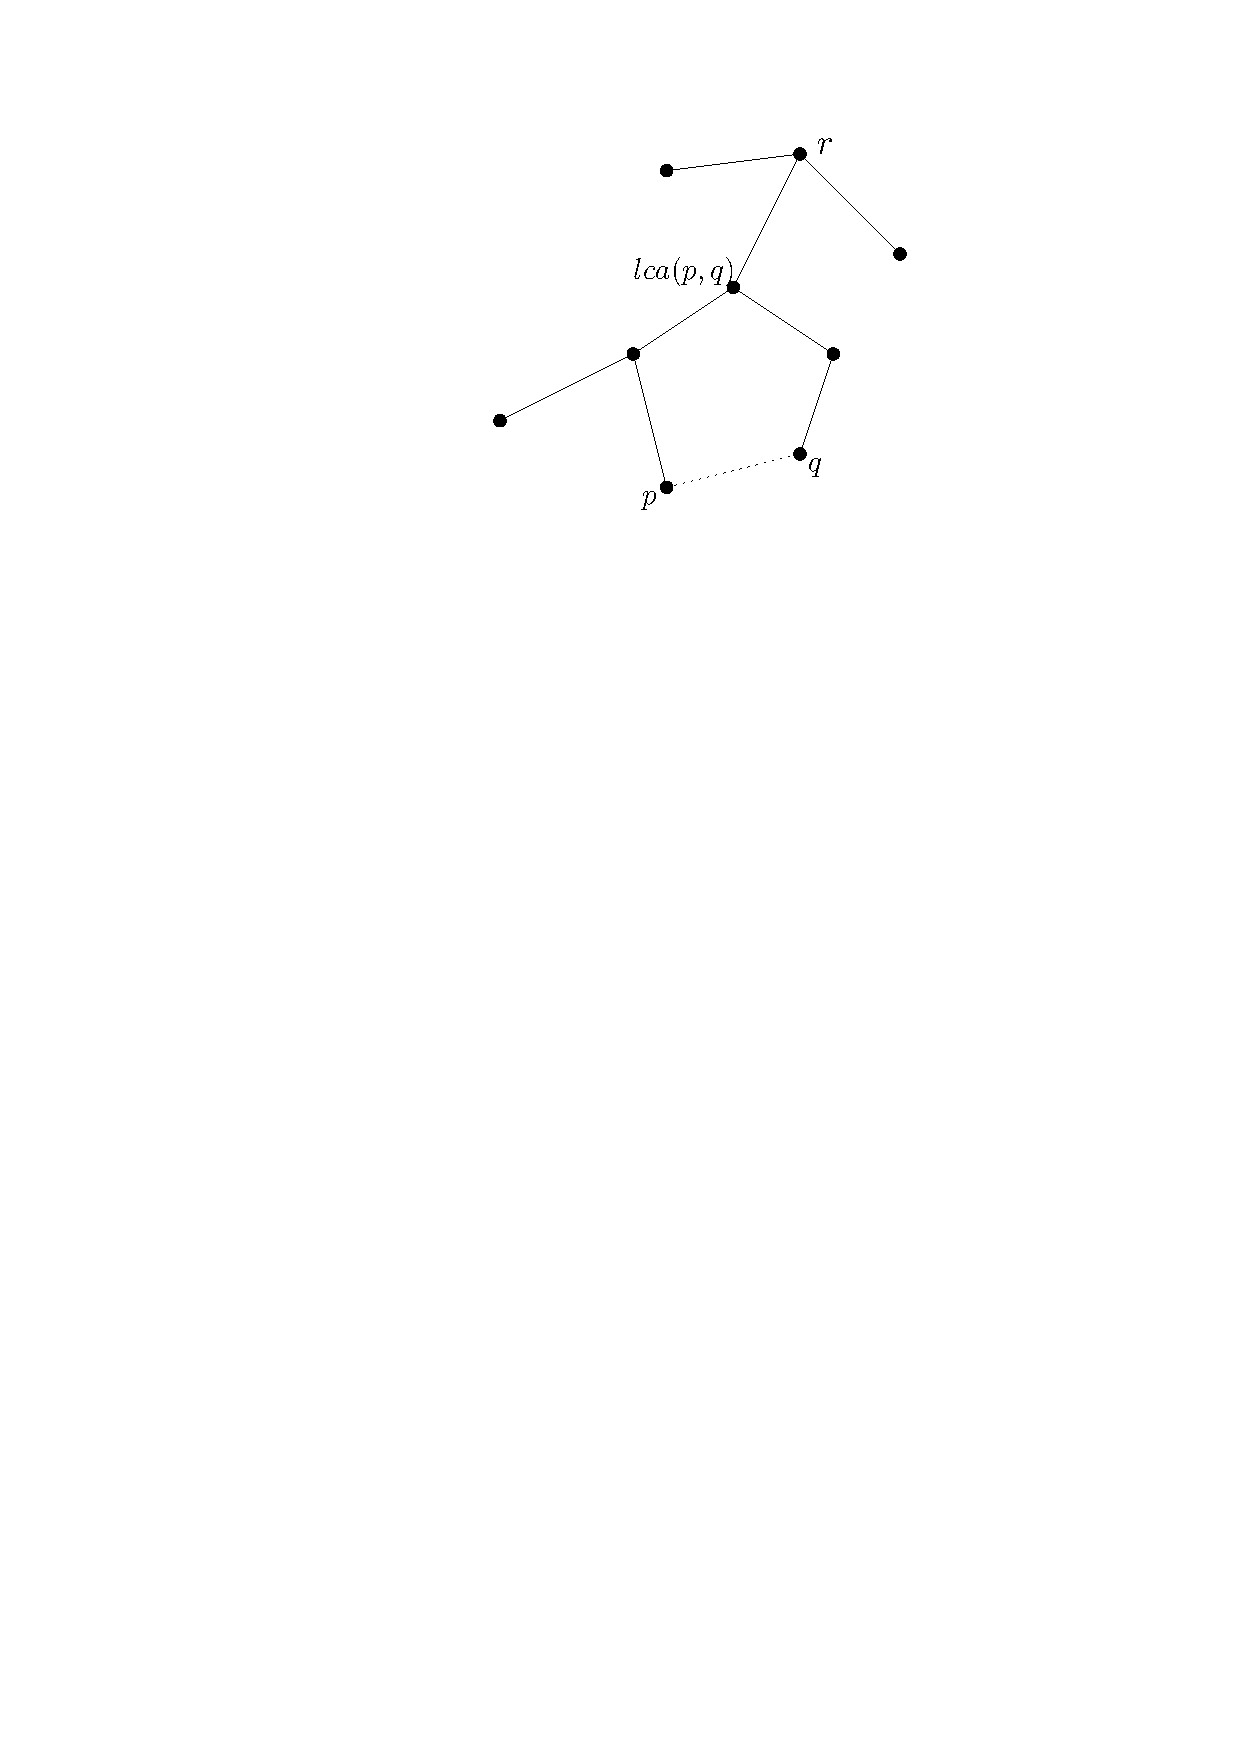
\includegraphics[scale=0.9]{pics/lca.pdf}}
\caption{Primer drevesa s korenom $r$ in ciklom, ki ga tvorita poti od $p$ do $r$ in $q$ do $r$, kjer pa obstaja tudi krajši cikel v poddrevesu s korenom $lca(p,q)$.}
\label{fig:lca}
\end{figure}

\bibliographystyle{abbrv}
\bibliography{biblia}
\end{document}
